\documentclass[11pt,a4paper]{report}
\newcommand{\volumetitle}{User Manual}
% Shared preamble of the two volumes of the manual: user_manual.tex (Volume 1, User Manual) and reference.tex
% (Volume 2, Reference and Verification). Each volume loads the class (report, 11pt, a4paper) and
% defines \volumetitle before reading this file.
\usepackage[T1]{fontenc}
\usepackage{mathpazo}
\usepackage[scaled=0.92]{helvet}
\usepackage[varqu,varl,scaled=0.96]{zi4}   % Inconsolata: a narrower, clearer monospace than Courier
\usepackage[protrusion=true,expansion=true]{microtype}
\DisableLigatures[-]{encoding=T1,family=tt*}   % "--" in \cmd{} stays two hyphens (not an en dash)
\usepackage[a4paper,margin=2.5cm,headheight=14pt]{geometry}
\usepackage{amsmath,amssymb}
\usepackage{booktabs,longtable,array,tabularx,multirow}
\usepackage{graphicx}
\usepackage[table]{xcolor}
\definecolor{brand}{HTML}{1F4E79}
\definecolor{brandlight}{HTML}{E3ECF6}
\definecolor{rowgray}{gray}{0.965}
\usepackage{tikz}
\usetikzlibrary{arrows.meta,positioning,shapes.geometric,calc,fit,backgrounds,decorations.pathmorphing,patterns}
\usepackage{algorithm}
\usepackage{algpseudocode}
\usepackage{listings}
\usepackage{caption}
\captionsetup{font=small,labelfont={bf,color=brand},skip=6pt}
\captionsetup[table]{position=top}
\usepackage[most]{tcolorbox}
\usepackage{needspace}
\usepackage{float}
\usepackage{etoolbox}
\usepackage{titlesec}
\titleformat{\chapter}[display]{\normalfont\color{brand}}{\sffamily\large\bfseries\MakeUppercase{\chaptertitlename}\ \thechapter}{4pt}{\raggedright\sffamily\huge\bfseries}[\vspace{3pt}{\titlerule[0.8pt]}]
\titlespacing*{\chapter}{0pt}{0pt}{18pt}
\titleformat{\section}{\needspace{8\baselineskip}\raggedright\normalfont\sffamily\Large\bfseries\color{brand}}{\thesection}{0.7em}{}
\titleformat{\subsection}{\needspace{6\baselineskip}\raggedright\normalfont\sffamily\large\bfseries\color{brand!80!black}}{\thesubsection}{0.7em}{}
\titleformat{\subsubsection}{\needspace{6\baselineskip}\normalfont\sffamily\normalsize\bfseries}{\thesubsubsection}{0.7em}{}
\titlespacing*{\section}{0pt}{16pt plus 4pt minus 2pt}{6pt}
\titlespacing*{\subsection}{0pt}{12pt plus 3pt minus 2pt}{4pt}
\usepackage{fancyhdr}
\pagestyle{fancy}
\fancyhf{}
\fancyhead[L]{\small\sffamily\color{gray}\leftmark}
\fancyhead[R]{\small\sffamily\color{gray}Raven--MODFLOW~6 coupling: \volumetitle}
\fancyfoot[C]{\small\sffamily\thepage}
\renewcommand{\headrulewidth}{0.4pt}
\renewcommand{\chaptermark}[1]{\markboth{\thechapter\quad #1}{}}
\fancypagestyle{plain}{\fancyhf{}\fancyfoot[C]{\small\sffamily\thepage}\renewcommand{\headrulewidth}{0pt}}
\usepackage{xr-hyper}   % references into the other volume (\externaldocument)
\usepackage[colorlinks=true,linkcolor=brand,citecolor=brand,urlcolor=brand]{hyperref}
\emergencystretch=6em
\setcounter{secnumdepth}{3}
\setcounter{tocdepth}{1}
\makeatletter\patchcmd{\l@chapter}{\addvspace{1.0em \@plus\p@}}{\addvspace{0.45em \@plus\p@}}{}{}\makeatother
\makeatletter\renewcommand*\l@section{\@dottedtocline{1}{1.5em}{2.9em}}\makeatother   % room for section numbers such as 10.11 and A.15
% ---- tables: small type, ragged-right columns, air between rows, shaded header row
\renewcommand{\arraystretch}{1.25}
\setlength{\tabcolsep}{5pt}
\AtBeginEnvironment{tabular}{\small}
\AtBeginEnvironment{tabularx}{\small}
\AtBeginEnvironment{longtable}{\small}
\newcolumntype{P}[1]{>{\raggedright\arraybackslash}p{#1}}
\newcolumntype{Y}{>{\raggedright\arraybackslash}X}
\newcommand{\hdr}{\rowcolor{brandlight}}
% ---- diagrams: the manual's sans-serif font; no hyphenation inside boxes
\tikzset{every picture/.prefix style={execute at begin picture={\sffamily}},
         every node/.append style={execute at begin node={\sffamily\hyphenpenalty=10000\exhyphenpenalty=10000}}}
% ---- code listings
\lstset{basicstyle=\ttfamily\footnotesize,columns=fullflexible,frame=single,framerule=0.3pt,rulecolor=\color{gray!50},breaklines=true,
        xleftmargin=4pt,xrightmargin=4pt,backgroundcolor=\color{gray!5},aboveskip=6pt,belowskip=6pt}
\newcommand{\ubreak}{\textunderscore}  % code names are not broken at underscores; a long one moves to the next line
\DeclareRobustCommand{\cmd}[1]{\begingroup\ttfamily\let\_\ubreak #1\endgroup}
\newcommand{\dt}{\Delta t}
% ---- boxes
\tcbset{boxrule=0.6pt,arc=2pt,left=5pt,right=5pt,top=3pt,bottom=3pt,fonttitle=\bfseries\small\sffamily}
\newtcolorbox{plain}{colback=teal!4,colframe=teal!55!black,title=In plain words}
\newtcolorbox{example}[1][]{colback=orange!4,colframe=orange!70!black,title=Worked example#1}
\newtcolorbox{watch}{colback=red!3,colframe=red!55!black,title=Watch out}
\newtcolorbox{inpractice}{colback=green!4,colframe=green!45!black,title=In practice}
\newtcolorbox{whattowrite}{colback=brandlight!40,colframe=brand,title=What to write}
\newtcolorbox{refcard}[1]{colback=brandlight!40,colframe=brand,title={Reference card: #1},breakable,enhanced jigsaw,before skip=10pt,after skip=10pt}

\externaldocument[R-]{reference}[Raven_MF6_Reference.pdf]   % Volume 2: \ref{R-label}
\begin{document}
\pagenumbering{Alph}
\begin{titlepage}
\centering
\vspace*{3.5cm}
{\color{brand}\rule{\linewidth}{1.2pt}}\par\vspace{16pt}
{\sffamily\bfseries\fontsize{30}{38}\selectfont\color{brand}Raven--MODFLOW~6\\[4pt]Groundwater Coupling\par}
\vspace{10pt}
{\sffamily\bfseries\LARGE\color{brand}Volume 1: User Manual\par}
\vspace{14pt}
{\color{brand}\rule{\linewidth}{1.2pt}}\par\vspace{24pt}
{\large Manual chapter for the Raven Hydrological Modelling Framework\\[2pt](based on Raven 4.15)\par}
\vfill
{\sffamily\Large\bfseries Rezgar Arabzadeh\par}
\vspace{4pt}
{\large Principal Scientist, Hazen and Sawyer\par}
\vspace{2cm}
{\large November 2026\par}
\vspace{1.2cm}
{\footnotesize\color{gray!70!black}\copyright\ 2026 Rezgar Arabzadeh. This manual is licensed under the Creative Commons Attribution 4.0
International License (CC BY 4.0), \url{https://creativecommons.org/licenses/by/4.0/}.\par}
\end{titlepage}
\pagenumbering{roman}
\begingroup\small\tableofcontents\endgroup
\cleardoublepage
\pagenumbering{arabic}
\chapter{What the coupling does}\label{uch:intro}\label{ch:c1}\label{ch:intro}
This chapter says what the coupling does and which pieces take part. It then says what is new for you, whether you
come from Raven or from MODFLOW.

\section{The problem this solves}
Raven \cite{craig2020raven} simulates the water cycle of a watershed: rain and snow, soil moisture, evaporation, runoff,
and flow in rivers and lakes. It divides a watershed into subbasins, and each subbasin into Hydrologic Response Units
(HRUs). An HRU is an area that behaves alike, for example forest on till, or a wetland.

Raven describes groundwater with simple ``buckets'' (linear reservoirs). Water enters a bucket and leaves it at a rate
proportional to what is stored. Buckets are fast and easy to calibrate. But they cannot say \emph{where} groundwater
flows, how deep the water table is at a well, how a pumping well lowers nearby streamflow, or whether a stream gains water
from the aquifer or loses water to it.

MODFLOW~6 \cite{langevin2017mf6} is the U.S. Geological Survey's groundwater model and the international standard for
those questions. It divides the underground into a three-dimensional grid of cells. It calculates the water level (the
\emph{head}) in every cell from the physics of flow through soil and rock. But MODFLOW has no snow, soil or evaporation
processes of its own: it must be told how much water reaches the water table.

The coupling joins the two so that each does what it is good at. Raven calculates everything at and near the land
surface. MODFLOW calculates the saturated groundwater below. The two exchange water every day.

\begin{plain}
Raven decides how much water soaks down to the water table. MODFLOW moves that water sideways and downwards through
the aquifer. Wherever the aquifer overflows --- into rivers, wetlands, lakes or back to the soil --- MODFLOW hands the
water back to Raven. Pumping wells and other stresses act on MODFLOW's side. Both models keep exact accounts, so not
a drop is created or lost at the boundary between them.
\end{plain}

\section{Two ways to use the coupling}\label{sec:twoways}
Most users are in one of two situations (Figure~\ref{fig:twoways}).
\begin{itemize}
\item \textbf{You already have a MODFLOW~6 model}, perhaps one calibrated over years. Raven connects to it and uses it as
      it is: same grid, same layers, same wells and boundaries (Chapter~\ref{uch:existing}).
\item \textbf{You have a Raven model but no groundwater model.} Raven builds one for you from your HRUs and a short
      description of the soil and rock layers under them (Chapter~\ref{uch:build}).
\end{itemize}
Everything else is the same in both cases: how water is exchanged, how the accounts are kept, the outputs and the tests.

\begin{figure}[!htbp]\centering% Which chapter to start from (TikZ; text is set by LaTeX, so boxes always fit their text)
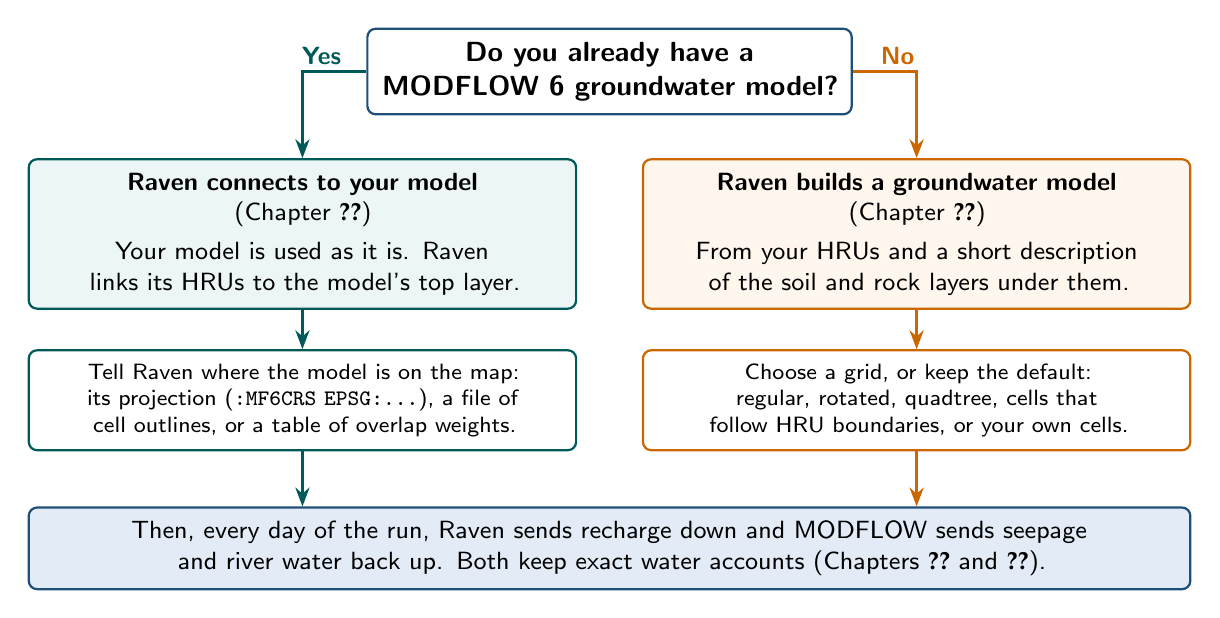
\begin{tikzpicture}[font=\sffamily\small,
  base/.style={rounded corners=3pt,line width=0.8pt,align=center,inner sep=5pt,execute at begin node={\hyphenpenalty=10000\exhyphenpenalty=10000}},
  q/.style={base,draw=brand,fill=white,text width=58mm,font=\sffamily\bfseries},
  yesA/.style={base,draw=teal!70!black,fill=teal!7,text width=66mm},
  noA/.style={base,draw=orange!80!black,fill=orange!7,text width=66mm},
  yesB/.style={base,draw=teal!70!black,fill=white,text width=66mm,font=\sffamily\footnotesize},
  noB/.style={base,draw=orange!80!black,fill=white,text width=66mm,font=\sffamily\footnotesize},
  fin/.style={base,draw=brand,fill=brandlight,text width=144mm},
  arr/.style={-{Stealth[length=2.4mm]},line width=0.9pt},
  lab/.style={font=\sffamily\bfseries\small,inner sep=2pt}]
\node[q] (q) at (0,0) {Do you already have a MODFLOW~6 groundwater model?};
\node[yesA,anchor=north] (y) at (-39mm,-11mm) {\textbf{Raven connects to your model}\\(Chapter~\ref{uch:existing})\\[3pt]Your model is used as it is. Raven links its HRUs to the model's top layer.};
\node[noA,anchor=north] (n) at (39mm,-11mm) {\textbf{Raven builds a groundwater model}\\(Chapter~\ref{uch:build})\\[3pt]From your HRUs and a short description of the soil and rock layers under them.};
\node[yesB,anchor=north] (y2) at ([yshift=-5mm]y.south) {Tell Raven where the model is on the map: its projection (\texttt{:MF6CRS EPSG:\dots}), a file of cell outlines, or a table of overlap weights.};
\node[noB,anchor=north] (n2) at ([yshift=-5mm]n.south) {Choose a grid, or keep the default: regular, rotated, quadtree, cells that follow HRU boundaries, or your own cells.};
\path let \p1=(y2.south), \p2=(n2.south) in coordinate (m) at (0,{min(\y1,\y2)-7mm});
\node[fin,anchor=north] (e) at (m) {Then, every day of the run, Raven sends recharge down and MODFLOW sends seepage and river water back up. Both keep exact water accounts (Chapters~\ref{uch:exchanges} and~\ref{uch:outputs}).};
\draw[arr,teal!70!black] (q.west) -| node[lab,pos=0.35,above,text=teal!70!black]{Yes} (y.north);
\draw[arr,orange!80!black] (q.east) -| node[lab,pos=0.35,above,text=orange!80!black]{No} (n.north);
\draw[arr,teal!70!black] (y.south) -- (y2.north);
\draw[arr,orange!80!black] (n.south) -- (n2.north);
\draw[arr,teal!70!black] (y2.south) -- (y2.south |- e.north);
\draw[arr,orange!80!black] (n2.south) -- (n2.south |- e.north);
\end{tikzpicture}

\caption{Which chapter to start from: connecting Raven to an existing MODFLOW~6 model, or letting Raven build one.}\label{fig:twoways}
\end{figure}

\section{How to use the two volumes}
The manual has two volumes. This one, the \emph{User Manual}, tells you what to write and what to expect. Volume~2,
\emph{Reference and Verification} (\cmd{Raven\_MF6\_Reference.pdf}), holds every rule and equation, the full tables of
commands and messages, the tests and the developer guide. In this volume, ``Reference, Section~4.3'' means Section~4.3
of Volume~2. Table~\ref{tab:readguide} says where to go.
\begin{table}[!htbp]\centering\small
\caption{Where to find what.}\label{tab:readguide}
\begin{tabularx}{\linewidth}{P{0.34\linewidth}Y}\toprule\hdr
If you want to\dots & Read\\\midrule
understand the idea & this chapter; groundwater in plain terms: Section~\ref{sec:newraven} and Reference, Chapter~\ref{R-ch:c2}\\
run a first coupled model & Chapter~\ref{uch:quick} (example \cmd{Liard\_groundwater})\\
let Raven build a groundwater model & Chapter~\ref{uch:build}; example \cmd{Liard\_groundwater}\\
connect Raven to your MODFLOW model & Chapter~\ref{uch:existing}; example \cmd{Liard\_existing\_model}\\
know what water moves where & Chapter~\ref{uch:exchanges}; the equations: Reference, Chapters~\ref{R-ch:c4} and~\ref{R-ch:c5}\\
read the results and check the water balance & Chapter~\ref{uch:outputs}\\
restart, run ensembles or calibrate & Chapter~\ref{uch:restarts}\\
fix a problem & Chapter~\ref{uch:trouble}; every message: Reference, Sections~\ref{R-app:errors} and~\ref{R-app:warnings}\\
look up a command or an output column & Chapter~\ref{uch:commands}; Reference, Chapter~\ref{R-ch:c6} and Appendix~\ref{R-app:tables}\\
see how the code was tested & Reference, Chapter~\ref{R-ch:c8}\\
change the code & Reference, Chapter~\ref{R-ch:c9}\\\bottomrule
\end{tabularx}
\end{table}
Technical words are explained in the glossary (Appendix~\ref{app:uglossary}). The workshops in
\cmd{docs/tutorials/workshops} of RavenHydroFramework-extra take you through the same steps with your own hands: Workshop~1
(getting started), 2 (your own groundwater model), 3 (the soil zone), 4 (an existing MODFLOW~6 model), 5 (restarts,
ensembles and particle tracking) and 6 (calibration with Ostrich).

\section{What you do, and what Raven does}
You work only with Raven's familiar text files:
\begin{enumerate}
\item mark which HRUs have groundwater underneath (\cmd{AQUIFER\_PROFILE} in the \cmd{.rvh} file);
\item describe the aquifer materials and their layering (\cmd{.rvp} file);
\item give the map of HRUs (a GeoJSON file) and, if you have them, land-surface and bedrock maps, rivers, wells,
monitoring wells and boundaries (the \cmd{.rvg} file, which the coupling adds to Raven's inputs);
\item switch the coupling on (\cmd{:GroundwaterModel MODFLOW6} in the \cmd{.rvi} file).
\end{enumerate}
Raven then does everything else by itself. It lays a grid over the HRUs and works out how much of each HRU lies in each
grid cell. It builds the layers from the land surface down to bedrock and writes a standard MODFLOW~6 model. It starts
MODFLOW, exchanges water every time step, and writes the results next to its usual outputs.

MODFLOW is used as a \emph{library}: a program part that another program can call. Raven talks to it through MODFLOW's
official programming interface \cite{hughes2022xmi}. No MODFLOW source code is changed.

\section{What is new for a Raven user}\label{sec:newraven}
If you know Raven but not MODFLOW, these are the new ideas. Reference, Chapter~\ref{R-ch:c2}, explains them with
equations and numbers.
\begin{itemize}
\item \textbf{Head.} The level to which water rises in a well, in metres above sea level. Groundwater flows from high
head to low head. Near the surface the head is the water table.
\item \textbf{Cells and layers.} MODFLOW computes one head per cell. The cells form layers, from the model top down to
bedrock. A column is the stack of cells at one map location.
\item \textbf{Hydraulic conductivity} ($K$, m/d) says how easily water moves through a material: gravel passes water
fast, clay very slowly. Flow between two cells is the head difference times a conductance, which comes from $K$, the
cell sizes and the thickness of saturated material.
\item \textbf{Storage.} When the water table falls, the pores drain; the specific yield ($S_y$) is the share of the volume
that drains. A full (confined) layer releases far less water, through the specific storage ($S_s$).
\item \textbf{Boundaries.} Rivers, drains, wells and fixed heads add or remove water at chosen cells. Many of them depend
on the head: a river leaks into the aquifer when the head is below the river, and gains water when it is above.
\item \textbf{Your \cmd{GROUNDWATER} store changes role.} In a coupled HRU it is a pass-through: whatever enters it during
a day is handed to MODFLOW as recharge that day. Baseflow then comes from the aquifer, not from a bucket.
\end{itemize}

\section{What is new for a MODFLOW user}\label{sec:newmodflow}
If you know MODFLOW but not Raven, these are the new ideas.
\begin{itemize}
\item \textbf{HRUs and subbasins.} Raven's land units are HRUs, grouped into subbasins; each subbasin drains to one river
reach. Raven computes each HRU's water budget, then routes the runoff down the river network.
\item \textbf{State variables.} Raven keeps water in named stores per HRU: \cmd{SOIL[0]}, \cmd{SOIL[1]}, \dots,
\cmd{DEPRESSION}, \cmd{SURFACE\_WATER}, \cmd{GROUNDWATER} and others. Processes in the \cmd{.rvi} file move water between
them; for example \cmd{:Percolation PERC\_CONSTANT FAST\_RESERVOIR GROUNDWATER} moves water from one store to
another.
\item \textbf{Recharge is computed, not given.} Raven's snow, soil and evaporation processes decide how much water
reaches the water table each day. Your RCH and EVT packages are replaced by Raven's (Chapter~\ref{uch:existing}).
\item \textbf{The files.} \cmd{.rvi} holds the options and processes, \cmd{.rvh} the subbasins and HRUs, \cmd{.rvp} the
parameters, \cmd{.rvt} the time series (forcing, well rates, observations), \cmd{.rvc} the initial conditions. The
coupling adds the \cmd{.rvg} file (Table~\ref{tab:ufiles}).
\item \textbf{Time.} Raven steps through time, usually one day at a time. MODFLOW runs one Raven step per MODFLOW time
step; your stress periods are kept and split into Raven steps.
\item \textbf{Calibration.} Raven is often calibrated with Ostrich against streamflow; with the coupling, heads at
monitoring wells join the objective.
\end{itemize}

\section{The pieces}\label{ch:overview}
\subsection{Who owns which water}
Every drop of water in the coupled system belongs to exactly one of the two models at any time:
\begin{itemize}
\item \textbf{Raven} owns snow, canopy, soil and vadose-zone stores, depressions and wetlands, rivers, lakes and
reservoirs.
\item \textbf{MODFLOW} owns the saturated groundwater below the \emph{model top}.
\end{itemize}
By default the model top is the land surface. Users with physically based soil layers can lower it with
\cmd{SOIL\_ZONE\_DEPTH}. Or, with \cmd{:SoilZone PHYSICAL}, they can hand the soil layers to Raven and let the water table
rise into them, as in GSFLOW \cite{markstrom2008gsflow} (Section~\ref{sec:usoilzone}).

On sloping and irregular land each cell then samples the DEM at many points. So the soil saturates first at the foot of
a slope and in hollows, and the saturated area spreads up and retreats down the slope with the water table
(Section~\ref{sec:applysz}; the rules: Reference, Section~\ref{R-sec:szslope}). Below the soil, recharge can cross an
unsaturated zone (Richards' equation, a kinematic wave or a storage cascade), and dry soil draws water up from a shallow
water table by capillary rise (Reference, Sections~\ref{R-sec:szvadose} and~\ref{R-sec:szcaprise}).

Water moves between the two models only through the exchanges of Chapter~\ref{uch:exchanges}, and each exchange is
recorded on both sides. In a coupled HRU, Raven's \cmd{GROUNDWATER} store is a \emph{pass-through}: whatever enters it
during a day is handed to MODFLOW as recharge that day.

\subsection{The software}
Figure~\ref{fig:arch} shows the parts. The \emph{model builder} runs once at the start: it reads the inputs and writes a
standard MODFLOW~6 model. The \emph{exchange} runs every time step.
\begin{figure}[!htbp]\centering
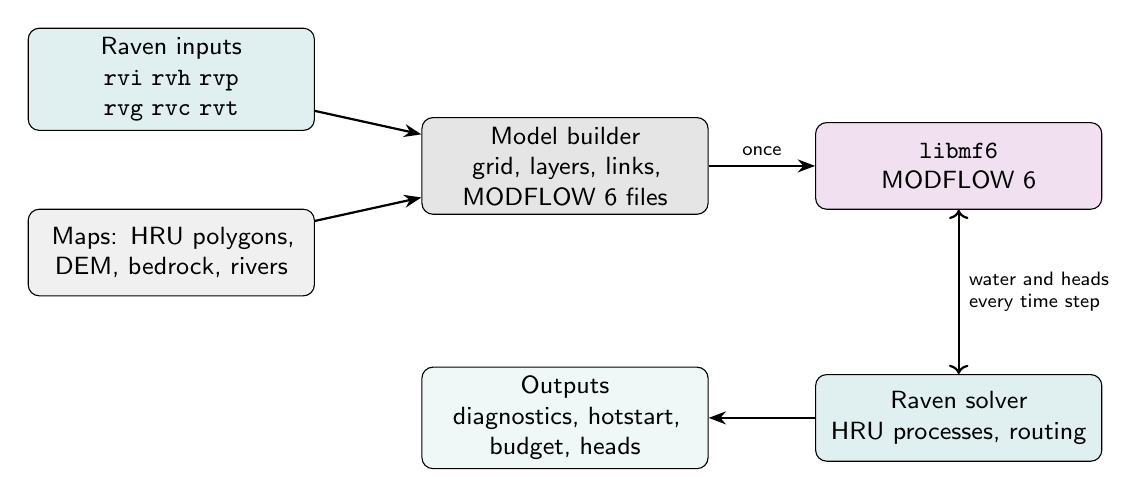
\begin{tikzpicture}[box/.style={draw,rounded corners,align=center,minimum height=11mm,text width=34mm,font=\small},
 ar/.style={-{Stealth[length=2.2mm]},thick}]
\node[box,fill=teal!12] (in) at (0,1.1) {Raven inputs\\ \cmd{rvi rvh rvp rvg rvc rvt}};
\node[box,fill=gray!12] (geo) at (0,-1.1) {Maps: HRU polygons, DEM, bedrock, rivers};
\node[box,fill=gray!20] (bld) at (5,0) {Model builder\\ grid, layers, links,\\ MODFLOW 6 files};
\node[box,fill=violet!12] (mf) at (10,0) {\cmd{libmf6}\\ MODFLOW 6};
\node[box,fill=teal!12] (rv) at (10,-3.2) {Raven solver\\ HRU processes, routing};
\node[box,fill=teal!6] (out) at (5,-3.2) {Outputs\\ diagnostics, hotstart,\\ budget, heads};
\draw[ar] (in) -- (bld); \draw[ar] (geo) -- (bld);
\draw[ar] (bld) -- node[above,font=\scriptsize]{once} (mf);
\draw[ar,<->] (mf) -- node[right,font=\scriptsize,align=left]{water and heads\\ every time step} (rv);
\draw[ar] (rv) -- (out);
\end{tikzpicture}
\caption{The software pieces. The builder runs once per simulation (or per ensemble member); the exchange runs every
time step.}\label{fig:arch}
\end{figure}

\subsection{One day of the coupled model}
This happens every time step (one day in the examples). Reference, Section~\ref{R-ch:timestep}, gives the exact
algorithm.
\begin{enumerate}
\item \textbf{Raven's land-surface day.} Raven calculates snowmelt, infiltration, evaporation and flow between its soil
layers. In coupled HRUs, water that percolates past the soil ends up in \cmd{GROUNDWATER}.
\item \textbf{Recharge handed over.} The water in each HRU's \cmd{GROUNDWATER} is spread over the grid cells under that
HRU, in proportion to how much of the HRU lies in each cell.
\item \textbf{Stresses set.} River levels (from Raven's rivers at the start of the day), well pumping rates, boundary
heads, wetland and lake levels, and the evaporation demand not met by Raven are passed to MODFLOW.
\item \textbf{MODFLOW's day.} MODFLOW calculates new heads everywhere, with the flows to and from rivers, drains,
wells and boundaries.
\item \textbf{Water handed back.} Groundwater that seeps out at the land surface is added to a Raven store of the HRUs
above. Groundwater that discharges to rivers is added to the river inflow of the subbasin. River losses are taken from
the river. Wetland and lake exchanges change those Raven stores.
\item \textbf{Raven's river day.} Raven routes water down the river network, with the groundwater contributions.
Reservoirs compute their seepage using the aquifer head beneath them.
\item \textbf{Accounts.} Both models update their water balances, and the groundwater outputs are written.
\end{enumerate}

\section{Main features}
\begin{itemize}
\item Any number of \emph{aquifer profiles} (layer stacks), each with any number of layers. Layer types: aquifer,
confined aquifer, aquitard (confining layer) and aquiclude.
\item Land surface and bedrock from raster maps. Layers that thin out against bedrock are handled automatically.
\item Coupling to an existing MODFLOW~6 model. Raven links its HRUs to the model's top active layer and leaves the model
intact, with built-in map projections, unit conversion and safeguards against double counting
(Chapter~\ref{uch:existing}).
\item Five grid options: the default regular grid, rotated and refined regular grids, quadtree grids, meshes whose cells
follow HRU boundaries, and imported cells. Layers can be connected by elevation (Section~\ref{sec:ugrids}).
\item Water exchanges: recharge (with optional delay), groundwater seepage at the land surface, rivers (gaining and
losing), evaporation from a shallow water table, wetlands and lakes held in Raven stores, Raven reservoirs, pumping and
injection wells, head-dependent and fixed-head boundaries.
\item Cells can dry out and rewet; areas of aquifer can disconnect and reconnect by themselves.
\item Monitoring wells: simulated heads are written out and scored against observations like streamflow, so the
groundwater parameters can be calibrated (for example with Ostrich).
\item Hotstart (continuing a run from where another ended), ensembles, NetCDF output of the whole head field.
\item Exact water accounting on both sides, checked automatically by an audit tool supplied with the code.
\end{itemize}

\section{Design principles}
\begin{enumerate}
\item \textbf{Raven is the single user interface.} All inputs are Raven files; MODFLOW files are generated.
\item \textbf{Standard MODFLOW only.} Only standard MODFLOW~6 packages are used; the generated model can be opened in
FloPy or ModelMuse.
\item \textbf{Each fact is entered once.} Geometry comes from maps, hydrogeology from profiles, time-varying stresses
from time series.
\item \textbf{Generic.} Nothing is specific to a basin; any Raven model can couple any subset of its HRUs.
\item \textbf{Exact accounting.} Every exchanged volume is computed once and applied identically on both sides.
\item \textbf{No surprise for existing users.} Models without groundwater give bit-for-bit the same results as
Raven~4.15 (the version this coupling is built on), except in the few cases where the coupled code corrects Raven
itself: models with reservoirs, ensembles and age-tracer runs started from a hotstart file (Reference,
Table~\ref{R-tab:ravendiff}). Raven still builds and runs without MODFLOW installed.
\end{enumerate}

\section{Scope and assumptions}
\begin{itemize}
\item \textbf{What MODFLOW simulates:} saturated groundwater flow (Darcy flow, storage change) in a layered aquifer
system under the coupled HRUs, with dry and rewetting cells.
\item \textbf{What stays in Raven:} everything above the model top --- snow, canopy, soil and unsaturated zone, surface
runoff, depressions, rivers, lakes and reservoirs --- and all HRUs without an aquifer profile.
\item \textbf{Water density and temperature} are constant. There is no salt-water or heat transport.
\item \textbf{No constituent transport.} The coupling exchanges water, not constituent mass. So Raven's \cmd{:Transport}
(tracers, nutrients, the age tracer, temperature) is not available in a coupled run; the run stops with a message.
\item \textbf{The grid} is regular (square cells, optionally rotated), a quadtree, an HRU mesh whose cells follow HRU
boundaries, or imported cell polygons (Section~\ref{sec:ugrids}). An existing MODFLOW~6 model keeps its own DIS or DISV
grid (Chapter~\ref{uch:existing}). A generated model covers the cells that the coupled HRUs cover.
\item \textbf{Time:} both models use Raven's time step (daily or shorter). Exchanges are explicit between the models at
the step level, but every head-dependent exchange is implicit inside MODFLOW. With \cmd{:SoilZone PHYSICAL} the
soil--aquifer interface is also iterated inside MODFLOW's outer iterations (Reference, Section~\ref{R-sec:szinterface}).
\end{itemize}

\section{When to use the coupling, and when not to}
Use it when the question involves the \emph{spatial} behaviour of groundwater: the water-table depth at a location, the
effects of pumping on streams, gaining and losing reaches, groundwater flow between subbasins, wetlands fed by
groundwater, the drought recession of large aquifers, or when head measurements should constrain the model.

Raven's conceptual baseflow remains the better choice for fast screening, very large ensembles, or basins without a
significant aquifer.

\section{What changes for an existing Raven model}
\begin{itemize}
\item Nothing, unless \cmd{:GroundwaterModel MODFLOW6} is added. Results then stay bit-for-bit identical to Raven~4.15,
except where the coupled code corrects Raven itself (Reference, Table~\ref{R-tab:ravendiff}):
  \begin{itemize}
  \item models with reservoirs: absolute-stage reservoirs without an initial stage start at their crest, a drying
  reservoir books only the water it has, and \cmd{solution.rvc} carries stages and flows with 12 digits;
  \item ensembles: every member starts from the first run's state;
  \item age-tracer runs started from a hotstart file: the ages continue from the run that wrote the file.
  \end{itemize}
\item With the coupling on, coupled HRUs lose their conceptual deep-groundwater behaviour: their \cmd{GROUNDWATER} store
becomes a pass-through, and their baseflow comes from the aquifer via seepage and river exchange.
\item Run times increase. The 20-year Liard run (3\,252 active columns) takes about 10 minutes instead of 35 seconds on
one processor core.
\end{itemize}

\section{Files at a glance}
\begin{table}[!htbp]\centering
\caption{Input and output files of the coupling.}\label{tab:ufiles}
\begin{tabular}{P{0.2\linewidth}P{0.748\linewidth}}\toprule\hdr
File & Role in the coupling\\\midrule
\cmd{.rvi} & switch on (\cmd{:GroundwaterModel MODFLOW6}); route recharge into \cmd{GROUNDWATER}\\
\cmd{.rvh} & \cmd{AQUIFER\_PROFILE} per HRU; reservoirs with \cmd{:SeepageParameters}\\
\cmd{.rvp} & aquifer classes, profiles and profile parameters\\
\cmd{.rvg} & geometry (HRU polygons, maps, rivers), grid, wells, monitoring wells, boundaries, options\\
\cmd{.rvt} & well rates, boundary heads, observed heads\\
\cmd{.rvc} & initial heads; hotstart blocks written by Raven\\
GeoJSON, ASCII grids & HRU polygons, river lines, boundary shapes; DEM and bedrock maps\\
\cmd{<output>/mf6/} & generated MODFLOW 6 model and its own outputs\\\bottomrule
\end{tabular}
\end{table}

\chapter{Quick start with example A}\label{uch:quick}\label{ch:c7}
This chapter runs the first coupled model: example~A, \cmd{examples/Liard\_groundwater}, in which Raven builds the
groundwater model. It shows every line added to an ordinary Raven model. The same steps, with more explanation, are
Workshop~1.

\begin{plain}
This chapter walks through a real example --- the Liard River in northern Canada --- from input files to results.
Chapter~\ref{uch:build} then shows how to set up your own watershed.
\end{plain}

\section{Install Raven and the MODFLOW~6 library}\label{sec:uinstall}
\begin{enumerate}
\item Get Raven with the coupling (RavenHydroFramework). The coupling is offered to the Raven team for inclusion; until it
is part of Raven, use the \cmd{mf6-coupling} branch of \url{https://github.com/rarabzad/RavenHydroFramework}. Beside it,
get RavenHydroFramework-extra (branch \cmd{main} of \url{https://github.com/rarabzad/RavenHydroFramework-extra};
Reference, Section~\ref{R-sec:building}).
\item Build Raven with CMake: \cmd{cmake -S . -B build}, then \cmd{cmake --build build --config Release} (an optimised
\cmd{Release} build by default).
\item The same build gets the MODFLOW~6 library. With a Fortran compiler, meson~$\geq$~1.7, ninja and git, and the
MODFLOW~6 repository reachable, it builds the library from source. Otherwise (also offline) it downloads the official
release library (Linux x86\_64, Windows x64, Apple Silicon Macs). Either way the library ends up next to Raven, which
finds it without any setting (Reference, Section~\ref{R-sec:building}).
\item If Raven was built without the library (\cmd{make} in \cmd{src/}, \cmd{src/Raven.sln}, \cmd{-DRAVEN\_MF6=OFF}, or
the configure warned that it found no way to get it), get it with \cmd{python tools/get\_mf6.py} in the
RavenHydroFramework-extra repository (Reference, Section~\ref{R-sec:getmf6}). The coupling needs MODFLOW~6.5 or newer; it
was tested with 6.8.1 and 6.6.3, and 6.8 or newer is recommended.
\item \cmd{get\_mf6.py} has no library for Linux other than x86\_64 (e.g.\ aarch64), for Windows on ARM64, or for Intel
Macs (only with \cmd{--version 6.6.3}). There, build the library with Raven: \cmd{cmake -S . -B build -DRAVEN\_MF6=SOURCE},
or give a library you have with \cmd{-DRAVEN\_MF6=PATH -DRAVEN\_MF6\_PATH=/path/to/libmf6.so}.
\end{enumerate}
\begin{inpractice}
\cmd{examples/README.md} gives these steps command by command for Windows, Linux and macOS. The release package for
Linux has Raven and the library ready in its \cmd{bin/} folder.
\end{inpractice}

\section{The example}\label{ch:tutorial}
Example~A is the Liard River model (65 subbasins, 1\,107 HRUs, northern British Columbia and Yukon) with an aquifer
added under three nested subbasins (52, 48 and 43; about 13\,800 km$^2$, 85 coupled HRUs). The other 62 subbasins run
exactly as they do without groundwater.

The original Liard package was made for Raven 2.9.1. For Raven 4.x its Windows paths use \texttt{/}, and the parameter
\cmd{DEP\_THRESHHOLD} is spelled \cmd{DEP\_THRESHOLD}. The example files already include these changes.

Four of Raven's files change. The next four sections show what was added to each.

\section{Step 1: mark the HRUs with groundwater (.rvh)}
In the \cmd{:HRUs} table, the \cmd{AQUIFER\_PROFILE} column was filled for the HRUs of subbasins 52, 48 and 43:
\cmd{VALLEY\_ALLUVIUM} for forest, shrub and wetland HRUs; \cmd{UPLAND\_TILL} for barren HRUs. Glaciers keep
\cmd{[NONE]}. A group listing the same HRUs was added at the end of the file:
\par\noindent\begin{minipage}{\linewidth}
\begin{lstlisting}
:HRUGroup AquiferHRUs
  2736, 2745, 2747, ...
:EndHRUGroup
\end{lstlisting}
\end{minipage}\par\smallskip

\section{Step 2: describe the aquifer (.rvp)}
Added at the end of \cmd{Liard.rvp}:
\begin{lstlisting}
:AquiferClasses
  :Attributes, K_HORIZ, K_VERT, SPEC_STORAGE, SPEC_YIELD, POROSITY
  :Units,      m/d,     m/d,    1/m,          none,       none
  GRAVEL,      50.0,    5.0,    1.0E-5,       0.25,       0.30
  CLAY_TILL,   0.001,   0.0001, 1.0E-4,       0.03,       0.40
  SAND,        10.0,    1.0,    1.0E-5,       0.20,       0.35
  UPLAND_TILL, 0.2,     0.02,   1.0E-4,       0.08,       0.30
:EndAquiferClasses

:AquiferProfiles
  VALLEY_ALLUVIUM, 3, GRAVEL, 15.0, AQUIFER, CLAY_TILL, 5.0, AQUITARD, SAND, TO_BEDROCK, CONFINED_AQUIFER
  UPLAND_TILL,     1, UPLAND_TILL, TO_BEDROCK, AQUIFER
:EndAquiferProfiles

:AquiferProfileParameters
  :Attributes,     INITIAL_HEAD_DEPTH, DEFAULT_BEDROCK_DEPTH, SEEPAGE_LEAKANCE, SOIL_ZONE_DEPTH
  :Units,          m,                  m,                     1/d,              m
  VALLEY_ALLUVIUM, 3.0,                60.0,                  1.0,              0.0
  UPLAND_TILL,     8.0,                15.0,                  1.0,              0.0
:EndAquiferProfileParameters
\end{lstlisting}
The valley aquifer is a gravel layer (15 m) over a clay-till aquitard (5 m) over sand down to bedrock. The uplands have
one till layer down to shallow bedrock. Section~\ref{sec:uprofiles} explains each block.

\section{Step 3: switch the coupling on and send recharge to it (.rvi)}
\par\noindent\begin{minipage}{\linewidth}
\begin{lstlisting}
:GroundwaterModel MODFLOW6
:DefineHRUGroups AquiferHRUs
...
:Percolation PERC_CONSTANT FAST_RESERVOIR SLOW_RESERVOIR
  :-->Conditional HRU_GROUP IS_NOT AquiferHRUs     # existing process, only for uncoupled HRUs
:Percolation PERC_CONSTANT FAST_RESERVOIR GROUNDWATER
  :-->Conditional HRU_GROUP IS AquiferHRUs         # new: this water becomes recharge
\end{lstlisting}
\end{minipage}\par\smallskip
Seepage returns to the lowest soil layer (\cmd{SLOW\_RESERVOIR}), whose existing baseflow process carries it to the
rivers. Aquifer--river exchange goes directly to the reaches.

\section{Step 4: the groundwater file (.rvg)}
\begin{lstlisting}
#########################################################################
# Liard.rvg - Raven-MODFLOW 6 groundwater file (Liard River test case)
#   Groundwater under Central Liard subbasins 52 -> 48 -> 43 (85 HRUs).
#   Hydrogeology (aquifer classes, profiles) is in Liard.rvp;
#   which HRUs have groundwater is set by AQUIFER_PROFILE in Liard.rvh.
#########################################################################

# --- geometry (stand-in data built by tools_build_standin_inputs.py; replace with real data) ---
:HRUGeometry        Liard_HRUs_standin.geojson  HRU_ID    # HRU polygons, lon/lat
:RiverGeometry      Liard_rivers.geojson                  # river lines (subbasin assigned automatically)
:LandSurface        Liard_dem_standin.asc                 # DEM, ESRI ASCII, lon/lat
:BedrockSurface     Liard_bedrock_standin.asc             # bedrock elevation, same format

# --- grid and coupling settings ---
:GridCellSize       2000.0     # m
:MinCellCoverage    0.25       # fraction of a cell covered by coupled HRUs to activate it
:HeadSaveFrequency  365        # steps between saves of the full head field (mf6/gwf.hds)
# :MF6Library       /path/to/libmf6.so    # only if Raven does not find it by itself (or RAVEN_MF6_LIB)

# --- optional features (uncomment to use; see the user guide) ---
# :GWInitialization  STEADY_STATE 0.45            # steady-state start, uniform recharge [mm/d]
# :SurfaceWaterExchange DEPRESSION WetlandHRUs LEAKANCE 0.01   # wetlands <-> aquifer
# :WriteNetCDFHeads                               # GWHeads.nc (Raven built with -Dnetcdf)
# :ReservoirExchange                              # Raven reservoirs (with :SeepageParameters) <-> aquifer
# :Wells
#   :Attributes, NAME, LATITUDE, LONGITUDE, SCREEN_TOP, SCREEN_BOT
#   1, PW_1, 59.27310, -124.73460, 1199.7, 1188.7
# :EndWells                                        # rates: :WellFlowRate 1 m3/d ... in Liard.rvt
# :ObservationWells
#   :Attributes, NAME, LATITUDE, LONGITUDE, SCREEN_ELEV
#   101, OW_NEAR, 59.27310, -124.73060, 1192.7
# :EndObservationWells                             # data: :ObservationData GW_HEAD 101 m ... in Liard.rvt
# head boundaries: a HEAD (or a :BoundaryHead series in Liard.rvt) must lie above the bottoms of the cells it is to hold;
# the top layer under these two lies between about 1300 and 1315 m (3 GHB and 9 CHD cells with these heads)
# :GeneralHeadBoundary   GHB1 boundary_line.geojson HEAD 1310.0 CONDUCTANCE 5000.0 LAYERS TOP
# :SpecifiedHeadBoundary LAKE1 lake.geojson HEAD 1312.0 LAYERS TOP
\end{lstlisting}
The HRU polygons, DEM and bedrock of this example are \emph{stand-ins}. The Liard package has no HRU polygons, DEM or
bedrock map, so \cmd{tools\_build\_standin\_inputs.py} made them: Voronoi polygons around the HRU centroids clipped to
each subbasin, a DEM interpolated from HRU elevations, and bedrock 60 m (valley), 15 m (upland) and 5 m (glacier) below
it. For a real study, replace them with real data.

\section{Step 5: run}
\par\noindent\begin{minipage}{\linewidth}
\begin{lstlisting}
cd examples/Liard_groundwater
../../Raven.exe Liard -o output/
python3 tools_audit.py output        # optional automated check
\end{lstlisting}
\end{minipage}\par\smallskip
(Use the path of your own Raven program in place of \cmd{../../Raven.exe}.) The 20-year daily run takes about 10 minutes
on one processor core (35 seconds without groundwater). For a quick first try, set \cmd{:Duration} in \cmd{Liard.rvi} to
365 days instead of 7305. Raven prints the date as it goes, and the last line is \cmd{Exiting Gracefully: Successful
Simulation}.

Raven builds a grid of 3 layers $\times$ 85 $\times$ 54 cells of 2 km, with 3\,252 active columns and 178 river cells
(Figure~\ref{fig:ugrid}).
\begin{figure}[!htbp]\centering
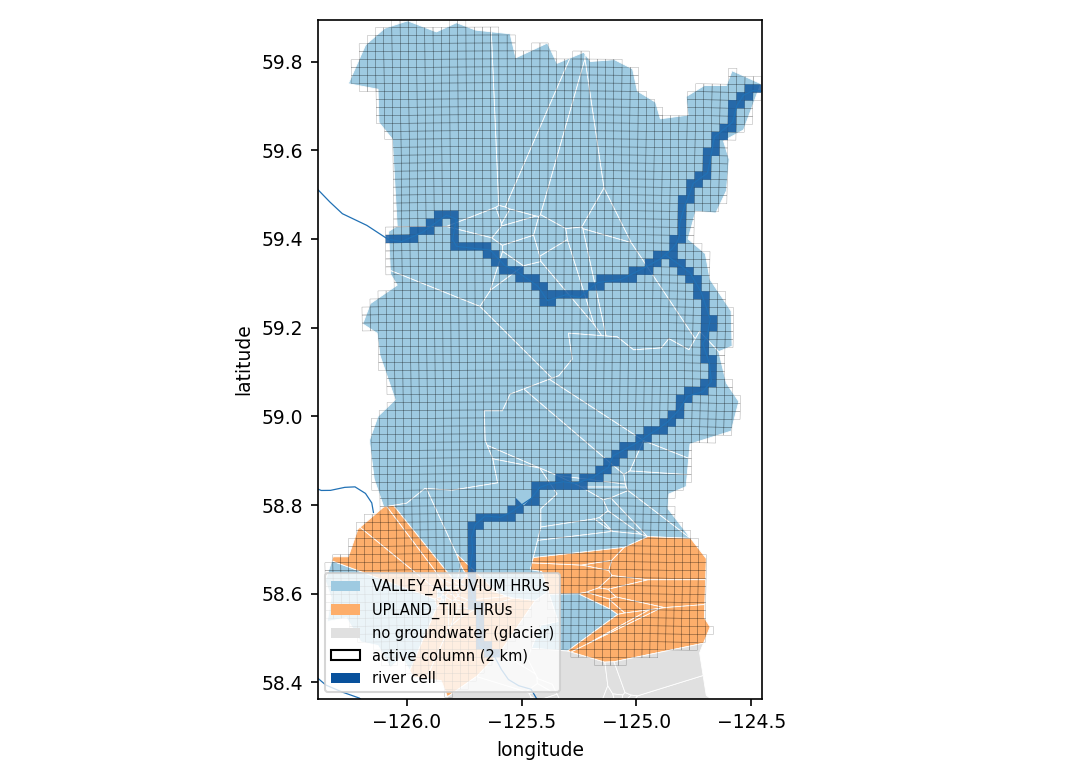
\includegraphics[width=0.9\linewidth]{figures/fig_grid_liard.png}
\caption{Example~A: coupled HRUs (colour = aquifer profile), active 2~km columns and river cells.}\label{fig:ugrid}
\end{figure}

\section{Step 6: look at the results}
\begin{itemize}
\item \cmd{GWModelSummary.txt}: check the grid, the number of active cells, and that every coupled HRU is linked.
\item \cmd{GWBudget.csv}: the daily groundwater balance (Figure~\ref{fig:budget}). The error column should stay tiny.
\item \cmd{GWHRUState.csv}: the depth to water under each HRU. Figure~\ref{fig:wtdepth} shows the map from
\cmd{mf6/gwf.hds}.
\item \cmd{Hydrographs.csv}: streamflow includes groundwater discharge (Figure~\ref{fig:hydro}).
\end{itemize}
\begin{figure}[!htbp]\centering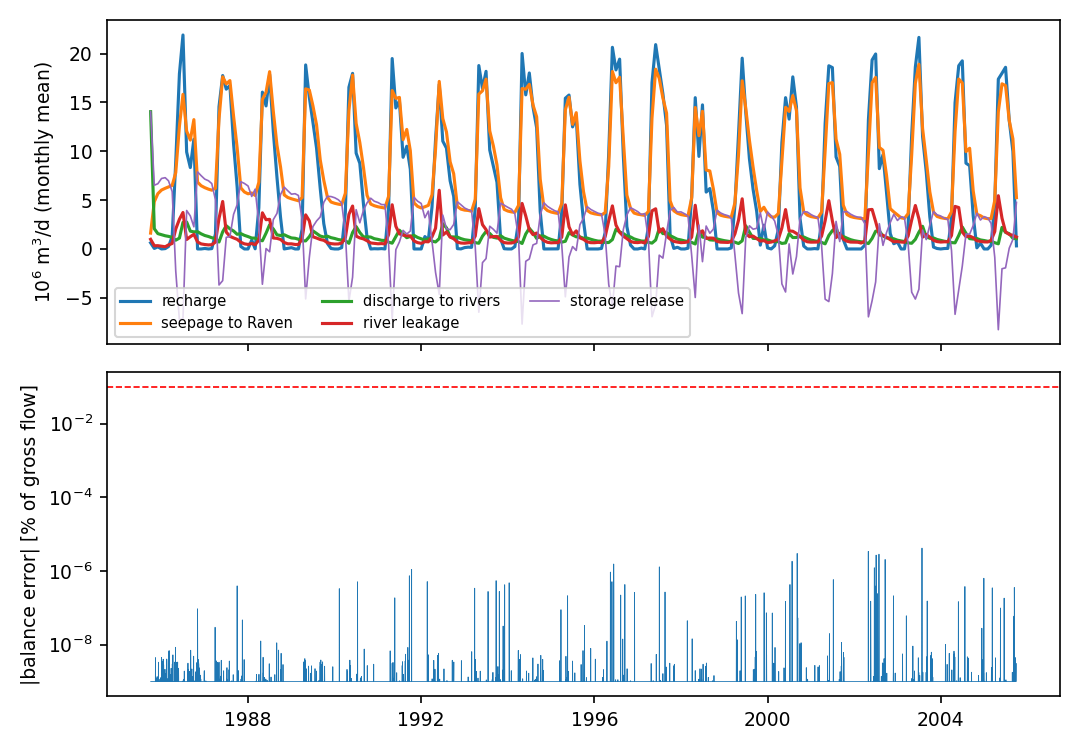
\includegraphics[width=\linewidth]{figures/fig_budget.png}
\caption{Groundwater budget of the 20-year Liard run (monthly means) and daily balance error; the dashed line is 0.1\%.}\label{fig:budget}\end{figure}
\begin{figure}[!htbp]\centering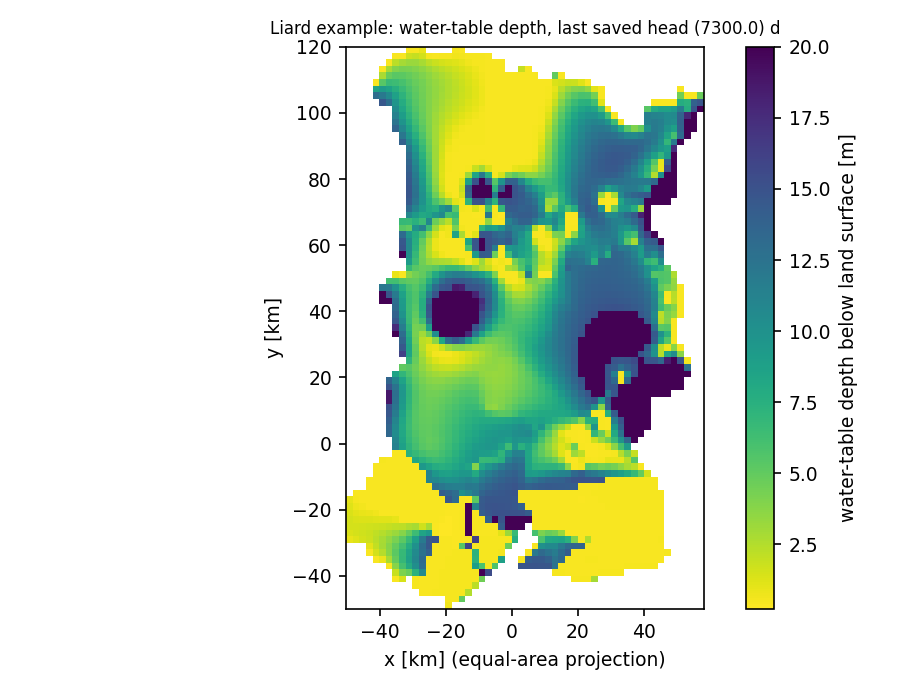
\includegraphics[width=0.72\linewidth]{figures/fig_wtdepth.png}
\caption{Depth to water at the last saved head.}\label{fig:wtdepth}\end{figure}
\begin{figure}[!htbp]\centering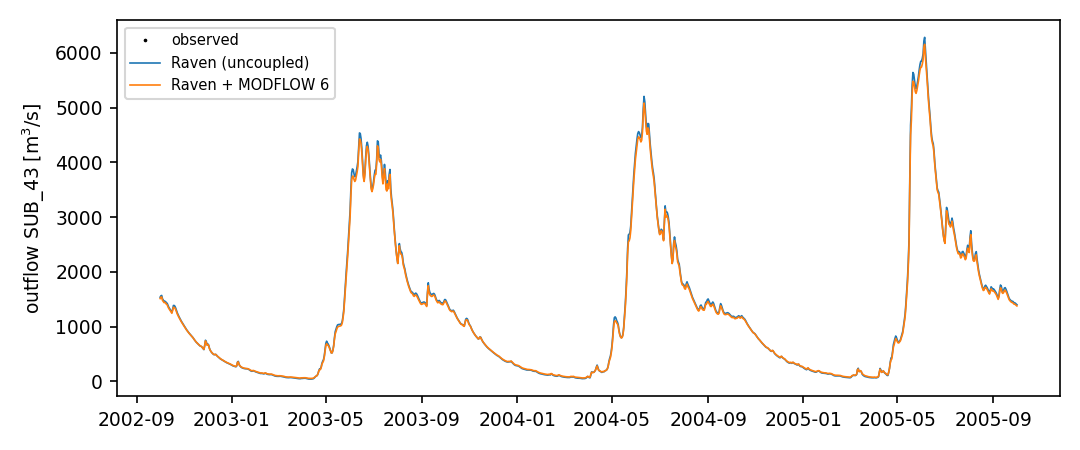
\includegraphics[width=\linewidth]{figures/fig_hydrograph.png}
\caption{Outflow of subbasin 43, 2003--2005, without and with groundwater (not recalibrated).}\label{fig:hydro}\end{figure}
Without recalibration and with stand-in geometry, the Nash--Sutcliffe efficiency at gauges 10BE004, 10BE005 and 10BE010
changes from 0.867, 0.835, 0.681 to 0.850, 0.821, 0.634. Recalibrating with flow and head data is the natural next step
(Chapter~\ref{uch:restarts}). Chapter~\ref{uch:outputs} explains every output and how to check the water balance.

\chapter{Building a groundwater model from Raven inputs}\label{uch:build}
In this mode Raven builds the MODFLOW~6 model for you. You describe the aquifer in the \cmd{.rvp} file, give maps in
the \cmd{.rvg} file, and Raven makes the grid, the layers and every MODFLOW file. This chapter says what to write and
which choices matter. Reference, Chapter~\ref{R-ch:c3}, gives every rule of the model builder. Workshop~2 builds such a
model for a small Raven model, Tutorial Creek.

\section{Which HRUs are coupled}
An HRU is \emph{coupled} when its \cmd{AQUIFER\_PROFILE} in the \cmd{.rvh} file names a profile defined in the \cmd{.rvp}
file. HRUs with \cmd{[NONE]} (or an empty entry) keep Raven's usual behaviour. Disabled HRUs are never coupled (Raven
prints a warning).

Raven checks two rules about the \cmd{GROUNDWATER} store at start-up:
\begin{itemize}
\item No Raven process may take water \emph{out of} \cmd{GROUNDWATER} in a coupled HRU, because MODFLOW owns that water.
Raven stops with an error naming the process.
\item A process that sends water \emph{into} \cmd{GROUNDWATER} in an uncoupled HRU makes that water leave the model.
Raven warns, so that you can restrict the process with \cmd{:-->Conditional}.
\end{itemize}
\begin{inpractice}
Define an HRU group of the coupled HRUs, send percolation to \cmd{GROUNDWATER} only in that group, and keep the old
process for the other HRUs. Step~3 of Chapter~\ref{uch:quick} shows the two lines.
\end{inpractice}

\section{Describing the aquifer}\label{sec:uprofiles}
Three blocks in the \cmd{.rvp} file describe the ground below the HRUs.

\paragraph{Aquifer classes} are materials. Each has a horizontal conductivity \cmd{K\_HORIZ} (required) and, if you want,
\cmd{K\_VERT} (default $K_h/10$), \cmd{SPEC\_STORAGE} (default $10^{-5}$ 1/m) and \cmd{SPEC\_YIELD} (default 0.1).
\cmd{POROSITY}, \cmd{CLAPP\_B} and \cmd{AIR\_ENTRY\_PRESSURE} are used only by the unsaturated columns of the soil zone
(Section~\ref{sec:usoilzone}). Classes must be defined before the profiles that use them.

\paragraph{Aquifer profiles} are layer stacks. Each row gives the profile's name, its number of layers, then for each
layer, from the top down, a class, a thickness in metres (or \cmd{TO\_BEDROCK}) and a layer type: \cmd{AQUIFER} (or
\cmd{UNCONFINED\_AQUIFER}), \cmd{CONFINED\_AQUIFER}, \cmd{AQUITARD} or \cmd{AQUICLUDE} (not as top layer).

\paragraph{Aquifer profile parameters} set, per profile, how the model starts and how it exchanges water: the initial
depth to water (\cmd{INITIAL\_HEAD\_DEPTH}, 5~m), the depth of bedrock where there is no bedrock map
(\cmd{DEFAULT\_BEDROCK\_DEPTH}, 50~m), the seepage leakance (\cmd{SEEPAGE\_LEAKANCE}, 1/d), the riverbed
(\cmd{RIVERBED\_K}, \cmd{RIVERBED\_THICKNESS}), evaporation from the water table (\cmd{EXTINCTION\_DEPTH}) and a recharge
delay (\cmd{RECHARGE\_DELAY}). Reference, Sections~\ref{R-app:class} and~\ref{R-app:profile}, list every parameter
with its default, its checked range and typical values.

\paragraph{How the layers are stacked.} For each active column Raven takes the land surface from the DEM (or, without a
DEM, the HRU elevations) and bedrock from the bedrock map (or \cmd{DEFAULT\_BEDROCK\_DEPTH} below the land). The model top
is the land surface, lowered by \cmd{SOIL\_ZONE\_DEPTH} when you give one. The layers of the column's profile (the
profile of its dominant HRU) are then laid down from the top, each with its thickness, and never below bedrock. A layer
marked \cmd{TO\_BEDROCK} reaches bedrock. Where bedrock cuts a layer off completely, that layer becomes a very thin
\emph{pass-through} cell, so water passes straight from the layer above to the layer below. A column whose bedrock lies
less than 0.5~m below its top is inactive.

\begin{example}[: one column]
Land surface 600~m, bedrock 555~m, profile \cmd{VALLEY\_ALLUVIUM} = gravel 15~m, clay till 5~m, sand \cmd{TO\_BEDROCK}.
The gravel runs from 600 to 585~m, the till from 585 to 580~m, the sand from 580 to 555~m. If bedrock were at 582~m,
the till would end at 582~m (3~m thick) and the sand would have no thickness left: it becomes a pass-through cell.
\end{example}

\begin{watch}
By default (\cmd{:LayerConnection INDEX}) MODFLOW connects layer~$\ell$ of one column sideways only to layer~$\ell$ of its
neighbours. Where two profiles meet, list their layers in the same geological order, otherwise, for example, a gravel layer
may connect to a clay layer. Or use \cmd{:LayerConnection ELEVATION}, which connects the cells whose elevations overlap
(Reference, Section~\ref{R-sec:layerconn}).
\end{watch}

\section{Maps}\label{sec:umaps}
\subsection{HRU polygons}
The HRU polygons are required (\cmd{:HRUGeometry file ID\_field}). Raven's HRUs usually come from a GIS overlay (for
example BasinMaker): subbasins intersected with land-use, soil and terrain classes. Export that polygon layer as a GeoJSON
file, keeping the HRU ID used in the \cmd{.rvh}:
\par\noindent\begin{minipage}{\linewidth}
\begin{lstlisting}
ogr2ogr -f GeoJSON -t_srs EPSG:4326 my_hrus.geojson my_hrus.shp
\end{lstlisting}
\end{minipage}\par\smallskip
(or, in QGIS, \emph{Export $\rightarrow$ Save Features As}, format GeoJSON, CRS EPSG:4326). A layer in a projection may
also be exported as it is (\cmd{ogr2ogr -f GeoJSON my\_hrus.geojson my\_hrus.shp}) and its projection given by
\cmd{:InputCRS} in the \cmd{.rvg} file (Section~\ref{sec:uinputcrs}).

Check that every HRU with an \cmd{AQUIFER\_PROFILE} appears in the file. Only those HRUs need polygons; others may be
present and are ignored. \cmd{GWModelSummary.txt} lists, per HRU, its polygon area, its area in the \cmd{.rvh} and the
fraction linked to active cells. The polygon area need not equal the \cmd{.rvh} \cmd{AREA}: volumes are always computed
from the \cmd{.rvh} area and split by overlap fractions (Raven warns when the two differ by more than 5\%). Reference,
Section~\ref{R-ch:grid}, says what the file must contain and how strictly it is read.

\subsection{Land surface and bedrock}\label{sec:urasters}
The DEM (\cmd{:LandSurface}) and the bedrock or aquifer-base surface (\cmd{:BedrockSurface}) are GeoTIFF files or ESRI
ASCII grids, in longitude/latitude or in the projection of \cmd{:InputCRS}. For example:
\par\noindent\begin{minipage}{\linewidth}
\begin{lstlisting}
gdalwarp -t_srs EPSG:4326 -tr 0.005 0.005 -r bilinear -dstnodata -9999 -co COMPRESS=DEFLATE dem.tif dem_lonlat.tif
\end{lstlisting}
\end{minipage}\par\smallskip
(\cmd{-dstnodata} marks the area outside the source as no-data, so that it does not read as 0~m.)
\begin{itemize}
\item Use a raster resolution finer than the model cells: each model cell averages 25 samples ($5\times5$).
\item A projected raster can be used without warping, with \cmd{:InputCRS} giving its projection
(Section~\ref{sec:uinputcrs}). All input files then use that projection, and the EPSG code of a GeoTIFF is checked
against it.
\item GeoTIFF files must hold one band and be uncompressed or compressed with LZW, DEFLATE or PackBits (Reference,
Section~\ref{R-sec:geotiff}); \cmd{gdal\_translate -b 1 -co COMPRESS=DEFLATE} converts others.
\item Both maps must use the same vertical datum, as must well screens, monitoring wells, boundary heads and reservoir
stages. The only automatic check is the start-up stop for a coupled reservoir whose stages lie below the aquifer under
its lake.
\item A raster that gives no value for any active column stops the run: it is a map of another area, has a wrong corner,
or is in another projection. A raster that misses only some columns gives a warning; those columns take the HRU
elevations (DEM) or lie \cmd{DEFAULT\_BEDROCK\_DEPTH} below the land surface (bedrock).
\end{itemize}

\subsection{Units of the maps, and METRES}\label{sec:umetres}
Elevations must be in metres. A GeoTIFF may name the unit of its values (GDAL's band unit, set with
\cmd{gdal\_edit.py -units}; a GDAL side file \cmd{.aux.xml} may name it too, also for an ESRI ASCII grid). Raven reads it:
\begin{itemize}
\item a metre form (\cmd{m}, \cmd{metre}, \cmd{meters} and the like), or no unit at all: read as metres;
\item another length (\cmd{ft}, \cmd{US survey foot}, \cmd{km}, \dots) or a scaled metre (\cmd{m (in thousands)},
\cmd{0.1 m}, \dots): the run stops. Convert the values to metres and set the unit (\cmd{gdal\_calc.py}, then
\cmd{gdal\_edit.py -units m}), or give the scale as the band's scale and offset (\cmd{gdal\_edit.py -scale 0.1 -units m});
\item any other text (\cmd{m (NAVD 1988)}, \cmd{hydraulic head}, \dots): the run stops too, because Raven cannot tell
what it means.
\end{itemize}
In the last case, if you know that the values are metres, say so by writing \cmd{METRES} (or \cmd{METERS}) after the file
name:
\begin{whattowrite}
\cmd{:LandSurface\ \ \ dem.tif\ \ \ METRES}\\
\cmd{:BedrockSurface\ bedrock.tif\ METRES}
\end{whattowrite}
\cmd{METRES} is your statement; it does not lift the stop for a recognised other length or scaled metre. With
\cmd{METRES} every run writes a warning that names the file's own unit text, so that a wrong statement shows. Reference,
Section~\ref{R-sec:geotiff} and Table~\ref{R-tab:bandunits}, list the unit texts Raven recognises.

\subsection{Projected input files (\texttt{:InputCRS})}\label{sec:uinputcrs}
Most GIS data are projected (UTM, Albers, Lambert). Instead of reprojecting them to longitude/latitude, give their
projection once in the \cmd{.rvg} file:
\begin{lstlisting}
:InputCRS EPSG:32610                                   # UTM zone 10 N (WGS84)
:InputCRS ALBERS 50 58.5 45 -126 1000000 0 GRS80       # or by parameters (here BC Albers, EPSG:3005)
\end{lstlisting}
The projection then applies to every geometry and raster input file. Wells and monitoring wells may be given by \cmd{X}
and \cmd{Y} (metres) instead of \cmd{LATITUDE} and \cmd{LONGITUDE}. Everything Raven writes stays in longitude/latitude.
A file that does not match the setting --- a projected file without \cmd{:InputCRS}, or a longitude/latitude file with it
--- stops the run with a message. Reference, Section~\ref{R-sec:inputcrs}, lists the projections and the checks.

\subsection{River lines}
Any line layer of the river network, in longitude/latitude (or in the projection of \cmd{:InputCRS}), given by
\cmd{:RiverGeometry}. A field with the Raven subbasin ID is optional; without it, each river piece is assigned to the
subbasin of the HRU that dominates its grid cell. Lines whose ID is no subbasin of the model are left out with a warning.

\subsection{Aquifer information}
Layer thicknesses and materials come from borehole logs, geological maps or regional hydrogeological studies. Start with
one or two profiles and typical values (Section~\ref{ch:ownmodel}); refine only where data or calibration demand it.

\section{The grid}\label{sec:ugrids}
\subsection{Cell size and coverage}
\cmd{:GridCellSize} sets the cell size $\Delta$ (default 1000~m). The number of active columns is roughly the coupled area
divided by $\Delta^2$: for the Liard example's 13\,000 km$^2$, $\Delta=2$ km gives about 3\,300 columns, $\Delta=1$ km
about 13\,000, $\Delta=500$ m about 52\,000. Run time grows roughly in proportion. Choose $\Delta$ so that the narrowest
valleys and the spacing of wells and monitoring wells span at least two or three cells. The water balance is exact for
any cell size.

A cell is active when coupled HRUs cover at least the share \cmd{:MinCellCoverage} of it (default 0.25). Each HRU's water
is split among its cells in proportion to how much of the HRU lies in each cell.
\begin{example}[: one HRU on six cells]
An HRU of 3.2~km$^2$ (its \cmd{.rvh} area) lies on six 2~km cells, covering 0.45, 0.55, 0.30, 0.60, 0.85 and 0.45~km$^2$ of
them. If other coupled HRUs fill the rest of these cells, all six are active.
\begin{itemize}
\item \emph{Recharge.} Raven's percolation puts 1.5~mm into \cmd{GROUNDWATER}: $0.0015\times3.2\times10^6=4\,800$~m$^3$.
Cell~5 receives $4\,800\times0.85/3.20=1\,275$~m$^3$, i.e.\ 0.32~mm over the whole cell (plus what other HRUs deliver).
\item \emph{Seepage back.} If cell~5 seeps 10\,000~m$^3$ in the day, and the HRU covers 0.85 of the 4~km$^2$ covered by all
HRUs in that cell, the HRU receives $10\,000\times0.85/4.0=2\,125$~m$^3$, i.e.\ 0.66~mm in its lowest soil layer.
\item \emph{Outputs.} \cmd{GWHRUState.csv} reports the overlap-weighted mean head of the six cells.
\end{itemize}
\end{example}

\subsection{Grid types}
By default Raven uses squares of one size. It can instead turn the grid to follow a valley, use smaller cells near rivers
and wells, shape the cells to follow your HRU boundaries, or take cells made in another program
(Table~\ref{tab:ugridtypes}). Smaller cells give more detail where it matters, at the cost of longer runs. All options
keep the water accounts exact and work with every exchange, boundary, output and restart.
\begin{figure}[!htbp]\centering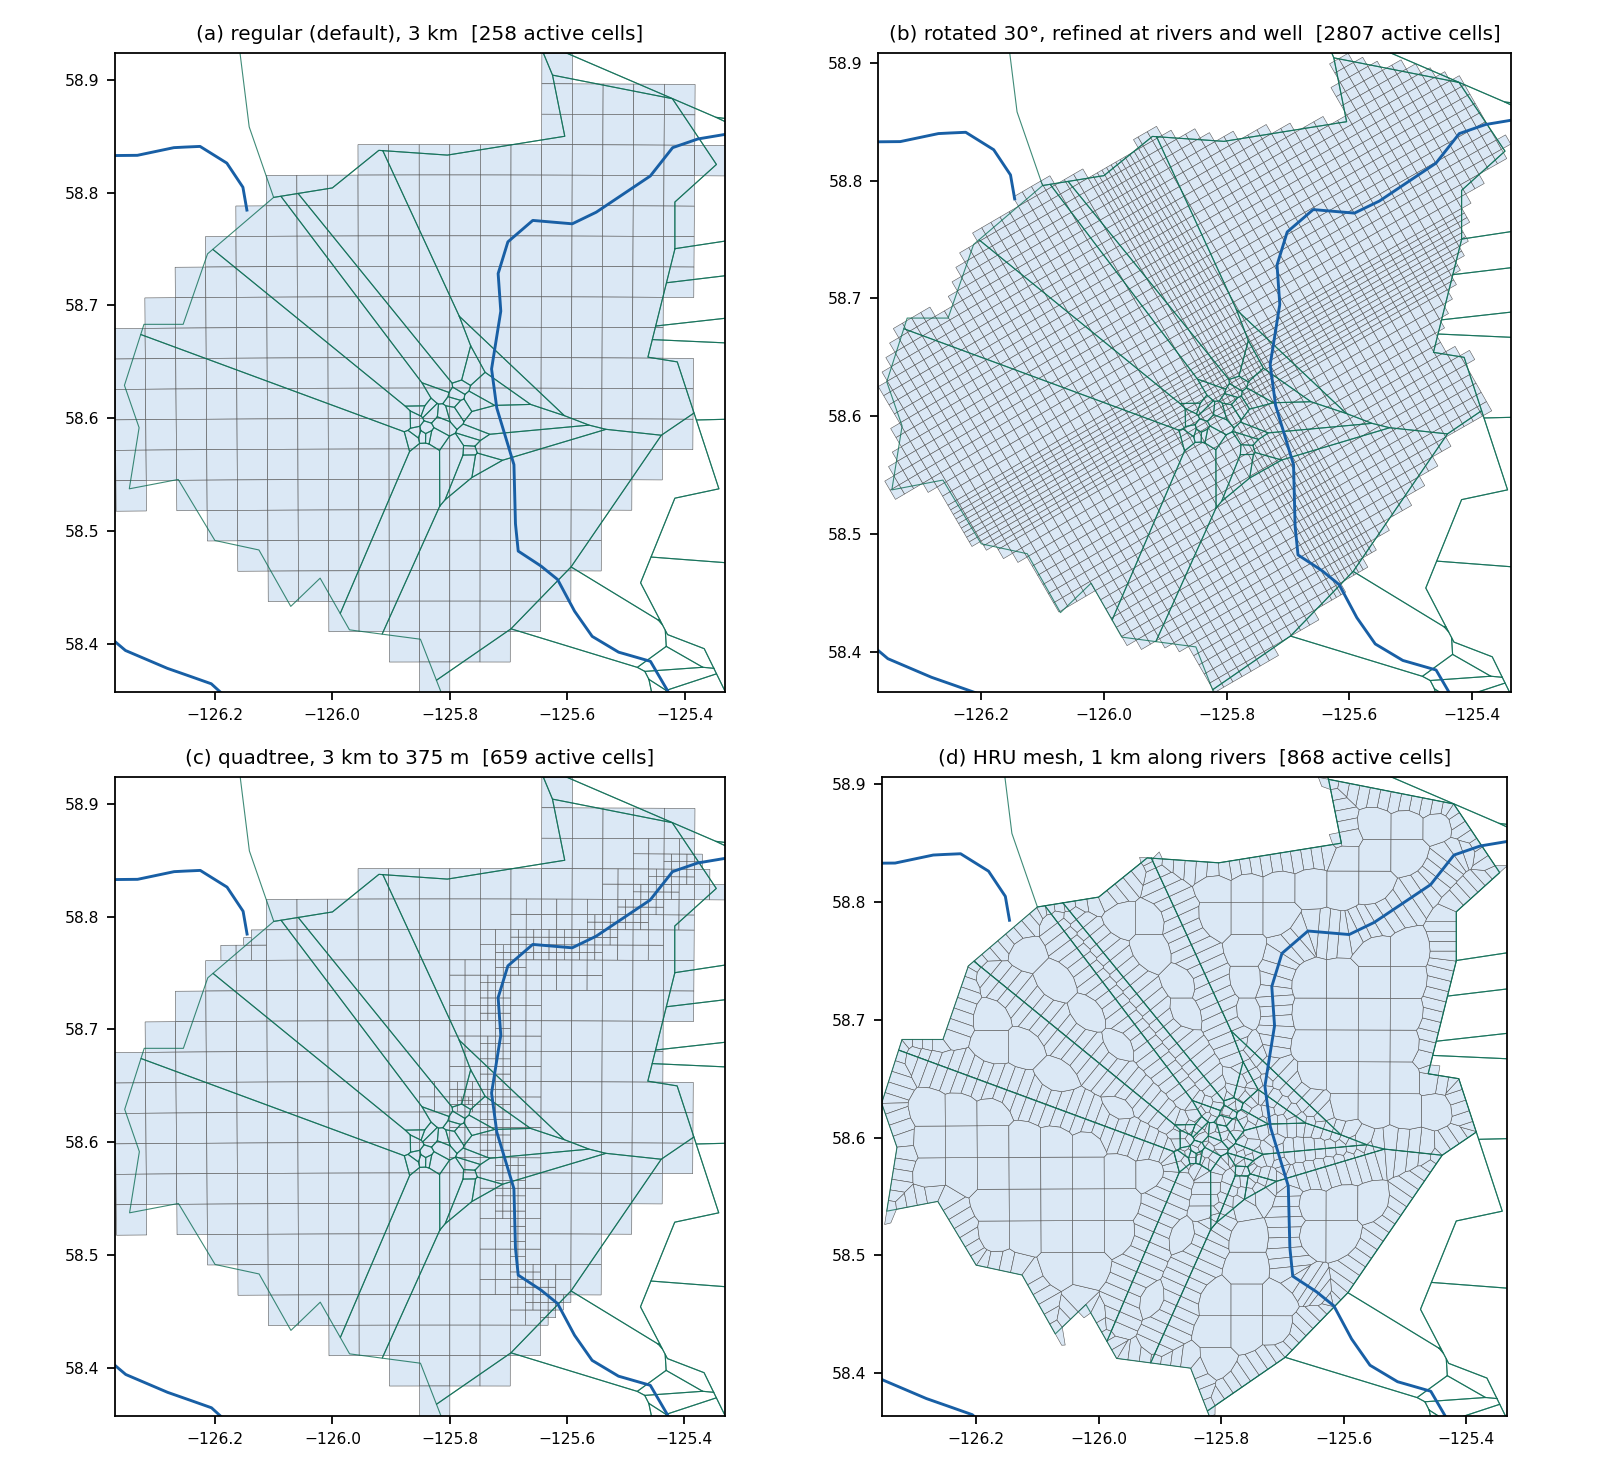
\includegraphics[width=0.78\linewidth]{figures/fig_grids.png}
\caption{The same model (Liard subbasin 52, HRU boundaries green, rivers blue) on four grids: (a) the default regular
grid; (b) rotated 30\textdegree{} and refined along rivers and around a well; (c) a quadtree refined along rivers and around the
well; (d) an HRU mesh whose cells follow HRU boundaries, with cells along the rivers.}\label{fig:ugrids}
\end{figure}
Figure~\ref{fig:ugrids} shows four of them.
\begin{table}[!htbp]\centering
\caption{Grid options and what to write in the \cmd{.rvg} file.}\label{tab:ugridtypes}
\begin{tabularx}{\linewidth}{P{0.25\linewidth}P{0.33\linewidth}Y}\toprule\hdr
Option & What to write & Use it when\\\midrule
Regular (default) & nothing, or \cmd{:GridType REGULAR} & a first model; uniform cells are enough\\
Rotated, refined & \cmd{:GridRotation 20}, \cmd{:GridRefinement RIVERS 1000} & a valley has a clear direction; finer rows and columns near rivers or wells\\
Quadtree & \cmd{:GridType QUADTREE} with \cmd{:GridRefinement} & fine cells only where they matter, few cells elsewhere\\
HRU mesh & \cmd{:GridType HRU\_MESH} & cells should follow HRU boundaries\\
Imported cells & \cmd{:GridType FILE}, \cmd{:GridFile cells.geojson} & a grid made elsewhere (FloPy, gridgen, ModelMuse, QGIS)\\
Layers by elevation & \cmd{:LayerConnection ELEVATION} & layers of neighbouring profiles should connect where they lie at the same elevation\\\bottomrule
\end{tabularx}
\end{table}
Start with the default grid and a cell size of a few kilometres. Refine where heads and exchanges change quickly: along
rivers that gain or lose much water, around pumping wells, around lakes and reservoirs, and in wetlands. Reference,
Section~\ref{R-sec:gridtypes}, describes each option. Every run writes \cmd{mf6/grid\_cells.geojson}, each cell as a
polygon ready to be joined with heads in QGIS.

\subsection{Choosing a grid for the Liard model}\label{sec:liardgrids}
The Liard model was run for two years on each grid option (Table~\ref{tab:liardgrids}). Every run keeps the water accounts
exact (MODFLOW residual about $10^{-11}$, no failed step, Raven's balance unchanged).
\begin{table}[!htbp]\centering
\caption{The Liard model (2 years) on each grid: active cells, run time on one core, Nash--Sutcliffe efficiency at 10BE004 /
10BE005 / 10BE010, mean seepage to Raven and mean net aquifer discharge to rivers [million m$^3$/d].}\label{tab:liardgrids}
\begin{tabular}{lrrcrr}\toprule\hdr
Grid & Cells & Time [s] & NSE & Seepage & Rivers\\\midrule
Regular 2 km (default) & 8\,840 & 40 & 0.728 / 0.861 / 0.635 & 9.48 & 0.82\\
Regular, rotated 20\textdegree, 1 km along rivers & 35\,058 & 220 & 0.726 / 0.861 / 0.638 & 9.92 & 0.66\\
Quadtree 2 km, 500 m along rivers & 16\,276 & 108 & 0.719 / 0.858 / 0.611 & 9.49 & 0.01\\
HRU mesh 2 km, 1 km along rivers & 14\,610 & 100 & 0.717 / 0.859 / 0.627 & 9.94 & 0.35\\
Regular 2 km, layers by elevation & 8\,840 & 41 & 0.666 / 0.859 / 0.606 & 4.11 & 0.49\\
\bottomrule\end{tabular}
\par\smallskip\footnotesize MODFLOW 6.8.1 (\cmd{tests/liard\_grids.py}); run times on one core of the test machine.
\end{table}
Streamflow hardly changes: total seepage is nearly the same on every grid, and the river exchange is a small part of the
flow at the gauges.

The net river exchange, however, depends on the size of the river cells: 0.82 million m$^3$/d with 2 km cells, 0.01 with
500 m cells. There are two reasons. The channel bed is placed at the lowest DEM value along the river in each cell,
which is lower in larger cells. And the head of a large cell averages the aquifer over a wider area around the river.
So calibrate the riverbed parameters (\cmd{RIVERBED\_K}, \cmd{:RiverBedDepth}) on the grid that will be used, and
compare models only at the same river-cell size.

Connecting layers by elevation halves the seepage here, because water in the upland till can flow directly into the
valley gravel where the two lie at the same elevation. That is a different conceptual model rather than a refinement. A
regular grid refined to 1 km along rivers has more than twice the cells of a quadtree with 500 m river cells, because its
refinement spans whole rows and columns.

\section{Starting heads}\label{sec:ustart}
Raven needs a head in every cell on the first day. It takes, in this order:
\begin{enumerate}
\item the heads of a hotstart file (\cmd{:GWHeads} in the \cmd{.rvc} file, Chapter~\ref{uch:restarts});
\item \cmd{:InitialGWHeads DEPTH\_BELOW\_SURFACE d} or \cmd{:InitialGWHeads ELEVATION z} in the \cmd{.rvc} file;
\item each profile's \cmd{INITIAL\_HEAD\_DEPTH} below the land surface.
\end{enumerate}
Guessed heads can be far from reality. \cmd{:GWInitialization STEADY\_STATE r} in the \cmd{.rvg} file first solves a
steady state with a recharge of $r$~mm/d over the area of the coupled HRUs, before Raven's first day. If that steady state
does not converge (for example when wells pump more than the aquifer can supply), Raven warns and starts from the initial
heads instead. Reference, Section~\ref{R-sec:init}, gives the details.

\section{Wells, monitoring wells and boundaries}\label{sec:uwells}
\begin{whattowrite}
\small In the \cmd{.rvg} file:
\begin{lstlisting}
:Wells
  :Attributes, NAME, LATITUDE, LONGITUDE, SCREEN_TOP, SCREEN_BOT
  1, PW_1, 59.27310, -124.73460, 1199.7, 1188.7
:EndWells
:ObservationWells
  :Attributes, NAME, LATITUDE, LONGITUDE, SCREEN_ELEV
  101, OW_NEAR, 59.27310, -124.73060, 1192.7
:EndObservationWells
:GeneralHeadBoundary   GHB1  boundary_line.geojson HEAD 1310.0 CONDUCTANCE 5000.0 LAYERS TOP
:SpecifiedHeadBoundary LAKE1 lake.geojson          HEAD 1312.0 LAYERS TOP
\end{lstlisting}
and in the \cmd{.rvt} file \cmd{:WellFlowRate 1 m3/d} (negative = pumping), \cmd{:BoundaryHead GHB1 m} (replaces
\cmd{HEAD}) and \cmd{:ObservationData GW\_HEAD 101 m}.
\end{whattowrite}
\begin{itemize}
\item \textbf{Wells} pump from (or inject into) the layers their screen crosses; the rate is split among the layers by
their transmissivity. A well rate series must cover the whole simulation, like every Raven forcing series. MODFLOW lowers
the rate of a well whose cell runs dry, and \cmd{GWBudget.csv} reports the specified and the actual rates.
\item \textbf{Monitoring wells} report the simulated head at their screen (\cmd{GWHeads.csv}) and are scored against
\cmd{:ObservationData GW\_HEAD} in \cmd{Diagnostics.csv}, like streamflow.
\item \textbf{Head-dependent boundaries} (\cmd{:GeneralHeadBoundary}) exchange water with a water body outside the model,
in proportion to the head difference. \textbf{Fixed-head boundaries} (\cmd{:SpecifiedHeadBoundary}) hold the head of their
cells.
\item A boundary is drawn in a GeoJSON file: polygons select the cells whose centre lies inside, lines the cells they
cross. \cmd{LAYERS ALL} (the default) places it in every active layer whose bottom lies below its head, \cmd{LAYERS TOP}
in the highest such layer. So the \cmd{HEAD} (or the \cmd{:BoundaryHead} series) must lie above the bottoms of the cells
it is to hold.
\item Two \cmd{:SpecifiedHeadBoundary} commands that select the same cell stop the run, naming both. General-head
boundaries may share cells.
\end{itemize}
Reference, Section~\ref{R-ch:wells}, gives the rules.

\section{Setting up your own model}\label{ch:ownmodel}
\subsection{A groundwater file to start from}
\begin{whattowrite}
\small
\begin{lstlisting}
# my.rvg - the groundwater file of a model Raven builds
:HRUGeometry        my_hrus.geojson   HRU_ID     # required
:RiverGeometry      my_rivers.geojson SubId      # river lines, subbasin ID field optional
:LandSurface        dem.tif                      # DEM
:BedrockSurface     bedrock.tif                  # or DEFAULT_BEDROCK_DEPTH of the profiles
:GridCellSize       1000.0                       # m
:GWInitialization   STEADY_STATE 0.5             # steady start, mean recharge [mm/d]
:HeadSaveFrequency  30
\end{lstlisting}
\end{whattowrite}
Add wells, monitoring wells, boundaries, wetlands and reservoirs as you need them. Reference, Section~\ref{R-ch:c6}, ends
with a groundwater file that uses most options.

\subsection{Checklist}
\begin{enumerate}
\item \textbf{HRU polygons.} Export the HRU polygons from your GIS or BasinMaker as GeoJSON in longitude/latitude
(EPSG:4326), or in their projection with \cmd{:InputCRS}, with a field holding the HRU ID used in the \cmd{.rvh} file.
\item \textbf{Maps.} A DEM and a bedrock (or aquifer-base) elevation map as GeoTIFF files or ESRI ASCII grids in
longitude/latitude (or in the projection of \cmd{:InputCRS}), in the same vertical datum. River lines as GeoJSON.
\item \textbf{Profiles.} Group your HRUs by the aquifer beneath them and write one profile per group; set
\cmd{AQUIFER\_PROFILE} in the \cmd{.rvh}.
\item \textbf{Recharge.} Decide which Raven flux is recharge (usually percolation from the deepest soil store) and send it
to \cmd{GROUNDWATER} for coupled HRUs only. Remove or restrict any process that drains \cmd{GROUNDWATER} there, and any
conceptual baseflow that would double-count groundwater.
\item \textbf{Grid size.} Choose $\Delta$ so that the smallest features you care about span a few cells, but the number of
active cells stays manageable (a few thousand to a few hundred thousand per layer).
\item \textbf{Start.} Use \cmd{:GWInitialization STEADY\_STATE} with the long-term average recharge, or a warm-up period.
\item \textbf{Check.} Read \cmd{GWModelSummary.txt} and run \cmd{tools\_audit.py} (Section~\ref{sec:uaudit}).
\item \textbf{Calibrate.} Use streamflow and monitoring-well heads (Section~\ref{ch:calib}).
\end{enumerate}

\subsection{Typical parameter values}
Typical values for aquifer materials are listed in Reference, Section~\ref{R-app:materials}, and typical ranges for every
aquifer class and profile parameter in Reference, Sections~\ref{R-app:class} and~\ref{R-app:profile}.

\subsection{How much of the water balance should groundwater take?}
In a coupled HRU, Raven's conceptual baseflow from deep stores is replaced by MODFLOW. Check after a first run that the
long-term baseflow (seepage plus aquifer discharge to rivers) is plausible, and that the aquifer is not steadily filling or
emptying (storage release near zero on average once spin-up is over).

\chapter{Coupling an existing MODFLOW~6 model}\label{uch:existing}
Many users already have a calibrated MODFLOW~6 model and want to connect it to a Raven model. In this mode Raven does
not build a groundwater model. It takes your model as it is: the grid, the layers, the conductivities, storage, wells,
boundaries, stress periods and solver settings. This chapter says what to write, what is supported and what is
refused. Reference, Chapter~\ref{R-ch:existing}, gives every rule. Workshop~4 couples a model in feet, on its own grid.

\begin{plain}
You give Raven your MODFLOW~6 model and tell it three things: where the model lies on the map, on what calendar date the
model's time starts, and which of the model's packages Raven should replace --- usually recharge and evaporation, which
Raven then supplies. Raven copies the model, makes a few changes to the copy, and runs the copy together with the Raven
model, one day at a time. Your own files are never changed.
\end{plain}

\section{What Raven changes, in a copy}
Raven links its HRUs to the model's \emph{top active layer} --- the highest layer that holds water at each location ---
and exchanges water there. Only three things change, and only in a working copy in \cmd{output/mf6/}:
\begin{enumerate}
\item the stress periods are split into Raven time steps;
\item the packages that Raven takes over (usually recharge and evapotranspiration) are switched off;
\item Raven's packages are added: \cmd{RCH\_RAVEN} (recharge from Raven) and \cmd{DRN\_RAVEN} (seepage back to Raven),
and, when the \cmd{.rvp} and \cmd{.rvg} files ask for them, \cmd{EVT\_RAVEN} (water-table evaporation), \cmd{SWX\_RAVEN}
(wetlands and lakes in Raven stores) and \cmd{RES\_RAVEN} (reservoir seepage).
\end{enumerate}
Raven copies the whole folder that holds the simulation file, so keep the model in a folder of its own. Old results
(\cmd{.hds}, \cmd{.cbc}, \cmd{.lst}, \cmd{.grb}, \cmd{.bud}, \cmd{.cbb}) are not copied.
\begin{figure}[!htbp]\centering% The working copy of an existing model (TikZ)
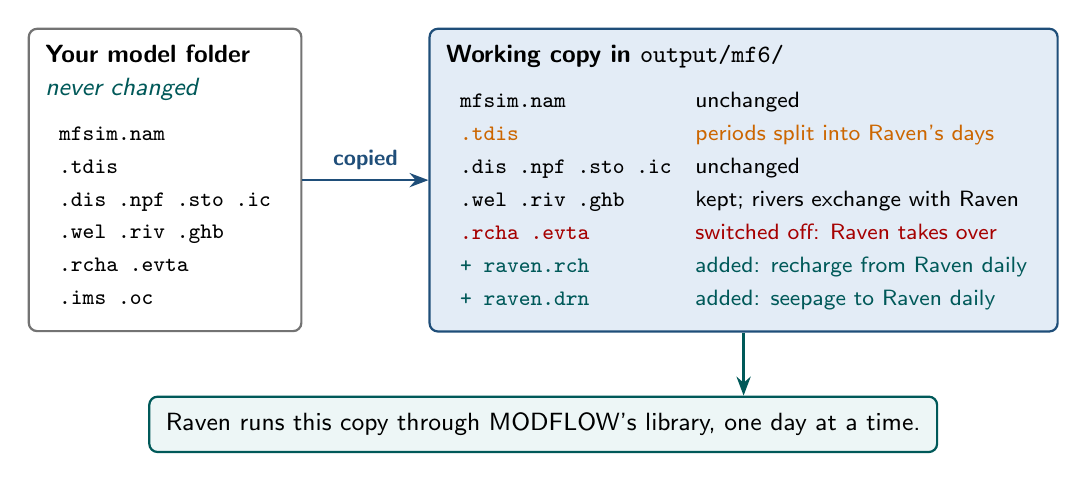
\begin{tikzpicture}[every node/.append style={execute at begin node={\hyphenpenalty=10000\exhyphenpenalty=10000}},font=\sffamily\small,arr/.style={-{Stealth[length=2.4mm]},line width=0.9pt}]
\node[draw=black!55,rounded corners=3pt,line width=0.8pt,fill=white,inner sep=6pt,align=left,anchor=north west] (L) at (0,0) {%
  \textbf{Your model folder}\\[1pt]{\itshape\color{teal!70!black}never changed}\\[5pt]
  {\footnotesize\ttfamily\begin{tabular}{l}mfsim.nam\\.tdis\\.dis .npf .sto .ic\\.wel .riv .ghb\\.rcha .evta\\.ims .oc\end{tabular}}};
\node[draw=brand,rounded corners=3pt,line width=0.8pt,fill=brandlight,inner sep=6pt,align=left,anchor=north west] (R) at ([xshift=16mm]L.north east) {%
  \textbf{Working copy in \texttt{output/mf6/}}\\[5pt]
  {\footnotesize\begin{tabular}{l@{\hspace{3mm}}l}
  \texttt{mfsim.nam} & unchanged\\
  \textcolor{orange!80!black}{\texttt{.tdis}} & \textcolor{orange!80!black}{periods split into Raven's days}\\
  \texttt{.dis .npf .sto .ic} & unchanged\\
  \texttt{.wel .riv .ghb} & kept; rivers exchange with Raven\\
  \textcolor{red!65!black}{\texttt{.rcha .evta}} & \textcolor{red!65!black}{switched off: Raven takes over}\\
  \textcolor{teal!70!black}{\texttt{+ raven.rch}} & \textcolor{teal!70!black}{added: recharge from Raven daily}\\
  \textcolor{teal!70!black}{\texttt{+ raven.drn}} & \textcolor{teal!70!black}{added: seepage to Raven daily}\\
  \end{tabular}}};
\draw[arr,brand] (L.east |- R.center) -- node[above,font=\sffamily\bfseries\footnotesize,text=brand]{copied} (R.west |- R.center);
\node[draw=teal!70!black,rounded corners=3pt,line width=0.8pt,fill=teal!7,inner sep=6pt,anchor=north] (B) at ([yshift=-8mm]current bounding box.south) {Raven runs this copy through MODFLOW's library, one day at a time.};
\draw[arr,teal!70!black] (R.south) -- (R.south |- B.north);
\end{tikzpicture}

\caption{Raven runs a working copy of the model. The copy differs from the original in three ways only; the original folder is never changed.}\label{fig:uworkcopy}
\end{figure}

\section{Example B}
\cmd{examples/Liard\_existing\_model/} holds a MODFLOW~6 model of the Liard coupled area, built independently of Raven:
a regular grid of 1.5~km cells rotated 15\textdegree{} in UTM zone 10N, four layers with spatially varying conductivity,
a one-day steady-state period followed by 24 monthly periods, two wells with seasonal pumping, 239 river cells carrying
their subbasin ID in an auxiliary variable, a head boundary at the outlet, and its own recharge and ET packages. This
\cmd{.rvg} file is all it takes:
\begin{whattowrite}
\small
\begin{lstlisting}
:HRUGeometry       Liard_HRUs_standin.geojson  HRU_ID
:MF6Simulation     model/mfsim.nam
:MF6CRS            EPSG:32610                  # the model's coordinates are UTM zone 10N
:MF6StartDate      1985-10-01                  # the calendar date of the model's time zero
:RavenTakesOver    RCH_MODEL EVT_MODEL         # Raven supplies recharge; the model's ET is replaced
:StreamPackage     RIV_STREAMS AUX SUBBASIN    # river cells carry their Raven subbasin ID
:SeepageToRaven    ON
\end{lstlisting}
\end{whattowrite}
The other Raven files are those of example~A; forcing and observations are read from \cmd{../Liard\_groundwater}, so keep
both folders side by side. Run it as example~A, from inside its folder. The two-year run takes about five minutes.

HRUs with an \cmd{AQUIFER\_PROFILE} in the \cmd{.rvh} file are coupled, as when Raven builds the model. The layers and
their properties come from the model's own files, so a profile needs no layers and no \cmd{:AquiferClasses} are needed.
Give each profile as \cmd{name, 0}; it then only marks the coupled HRUs and carries the exchange settings:
\begin{lstlisting}
:AquiferProfiles
  VALLEY_ALLUVIUM, 0                 # no layers: the model's own are used
  UPLAND_TILL,     0
:EndAquiferProfiles
:AquiferProfileParameters
  :Attributes,     SEEPAGE_LEAKANCE
  :Units,          1/d
  VALLEY_ALLUVIUM, 1.0
  UPLAND_TILL,     1.0
:EndAquiferProfileParameters
\end{lstlisting}
Of the profile parameters, \cmd{SEEPAGE\_LEAKANCE}, \cmd{SEEPAGE\_SMOOTHING\_DEPTH}, \cmd{RECHARGE\_DELAY} and
\cmd{EXTINCTION\_DEPTH} are used; the others are not. Layers listed in a profile are ignored, with a warning. Raven's
recharge must reach the \cmd{GROUNDWATER} store, exactly as when Raven builds the model (Chapter~\ref{uch:build}).

\section{Telling Raven where the model is}
MODFLOW model files do not say where on Earth the model is. Give exactly one of these:
\begin{itemize}
\item \textbf{\cmd{:MF6CRS} (recommended)}: the model's map projection, usually as an EPSG code (\cmd{EPSG:32610} is UTM
zone 10 North), or a Transverse Mercator, Albers or Lambert projection by its parameters. Raven reads the cell outlines
from the model and places them on the map. No external software is needed.
\item \textbf{\cmd{:MF6GridFile}}: a GeoJSON file of the top-layer cells, numbered from 1 in the model's order, as GIS
software exports it. Raven checks that the polygons are the model's cells.
\item \textbf{\cmd{:OverlapWeights}}: a table of HRU, cell and the share of the cell the HRU covers, prepared outside Raven.
No HRU polygons are needed, but monitoring wells cannot be located.
\end{itemize}
Each coupled HRU is then linked to the top active cell of every column it overlaps. \cmd{GWModelSummary.txt} reports how
much of the coupled HRUs' area lies on active model cells (99.74\% in example~B).

\section{Time}
MODFLOW models divide time into stress periods. Raven keeps the model's stress periods and their dates, and splits each
period into Raven time steps, so the model's own changes --- a well pumping harder in summer, a boundary level changing
--- still happen on their dates.
\begin{itemize}
\item \cmd{:MF6StartDate} is the calendar date on which the model's time starts (with its time of day when that is not
midnight). It is required.
\item Each stress period must hold a whole number of Raven time steps, and Raven's run may not go past the end of the
model. Otherwise the run stops with a message. Steady-state periods stay steady-state.
\item A steady-state model (one period, no storage) is stretched over Raven's run: every Raven step is a steady-state
solution with that step's recharge, and the storage column of \cmd{GWBudget.csv} stays zero. Raven may then start on any
date from \cmd{:MF6StartDate} on.
\end{itemize}

\section{Units}
Length units (metres, feet, centimetres) are read from the model's discretization package, and time units (seconds to
years) from its time discretization. Heads, flows, rates, conductances and coordinates are converted at the interface.
Raven's outputs are always in metres and days.

\section{The model's packages}
\begin{itemize}
\item \textbf{Recharge, evapotranspiration and UZF packages} must each be named in \cmd{:RavenTakesOver} (removed; Raven
supplies recharge) or in \cmd{:KeepPackages} (they stay). An undeclared one stops the run, so recharge is never counted
twice.
\item \textbf{The stream package} (\cmd{:StreamPackage}): a RIV, DRN or GHB package whose flows go to Raven's reaches,
either to the subbasin in an auxiliary variable (\cmd{AUX}, default \cmd{SUBBASIN}) or to the subbasin of the cell's
dominant HRU (\cmd{DOMINANT\_HRU}).
\item \textbf{Seepage} (\cmd{:SeepageToRaven ON}): \cmd{DRN\_RAVEN} at the top of the top active cell of coupled columns
returns groundwater that reaches the surface to Raven.
\item \textbf{Everything else is kept unchanged}: wells, head boundaries, drains, lakes, streamflow routing, the water
mover (movers to or from a package Raven takes over are removed), skeletal storage and compaction. Their flows enter
the balance check (\cmd{GWBudget.csv}, column \emph{other model packages}).
\item \textbf{The model's solver} (\cmd{.ims}) and output control are kept. The first coupled step is often the hardest
--- a steady-state period solved from the model's starting heads with Raven's recharge --- so allow at least 500 outer
iterations (\cmd{OUTER\_MAXIMUM}).
\end{itemize}
Reference, Table~\ref{R-tab:extpkgs}, gives the treatment of every package.

\section{What is supported, and what is refused}\label{sec:uextrefused}
Raven refuses a model it cannot couple safely, with a message that names the problem and the fix. The main cases are in
Table~\ref{tab:uextrefused}; Reference, Section~\ref{R-sec:extlimits} and the safeguards before it, list them all.
\begin{table}[!htbp]\centering
\caption{Existing models: what is supported and what is refused.}\label{tab:uextrefused}
\begin{tabularx}{\linewidth}{P{0.38\linewidth}Y}\toprule\hdr
Model feature & Why it is refused, or how it is handled\\\midrule
DIS and DISV grids & supported\\
DISU grids & not supported\\
more than 5 million cells per layer & refused: the limit of the grids Raven builds\\
more than one model, or exchanges & refused: Raven couples one groundwater-flow model and books only its water\\
transport, energy or particle-tracking models (\cmd{GWT6}, \cmd{GWE6}, \cmd{PRT6}) & refused: run them separately, from the heads and budget files of the Raven run\\
more than one solution & refused: Raven drives the one model's solution\\
adaptive time stepping (\cmd{ATS6}) & refused: Raven needs fixed time steps\\
an undeclared recharge, ET or UZF package & refused, so that recharge is never counted twice\\
\cmd{EXTINCTION\_DEPTH} in a profile while the model keeps an EVT or UZF package & refused\\
a stream package that sends water through the mover & refused: Raven would take the same water from the aquifer twice\\
options of the generated mode in the \cmd{.rvg} (\cmd{:GridCellSize}, \cmd{:Wells}, \cmd{:LandSurface}, \dots) & refused\\
a Raven calendar other than Gregorian & refused: the dates of the two models are compared day by day\\
a Raven start before \cmd{:MF6StartDate} & refused\\\bottomrule
\end{tabularx}
\end{table}

\section{Starting later, and restarts}\label{sec:uextrestart}
Raven may start later than the model's time zero: when a run is continued from \cmd{solution.rvc}, or begins part-way
through the model. Raven then drops the stress periods already simulated from the working copy, shortens the period that
holds Raven's start, and renumbers the periods; the new first period takes the inputs that were in force on Raven's start
date. Times of time series (\cmd{TS6}) are shifted to match. Figure~\ref{fig:uperiods} shows an example.
\begin{figure}[!htbp]\centering% Stress periods, Raven's days and a restart after 40 days (TikZ; 1 mm per day)
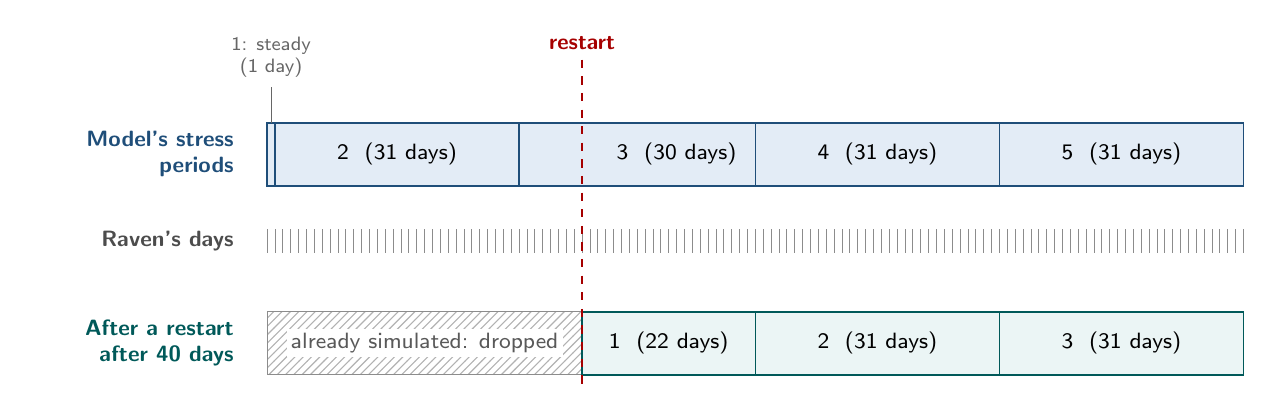
\begin{tikzpicture}[every node/.append style={execute at begin node={\hyphenpenalty=10000\exhyphenpenalty=10000}},x=1mm,y=1mm,font=\sffamily\footnotesize,
  rowlab/.style={anchor=east,align=right,text width=25mm,font=\sffamily\footnotesize\bfseries},
  per/.style={draw=brand,fill=brandlight,line width=0.6pt},
  new/.style={draw=teal!70!black,fill=teal!8,line width=0.6pt}]
% row 1: the model's stress periods (1 steady day, then 31, 30, 31, 31 days)
\node[rowlab,text=brand] at (-3,0) {Model's stress\\periods};
\draw[per] (0,-4) rectangle (1,4);
\foreach \a/\b/\t/\lx in {1/32/{2 \ (31 days)}/16.5, 32/62/{3 \ (30 days)}/52, 62/93/{4 \ (31 days)}/77.5, 93/124/{5 \ (31 days)}/108.5}{
  \draw[per] (\a,-4) rectangle (\b,4); \node at (\lx,0) {\t};}
\draw[black!60] (0.5,4) -- (0.5,8.5) node[above,align=center,font=\sffamily\scriptsize] {1: steady\\(1 day)};
% row 2: Raven's days
\node[rowlab,text=black!70] at (-3,-11) {Raven's days};
\foreach \d in {0,...,124}{\draw[black!45,line width=0.3pt] (\d,-12.5) -- (\d,-9.5);}
% row 3: after a restart after 40 days
\node[rowlab,text=teal!70!black] at (-3,-24) {After a restart\\after 40 days};
\draw[black!45,fill=black!6,pattern=north east lines,pattern color=black!30] (0,-28) rectangle (40,-20);
\node[fill=white,inner sep=1.5pt,text=black!65] at (20,-24) {already simulated: dropped};
\foreach \a/\b/\t in {40/62/{1 \ (22 days)}, 62/93/{2 \ (31 days)}, 93/124/{3 \ (31 days)}}{
  \draw[new] (\a,-28) rectangle (\b,-20); \node at ({(\a+\b)/2},-24) {\t};}
% the restart
\draw[red!65!black,dashed,line width=0.9pt] (40,12) -- (40,-30);
\node[above,text=red!65!black,font=\sffamily\bfseries\footnotesize] at (40,12) {restart};
\end{tikzpicture}

\caption{Top: a model with a one-day steady period followed by periods of 31, 30, 31 and 31 days, and Raven's days. Bottom: after a restart 40 days into the model, the time already simulated is dropped, period~3 keeps its last 22 days, and the periods are renumbered; each keeps its own well rates and boundary levels.}\label{fig:uperiods}
\end{figure}

Some packages cannot follow such a start, because their settings build on one another. A later start stops when the
model has time-array series (\cmd{TAS6}), time-varying conductivity or storage (\cmd{TVK6}, \cmd{TVS6}), or array-based or
advanced packages (SFR, LAK, MAW, UZF) with several period entries before Raven's start. Raven must then start at
\cmd{:MF6StartDate}.

A restart carries only the heads. So a restarted run reproduces a continuous one only when the model keeps no package
with a state of its own. In MODFLOW~6.8.1 those are LAK (lake stages), MAW (well heads), UZF (unsaturated-zone water
content), CSUB (stresses) and SFR with the \cmd{STORAGE} option. A restart (\cmd{:GWHeads}) of a model that keeps any of
them stops, naming it. Then remove \cmd{:GWHeads} from the \cmd{.rvc} file, so that every package starts from its input,
or simulate the whole period in one run. Reference, Section~\ref{R-sec:existingtime}, gives the rules.

\section{Rivers in an existing model}
The model's stream package keeps its own stage and conductance. Unlike the river cells Raven builds, it has no supply
limit, so a losing reach can take more than its channel holds. The part the channel cannot supply is carried to the next
step and taken then, and it is exactly accounted (\emph{river loss carried to next step} in \cmd{GWBudget.csv}).

Example~B does this for months: \cmd{river loss carried max} of the audit tool is about $1.06\times10^{8}$~m$^3$, on 271
of the 731 days from the first day, and the carry is repaid by the end of the run (\cmd{river loss carried at end} 0).
Raven warns on the first ten such steps.

\section{Outputs, and checking the calibration}
All the outputs of Chapter~\ref{uch:outputs} are written. \cmd{GWModelSummary.txt} also describes the coupling:
\begin{lstlisting}
existing model        : GWF_LIARD in model/mfsim.nam (DIS, 4 layers x 11466 cells per layer; metres, days)
cells linked by       : cell outlines from MODFLOW, Transverse Mercator (...)
packages taken over   : RCH_MODEL EVT_MODEL
packages in balance   : GHB_OUTLET WEL_PUMPS
stream package        : RIV_STREAMS (subbasin from auxiliary SUBBASIN)
HRU coverage          : 99.74% of the coupled HRUs' polygon area lies on active model cells
\end{lstlisting}
In \cmd{GWHRUState.csv} the water-table depth is measured from the top of the model's top active cell, which stands for
the land surface. The model keeps its own output control: for MODFLOW's budget file, add \cmd{BUDGET FILEOUT} and
\cmd{SAVE BUDGET} to its OC file.

Replacing a calibrated recharge package with Raven's recharge changes the model's water budget. Compare the coupled heads
and budget with a run of the original model before using the results. Large differences mean that Raven's recharge, or
the recharge the model was calibrated with, needs attention.

\chapter{The exchanges in plain terms}\label{uch:exchanges}
Raven and MODFLOW exchange water in eight ways, and in a ninth when the soil zone is coupled
(Table~\ref{tab:uexchanges}). This chapter says what each exchange does, what controls it and what to write. Reference,
Chapter~\ref{R-ch:c4}, gives the equations, the safeguards and worked examples with numbers.

Figure~\ref{fig:uexch} shows where each exchange crosses between Raven and MODFLOW, and the table below lists them.
\begin{table}[!htbp]\centering
\caption{The exchanges between Raven and MODFLOW, and what switches them on.}\label{tab:uexchanges}\small
\begin{tabularx}{\linewidth}{P{0.2\linewidth}P{0.17\linewidth}P{0.2\linewidth}Y}\toprule\hdr
Exchange & Direction & Raven side & Switched on by\\\midrule
Recharge & Raven $\to$ aquifer & \cmd{GROUNDWATER} & always\\
Seepage & aquifer $\to$ Raven & lowest soil layer & always (existing model: \cmd{:SeepageToRaven ON})\\
Soil zone & both & soil-zone layers & \cmd{:SoilZone PHYSICAL}\\
Rivers & both & reach inflow & \cmd{:RiverGeometry} (existing model: \cmd{:StreamPackage})\\
Water-table ET & aquifer $\to$ air & unmet PET & \cmd{EXTINCTION\_DEPTH}~$>0$\\
Wetlands, lakes & both & HRU store & \cmd{:SurfaceWaterExchange}\\
Reservoirs & both & reservoir seepage & \cmd{:ReservoirExchange}\\
Wells & out (or in) & time series & \cmd{:Wells}\\
Boundaries & both & time series & \cmd{:GeneralHeadBoundary}, \cmd{:SpecifiedHeadBoundary}\\\bottomrule
\end{tabularx}\end{table}
\begin{figure}[!htbp]\centering% The exchanges between Raven and MODFLOW (both volumes of the manual)
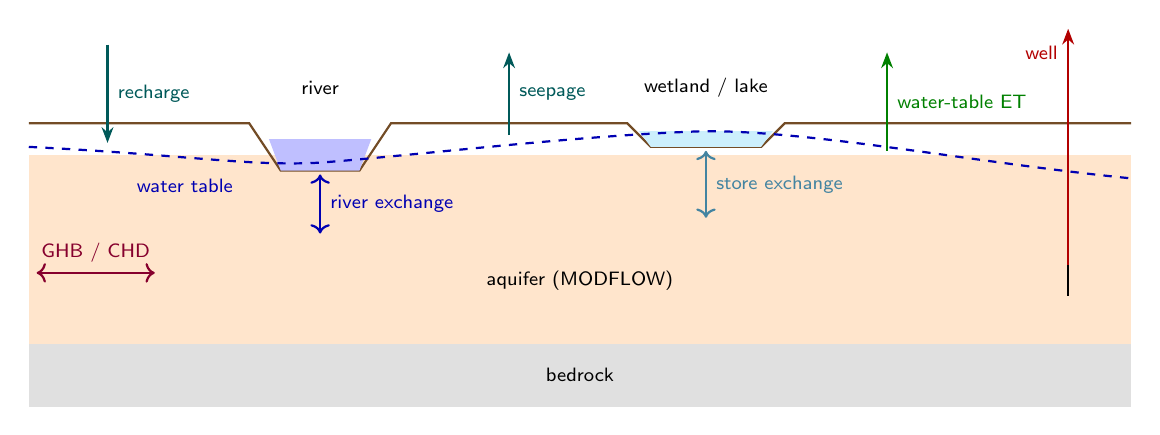
\begin{tikzpicture}[x=1cm,y=1cm,lab/.style={font=\scriptsize,align=center},ar/.style={-{Stealth[length=2mm]},thick}]
\fill[orange!20] (0,0.8) rectangle (14,3.2); \fill[black!12] (0,0) rectangle (14,0.8);
\draw[thick,brown!60!black] (0,3.6) -- (2.8,3.6) -- (3.2,3.0) -- (4.2,3.0) -- (4.6,3.6) -- (7.6,3.6) -- (7.9,3.3) -- (9.3,3.3) -- (9.6,3.6) -- (14,3.6);
\fill[blue!25] (3.05,3.4) -- (4.35,3.4) -- (4.2,3.0) -- (3.2,3.0) -- cycle; \node[lab] at (3.7,4.05) {river};
\fill[cyan!20] (7.75,3.5) -- (9.45,3.5) -- (9.3,3.3) -- (7.9,3.3) -- cycle; \node[lab] at (8.6,4.05) {wetland / lake};
\draw[dashed,blue!70!black,thick] (0,3.3) .. controls (2,3.2) and (2.8,3.05) .. (3.7,3.1) .. controls (5,3.2) and (7,3.45) .. (8.6,3.5) .. controls (10,3.5) and (12,3.1) .. (14,2.9);
\node[lab,blue!70!black,anchor=west] at (1.25,2.8) {water table};
\draw[ar,teal!70!black] (1.0,4.6) -- node[lab,right]{recharge} (1.0,3.35);
\draw[ar,teal!70!black] (6.1,3.45) -- node[lab,right]{seepage} (6.1,4.5);
\draw[ar,blue!70!black,<->] (3.7,2.95) -- node[lab,right]{river exchange} (3.7,2.2);
\draw[ar,cyan!60!black,<->] (8.6,3.25) -- node[lab,right]{store exchange} (8.6,2.4);
\draw[ar,green!50!black] (10.9,3.25) -- node[lab,right]{water-table ET} (10.9,4.5);
\draw[thick] (13.2,4.7) -- (13.2,1.4); \draw[ar,red!70!black] (13.2,1.8) -- node[lab,left,pos=0.9]{well} (13.2,4.8);
\draw[ar,purple!70!black,<->] (0.1,1.7) -- node[lab,above]{GHB / CHD} (1.6,1.7);
\node[lab] at (7,1.6) {aquifer (MODFLOW)}; \node[lab] at (7,0.4) {bedrock};
\end{tikzpicture}

\caption{The exchanges between Raven (above the water table) and MODFLOW (below). Reservoir seepage works like the store
exchange, through Raven's reservoir seepage law.}\label{fig:uexch}
\end{figure}

\section{Recharge}\label{sec:urecharge}
Figure~\ref{fig:ulinking} shows how an HRU's water is shared among the cells under it.
\begin{figure}[!htbp]\centering% HRU over grid cells with its share in each cell (generated by make_tikz_linking.py; shares computed from the shapes)
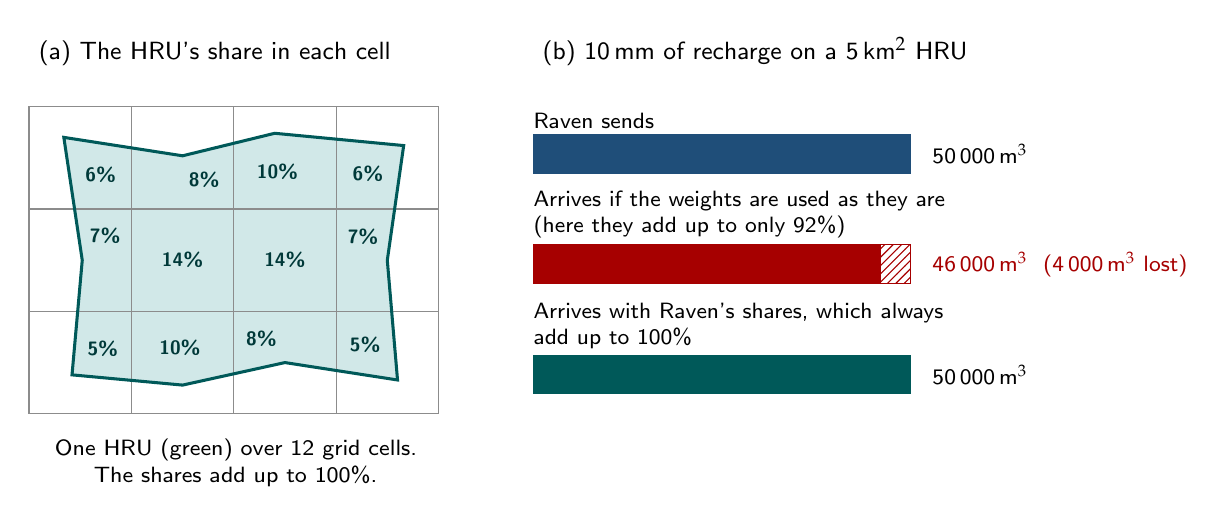
\begin{tikzpicture}[x=1mm,y=1mm,font=\sffamily\footnotesize,every node/.append style={execute at begin node={\hyphenpenalty=10000\exhyphenpenalty=10000}}]
\node[anchor=south west,font=\sffamily\small] at (0,43) {(a) The HRU's share in each cell};
\fill[teal!18] (5.46,4.94) -- (19.50,3.64) -- (32.50,6.50) -- (46.80,4.29) -- (45.50,19.50) -- (47.58,34.06) -- (31.20,35.62) -- (19.50,32.76) -- (4.42,35.10) -- (6.76,19.50) -- cycle;
\draw[black!45,line width=0.4pt] (0,0) rectangle (13,13);
\draw[black!45,line width=0.4pt] (0,13) rectangle (13,26);
\draw[black!45,line width=0.4pt] (0,26) rectangle (13,39);
\draw[black!45,line width=0.4pt] (13,0) rectangle (26,13);
\draw[black!45,line width=0.4pt] (13,13) rectangle (26,26);
\draw[black!45,line width=0.4pt] (13,26) rectangle (26,39);
\draw[black!45,line width=0.4pt] (26,0) rectangle (39,13);
\draw[black!45,line width=0.4pt] (26,13) rectangle (39,26);
\draw[black!45,line width=0.4pt] (26,26) rectangle (39,39);
\draw[black!45,line width=0.4pt] (39,0) rectangle (52,13);
\draw[black!45,line width=0.4pt] (39,13) rectangle (52,26);
\draw[black!45,line width=0.4pt] (39,26) rectangle (52,39);
\draw[teal!70!black,line width=1.1pt] (5.46,4.94) -- (19.50,3.64) -- (32.50,6.50) -- (46.80,4.29) -- (45.50,19.50) -- (47.58,34.06) -- (31.20,35.62) -- (19.50,32.76) -- (4.42,35.10) -- (6.76,19.50) -- cycle;
\node[font=\sffamily\bfseries\scriptsize,text=teal!45!black,inner sep=0.5pt] at (9.37,8.21) {5\%};
\node[font=\sffamily\bfseries\scriptsize,text=teal!45!black,inner sep=0.5pt] at (9.67,22.57) {7\%};
\node[font=\sffamily\bfseries\scriptsize,text=teal!45!black,inner sep=0.5pt] at (9.10,30.37) {6\%};
\node[font=\sffamily\bfseries\scriptsize,text=teal!45!black,inner sep=0.5pt] at (19.17,8.35) {10\%};
\node[font=\sffamily\bfseries\scriptsize,text=teal!45!black,inner sep=0.5pt] at (19.50,19.50) {14\%};
\node[font=\sffamily\bfseries\scriptsize,text=teal!45!black,inner sep=0.5pt] at (22.24,29.67) {8\%};
\node[font=\sffamily\bfseries\scriptsize,text=teal!45!black,inner sep=0.5pt] at (29.53,9.47) {8\%};
\node[font=\sffamily\bfseries\scriptsize,text=teal!45!black,inner sep=0.5pt] at (32.50,19.50) {14\%};
\node[font=\sffamily\bfseries\scriptsize,text=teal!45!black,inner sep=0.5pt] at (31.56,30.78) {10\%};
\node[font=\sffamily\bfseries\scriptsize,text=teal!45!black,inner sep=0.5pt] at (42.70,8.71) {5\%};
\node[font=\sffamily\bfseries\scriptsize,text=teal!45!black,inner sep=0.5pt] at (42.43,22.47) {7\%};
\node[font=\sffamily\bfseries\scriptsize,text=teal!45!black,inner sep=0.5pt] at (43.05,30.47) {6\%};
\node[anchor=north,align=center,text width=50mm] at (26,-2) {One HRU (green) over 12 grid cells.\\The shares add up to 100\%.};
\node[anchor=south west,font=\sffamily\small] at (64,43) {(b) 10\,mm of recharge on a 5\,km$^2$ HRU};
\node[anchor=south west,align=left,inner sep=0pt] at (64,36.2) {Raven sends};
\fill[brand] (64,30.5) rectangle (112,35.5);
\node[anchor=west] at (113.5,33) {50\,000\,m$^3$};
\node[anchor=south west,align=left,inner sep=0pt] at (64,22.2) {Arrives if the weights are used as they are\\(here they add up to only 92\%)};
\fill[red!65!black] (64,16.5) rectangle (108.16,21.5);
\draw[red!65!black,pattern=north east lines,pattern color=red!65!black] (108.16,16.5) rectangle (112,21.5);
\node[anchor=west,text=red!65!black] at (113.5,19) {46\,000\,m$^3$ \ (4\,000\,m$^3$ lost)};
\node[anchor=south west,align=left,inner sep=0pt] at (64,8.2) {Arrives with Raven's shares, which always\\add up to 100\%};
\fill[teal!70!black] (64,2.5) rectangle (112,7.5);
\node[anchor=west] at (113.5,5) {50\,000\,m$^3$};
\end{tikzpicture}

\caption{Sharing an HRU's water among cells. (a) Raven computes the HRU's share in each cell from the shapes, and the shares add up to 100\%. (b) If the shares added up to only 92\%, 8\% of the water would be lost; because Raven's shares always add up to 100\%, every cubic metre arrives.}\label{fig:ulinking}
\end{figure}
Recharge is whatever Raven's processes put into the \cmd{GROUNDWATER} store of a coupled HRU during a step. Its volume is
that depth of water times the HRU's area in the \cmd{.rvh} file. Raven spreads it over the cells under the HRU, in
proportion to how much of the HRU lies in each cell, and hands it to MODFLOW the same step. Recharge that falls on
fixed-head cells goes to the fixed heads and is reported apart (\emph{recharge onto CHD cells}).

Recharge is therefore controlled by Raven's own process choices: percolation, infiltration, frozen ground and so on. The
coupling adds no control of its own.

\paragraph{Optional delay.} The profile parameter \cmd{RECHARGE\_DELAY} $\tau$ (days) holds recharge in a linear store
before it reaches MODFLOW. Each day the store releases the share $1-e^{-1/\tau}$ of its water; with $\tau=60$~d that is
1.65\% a day, and 63\% of a pulse has arrived after 60 days. With \cmd{:SoilZone PHYSICAL}, use an unsaturated column
(\cmd{:SoilZoneVadose LAG}) instead.

\section{Seepage back to Raven}\label{sec:useepage}
Figure~\ref{fig:ucurves} shows how four of the exchanges respond: a delayed recharge, the seepage near the land surface, a river, and evaporation from the water table.
\begin{figure}[!htbp]\centering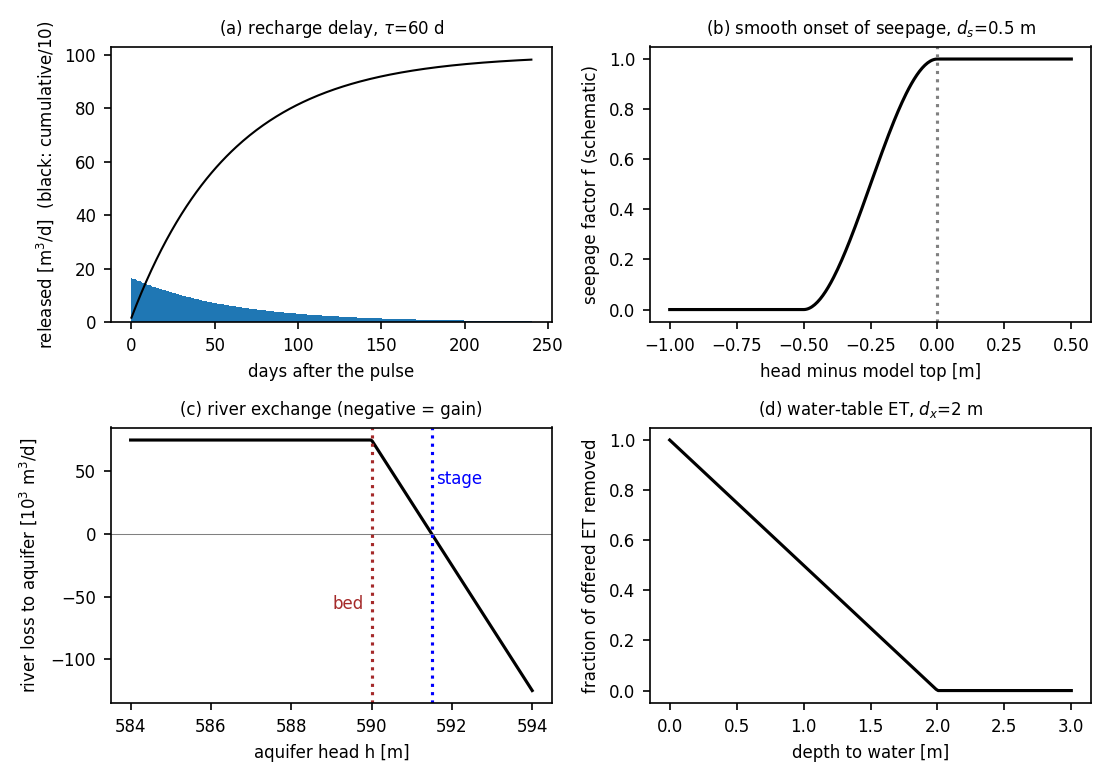
\includegraphics[width=\linewidth]{figures/fig_curves.png}
\caption{How four exchanges respond. (a) Recharge held in a delay reservoir reaches the aquifer gradually after a pulse of 1\,000~m$^3$. (b) Seepage starts as the water table nears the model top. (c) A river gains water when the aquifer head is above its stage and loses it when the head is below, at a limited rate once the water table drops below the river bed. (d) Evaporation from the water table is largest at the surface and stops at the extinction depth.}\label{fig:ucurves}
\end{figure}
Where the water table reaches the model top, groundwater flows out through a drain at the top of each cell. The drain
starts to flow \cmd{SEEPAGE\_SMOOTHING\_DEPTH} (default 0.5~m) below the top, and its strength is
\cmd{SEEPAGE\_LEAKANCE} (default 1/d) times the cell area. It is a strong outlet, so wherever the aquifer is full the water
table settles very close to the surface.

The seepage of a cell is returned to the HRUs above it, in proportion to their overlap, into the store named by
\cmd{:SeepageReturnTo}: by default the lowest soil layer, and \cmd{SURFACE\_WATER} for HRUs without soil. Raven's own
processes then carry it on, for example as baseflow to the river.

\section{Rivers}\label{sec:urivers}
Figure~\ref{fig:uriver} shows a river cell.
\begin{figure}[!htbp]\centering
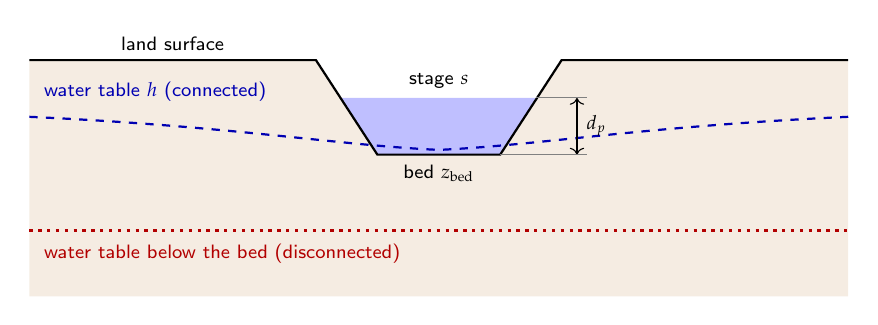
\begin{tikzpicture}[x=1.3cm,y=1.2cm,lab/.style={font=\scriptsize}]
\fill[brown!15] (-4,0) -- (4,0) -- (4,2.5) -- (1.2,2.5) -- (0.6,1.5) -- (-0.6,1.5) -- (-1.2,2.5) -- (-4,2.5) -- cycle;
\fill[blue!25] (-0.95,2.1) -- (0.95,2.1) -- (0.6,1.5) -- (-0.6,1.5) -- cycle;
\draw[thick] (-4,2.5) -- (-1.2,2.5) -- (-0.6,1.5) -- (0.6,1.5) -- (1.2,2.5) -- (4,2.5);
\draw[dashed,blue!70!black,thick] (-4,1.9) .. controls (-2,1.8) and (-1,1.6) .. (0,1.55) .. controls (1,1.6) and (2,1.8) .. (4,1.9);
\node[lab,blue!70!black,anchor=west] at (-3.95,2.17) {water table $h$ (connected)};
\draw[dotted,red!70!black,very thick] (-4,0.7) -- (4,0.7); \node[lab,red!70!black,anchor=west] at (-3.95,0.45) {water table below the bed (disconnected)};
\draw[<->] (1.35,1.5) -- (1.35,2.1); \node[lab,right] at (1.35,1.8) {$d_p$};
\draw[gray,thin] (0.6,1.5) -- (1.45,1.5); \draw[gray,thin] (0.95,2.1) -- (1.45,2.1);
\node[lab] at (0,2.28) {stage $s$}; \node[lab] at (0,1.3) {bed $z_{\mathrm{bed}}$};
\node[lab,anchor=south] at (-2.6,2.5) {land surface};
\end{tikzpicture}

\caption{A river cell. The river's stage is its bed plus the channel depth Raven computes. While the water table is above the bed, water flows toward the lower of the two levels; once the water table drops below the bed, the river loses water at a rate that no longer grows as the water table falls.}\label{fig:uriver}
\end{figure}
Rivers exchange water with the aquifer in both directions. A \emph{gaining} river receives groundwater; a \emph{losing}
river leaks into the aquifer. Raven places a river cell (MODFLOW's RIV package) in every cell crossed by a river line of
\cmd{:RiverGeometry}. The exchange of a river cell is
\[
q = C\,(s-h),
\]
where $q$ is the flow from the river into the aquifer [m$^3$/d], $s$ the river level, $h$ the head of the cell, and $C$
the riverbed conductance: the riverbed conductivity \cmd{RIVERBED\_K} times the river's width and length in the cell,
divided by the riverbed thickness \cmd{RIVERBED\_THICKNESS}. When the head falls below the riverbed, the loss stops
growing: $h$ is replaced by the bed elevation.

\begin{itemize}
\item \textbf{The riverbed} lies one bankfull depth of Raven's channel (at its reference flow) below the lowest DEM value
along the river in the cell, or \cmd{:RiverBedDepth} metres below it.
\item \textbf{The river level} each day is the bed plus Raven's channel depth at the start of the day, never above the
land surface.
\item \textbf{A gain} is added to the subbasin's inflow for the day, so it passes Raven's routing like other runoff.
\item \textbf{A loss} (the \emph{river-loss take}) is taken from the subbasin's own inflow, then from the flow entering the
reach from upstream, then from the reach's outflow. The outflow leaving the watershed is lower by exactly the water
MODFLOW receives.
\end{itemize}
\begin{example}[: a river cell]
Riverbed conductivity 0.5~m/d, riverbed 1~m thick, river 40~m wide, 2\,500~m of river in the cell:
$C=0.5\times40\times2\,500/1=50\,000$~m$^2$/d. Bed at 590~m, river 1.5~m deep, so the river level is 591.5~m.
With the water table at 590.8~m the river loses $50\,000\times0.7=35\,000$~m$^3$/d to the aquifer. With the water table
at 592.0~m it gains 25\,000~m$^3$/d. With the water table at 585~m, below the bed, it loses
$50\,000\times1.5=75\,000$~m$^3$/d, and no more however low the water table falls.
\end{example}

\paragraph{A river cannot lose more than it carries.} Raven limits the conductance of each river cell every day, so that
the largest possible loss is no more than the cell's share (by river length) of the flow in the reach at the start of
the day. Only a reach whose flow stops within the step can leave part of its loss unpaid; that part is carried to the next
step (\emph{river loss carried to next step}, normally 0; Raven warns). An existing model's stream package has no such
limit (Chapter~\ref{uch:existing}).

\begin{inpractice}
Calibrate \cmd{RIVERBED\_K} and \cmd{:RiverBedDepth} on the grid you will use: the river exchange depends on the size of the
river cells (Section~\ref{sec:liardgrids}).
\end{inpractice}

\section{Evaporation from a shallow water table}\label{sec:uet}
Plants and bare soil can draw water from a water table close to the surface. With the profile parameter
\cmd{EXTINCTION\_DEPTH} greater than 0, MODFLOW's EVT package is added. Raven first meets evaporation from its own stores.
Only the potential evaporation it could \emph{not} meet is offered to the water table. The rate falls linearly from that
unmet demand, with the water table at the top, to zero, with the water table at the extinction depth. Only HRUs whose own
profile has an extinction depth take part.
\begin{example}[: water-table evaporation]
Unmet potential evaporation 2~mm/d over a 4~km$^2$ cell fully covered by coupled HRUs, extinction depth 2~m, water table
0.5~m deep: $0.002\times4\times10^6\times(1-0.5/2)=6\,000$~m$^3$/d evaporate from the water table.
\end{example}

\section{Wetlands and lakes held in Raven stores}\label{sec:ustores}
Wetlands and small lakes are often a store in their HRUs: \cmd{DEPRESSION} for wetlands, \cmd{LAKE\_STORAGE} for lakes.
\begin{whattowrite}
\cmd{:SurfaceWaterExchange DEPRESSION WetlandHRUs LEAKANCE 0.01}\quad (\cmd{.rvg}; the store, an HRU group, a leakance in 1/d)
\end{whattowrite}
connects that store, in the HRUs of the group, to the aquifer below. The exchange works like a river whose bed is the model
top and whose level is the top plus the depth of water in the store. Water leaks down when the store holds water above
a lower water table; groundwater flows up into the store when the water table is higher. The leak is limited so that it
never drains more than the store holds.

\section{Reservoirs}\label{sec:ureservoirs}
Raven reservoirs can already lose water through their \cmd{:SeepageParameters}: a seepage constant and a fixed
groundwater level. \cmd{:ReservoirExchange} (\cmd{.rvg}) replaces that fixed level by the aquifer head below the lake, for
every reservoir that has \cmd{:SeepageParameters} and whose lake HRU (\cmd{:HRUID}) has an \cmd{AQUIFER\_PROFILE}. The
seepage computed in one step is injected into the aquifer under the lake the next step; the water in transit is reported
and saved for restarts.
\begin{watch}
The reservoir stage and the aquifer heads must use the same vertical datum. Give reservoirs absolute elevations (for
simple lakes, \cmd{:AbsoluteCrest\allowbreak Height}) and an initial stage or flow in the \cmd{.rvc} file
(\cmd{:InitialReservoirStage} or \cmd{:InitialReservoirFlow}): without either Raven starts the reservoir at stage 0 and
fills it in the first step, a jump in Raven's water balance (a warning says so). A stage below the whole aquifer under
the lake after the first step stops the run. The lake HRU (\cmd{:HRUID}) must lie in the reservoir's own subbasin;
otherwise Raven crashes in its first step (also without groundwater), and the coupled model stops with a message
instead.
\end{watch}

\section{Wells and boundaries}
Wells pump from the aquifer (or inject into it), and head boundaries exchange water with water bodies outside the model.
Pumped water leaves the system; Figure~\ref{fig:upumping} shows a pumping test. Section~\ref{sec:uwells} says what to write. A well placed in a fixed-head cell has no
effect, and Raven warns about it.

Pumped water comes at first mostly from aquifer storage. As the cone of depression reaches rivers and seepage areas, more
and more of it comes from reduced discharge to streams (``capture''). In the Liard pumping test 91\% of the pumping was
captured from reduced discharge to rivers in the first year and 98\% in the fifth (Reference, Section~\ref{R-ch:wells}).
\begin{figure}[!htbp]\centering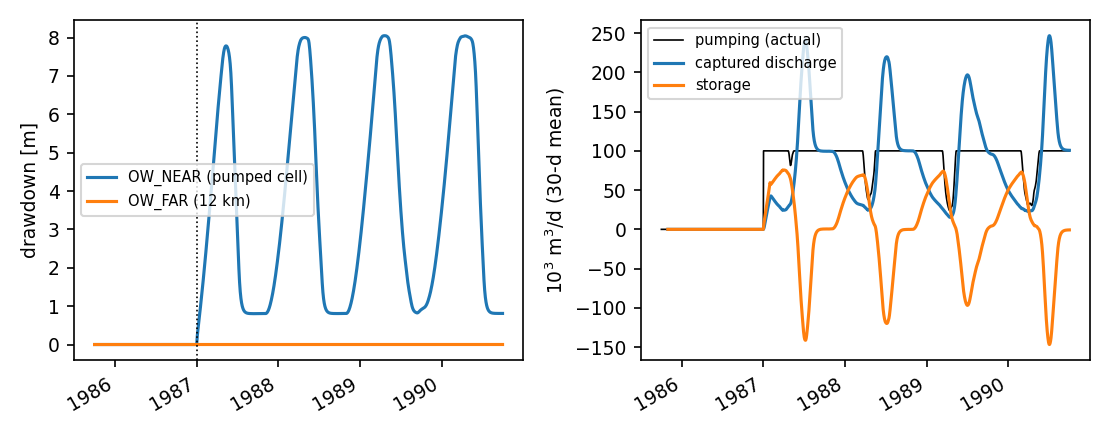
\includegraphics[width=\linewidth]{figures/fig_pumping.png}
\caption{Pumping test: drawdown at the monitoring wells (left) and where the pumped water comes from (right).}\label{fig:upumping}
\end{figure}

\section{The soil zone: CONCEPTUAL or PHYSICAL}\label{sec:usoilzone}
By default (\cmd{:SoilZone CONCEPTUAL}) Raven's soil and the aquifer meet only through recharge and the seepage drain:
Raven's soil never sees the water table.

With \cmd{:SoilZone PHYSICAL} the soil layers you name become the top of the aquifer, owned by Raven. MODFLOW starts below
them. The water table can rise into them: saturated soil drains to the aquifer, recharge stops where the ground is
saturated, and a full soil zone overflows to the surface. This is the arrangement of GSFLOW
\cite{markstrom2008gsflow}.

\begin{plain}
Think of the soil layers you name (for example \cmd{SOIL[0]} and \cmd{SOIL[1]}) as the top of the aquifer, owned by
Raven. MODFLOW starts below them. When the water table climbs to the bottom of the soil, it carries on rising inside the
soil layers; rain falling on that saturated ground cannot soak down any more and stays in the soil, and once the soil is
full the extra water runs off. When it is dry, saturated soil drains down into the aquifer again. On a slope this
happens first at the bottom of the hill, because Raven checks the ground height at many points in each cell.
\end{plain}

\begin{table}[!htbp]\centering
\caption{Which soil-zone option to use.}\label{tab:uszchoice}
\begin{tabularx}{\linewidth}{P{0.25\linewidth}Y}\toprule\hdr
Option & Use it when\\\midrule
\cmd{CONCEPTUAL} (default) & the water table stays below the soil, or for a first model\\
\cmd{PHYSICAL} & the water table reaches the soil: valley floors, wetlands, the foot of slopes, flat lowlands. It takes more computing time per day\\\bottomrule
\end{tabularx}
\end{table}

\subsection{A water table in the soil, on sloping and irregular land}\label{sec:applysz}
On irregular land the water table meets the soil in some parts of a cell and not in others (Figure~\ref{fig:uszsubgrid}).
\begin{figure}[!htbp]\centering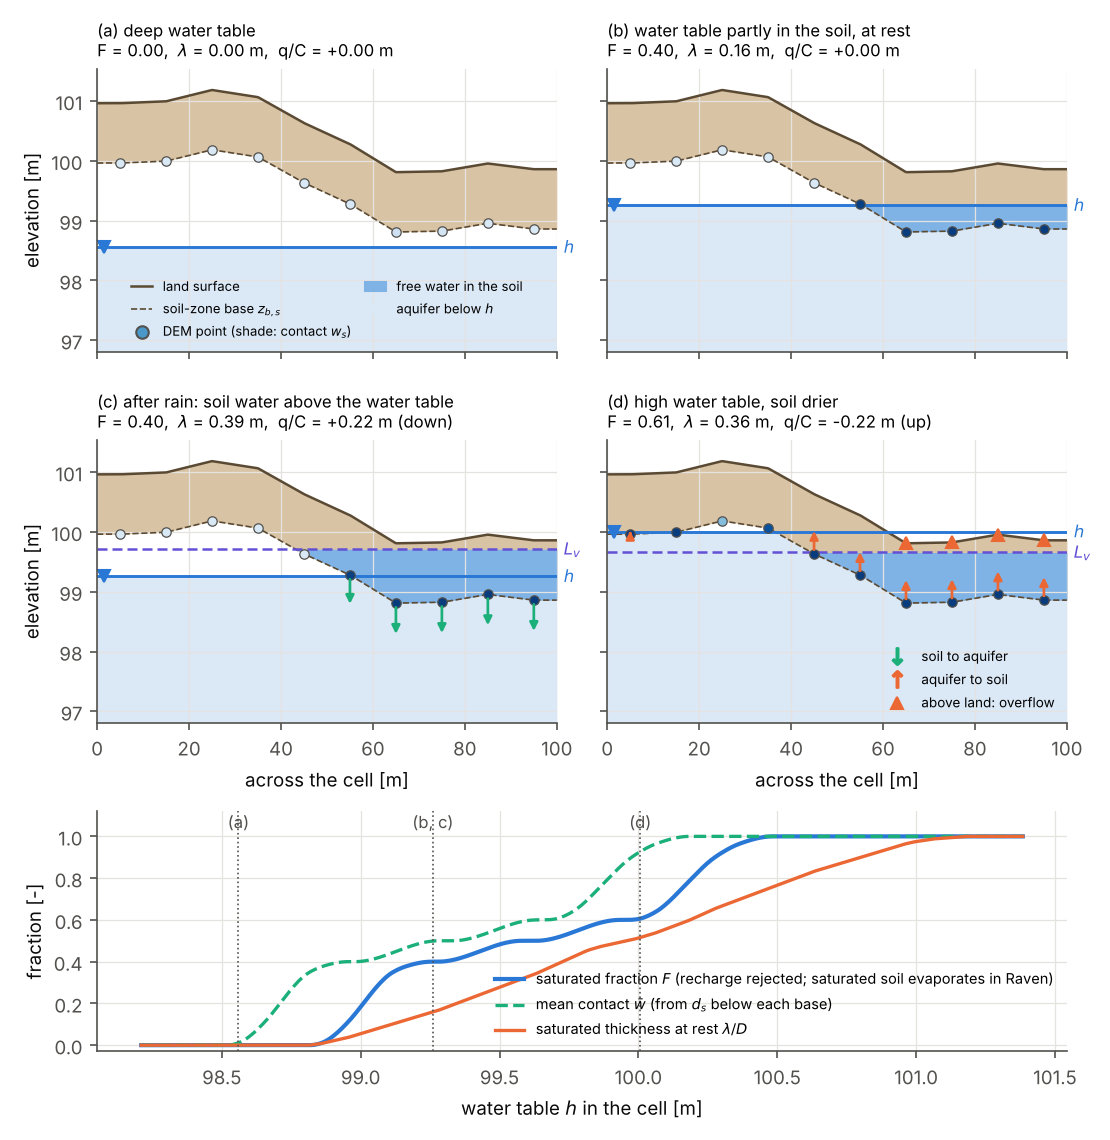
\includegraphics[width=\linewidth]{figures/fig_sz_subgrid.png}
\caption{One 100~m cell with irregular land. Raven samples the land inside each cell at many points (circles). (a) to (d): four positions of the water table and of the water in the soil; the arrows show how much of the exchange between soil and aquifer each point carries, and only the part of the cell where the water table reaches the soil (the saturated fraction) is wet. Bottom: that fraction against the water table.}\label{fig:uszsubgrid}
\end{figure}
Figure~\ref{fig:uszregimes} shows every position the water table can take, and what carries the water in each.
\begin{figure}[!htbp]\centering% Positions of the water table relative to the soil zone and what carries the water in each
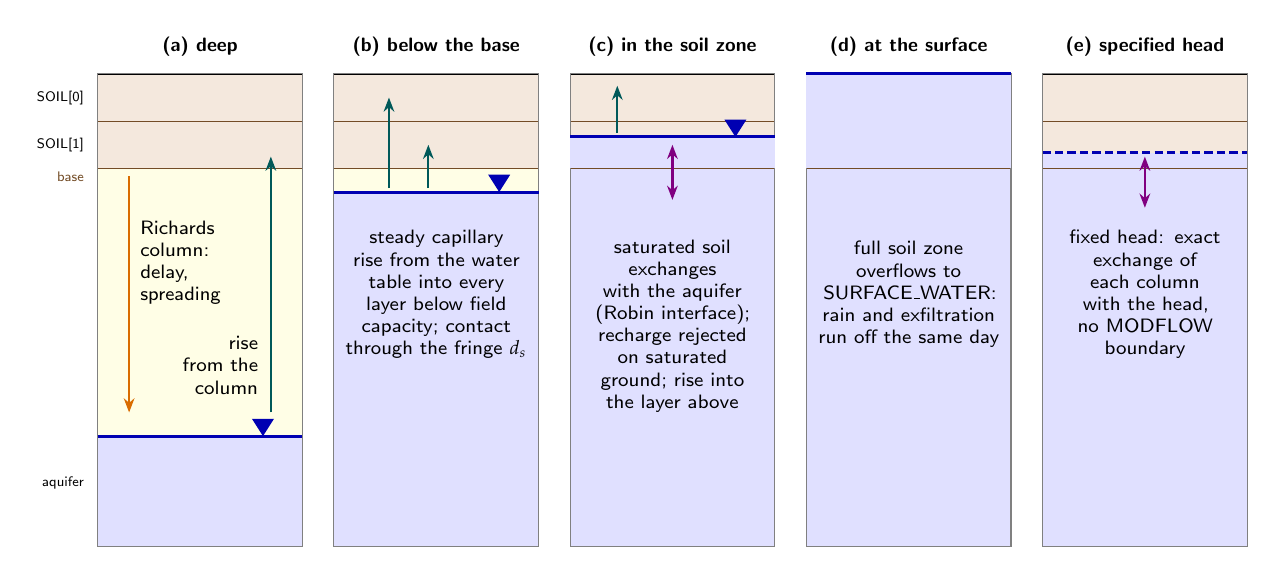
\begin{tikzpicture}[font=\sffamily\scriptsize,x=1mm,y=1mm,
  soil/.style={fill=brown!18,draw=brown!60!black,line width=0.4pt},
  unsat/.style={fill=yellow!10,draw=none},
  sat/.style={fill=blue!12,draw=none},
  wt/.style={blue!70!black,line width=1.1pt},
  base/.style={brown!60!black,dashed,line width=0.6pt},
  up/.style={-{Stealth[length=1.8mm]},line width=0.8pt,teal!70!black},
  dn/.style={-{Stealth[length=1.8mm]},line width=0.8pt,orange!85!black},
  lab/.style={align=center,text width=23mm,inner sep=1pt}]
% one panel: x offset #1, water-table elevation #2 (land 60, soil base 48, soil layers 48-54-60)
\newcommand{\panel}[2]{%
  \fill[sat] (#1,0) rectangle (#1+26,#2);
  \fill[unsat] (#1,#2) rectangle (#1+26,48);
  \draw[soil] (#1,48) rectangle (#1+26,54);
  \draw[soil] (#1,54) rectangle (#1+26,60);
  \draw[base] (#1,48) -- (#1+26,48);
  \draw[line width=0.8pt] (#1,60) -- (#1+26,60);
  \draw[gray] (#1,0) rectangle (#1+26,60);}
% (a) deep water table
\panel{0}{14}
\draw[wt] (0,14) -- (26,14); \fill[blue!70!black] (21,14) -- ++(-1.4,2.2) -- ++(2.8,0) -- cycle;
\draw[dn] (4,47) -- (4,17); \node[lab,text width=13mm,align=left,anchor=west] at (5,36) {Richards column: delay, spreading};
\draw[up] (22,17) -- (22,49.5); \node[lab,text width=12mm,align=right,anchor=east] at (20.8,23) {rise from the column};
% (b) just below the soil base
\panel{30}{45}
\draw[wt] (30,45) -- (56,45); \fill[blue!70!black] (51,45) -- ++(-1.4,2.2) -- ++(2.8,0) -- cycle;
\draw[up] (37,45.5) -- (37,57); \draw[up] (42,45.5) -- (42,51);
\node[lab] at (43,32) {steady capillary rise from the water table into every layer below field capacity; contact through the fringe $d_s$};
% (c) in the soil zone
\panel{60}{52}
\fill[sat] (60,48) rectangle (86,52); \draw[wt] (60,52) -- (86,52); \fill[blue!70!black] (81,52) -- ++(-1.4,2.2) -- ++(2.8,0) -- cycle;
\draw[up] (66,52.5) -- (66,58.5);
\draw[{Stealth[length=1.8mm]}-{Stealth[length=1.8mm]},line width=0.8pt,violet] (73,44) -- (73,51);
\node[lab] at (73,28) {saturated soil exchanges with the aquifer (Robin interface); recharge rejected on saturated ground; rise into the layer above};
% (d) at the land surface
\panel{90}{60}
\fill[sat] (90,48) rectangle (116,60); \draw[wt] (90,60) -- (116,60);
\node[lab] at (103,32) {full soil zone overflows to SURFACE\_\-WATER: rain and exfiltration run off the same day};
% (e) specified head
\panel{120}{50}
\fill[sat] (120,48) rectangle (146,50); \draw[wt,dash pattern=on 3pt off 1.5pt] (120,50) -- (146,50);
\draw[{Stealth[length=1.8mm]}-{Stealth[length=1.8mm]},line width=0.8pt,violet] (133,43) -- (133,49.5);
\node[lab] at (133,32) {fixed head: exact exchange of each column with the head, no MODFLOW boundary};
% labels
\foreach \x/\t in {0/(a) deep,30/(b) below the base,60/(c) in the soil zone,90/(d) at the surface,120/(e) specified head}{
  \node[font=\sffamily\bfseries\scriptsize,anchor=south] at (\x+13,61) {\t};}
\node[anchor=east,font=\sffamily\tiny] at (-0.5,57) {SOIL[0]}; \node[anchor=east,font=\sffamily\tiny] at (-0.5,51) {SOIL[1]};
\node[anchor=east,font=\sffamily\tiny,brown!60!black] at (-0.5,47) {base}; \node[anchor=east,font=\sffamily\tiny] at (-0.5,8) {aquifer};
\end{tikzpicture}

\caption{Where the water table can be and what moves the water in each case. (a) Deep: recharge crosses an unsaturated
column solved with Richards' equation (\cmd{:SoilZoneVadose RICHARDS}), which delays and spreads it; the column also
feeds capillary rise into the soil zone. (b) Within the column's minimum length below the soil base: no column; the
exchange starts through the fringe $d_s$, and capillary rise from the water table reaches the layers above. (c) In the
soil zone: the saturated soil exchanges with the aquifer, recharge on saturated ground is rejected, capillary rise
continues into the layers above the water table. (d) At the surface: the full soil zone overflows. (e) Over a specified
head: each column exchanges with the fixed head exactly.}\label{fig:uszregimes}
\end{figure}
Where the water table comes close to the land --- valley bottoms, the foot of slopes, wetlands, flat lowlands --- add the
soil zone: the water table can then rise into Raven's soil layers, saturated ground rejects recharge, groundwater
discharges into the soil, and full soil overflows to surface water. Nothing else of the model changes.
\begin{enumerate}
\item \textbf{Choose the soil-zone layers} (\cmd{.rvg}): the physical soil layers above the aquifer, usually the top one
or two, \cmd{:SoilZone PHYSICAL SOIL[0] SOIL[1]}. MODFLOW's top then lies one soil-zone thickness below the land, cell by
cell, so the model's top follows the slope.
\item \textbf{Send recharge from the bottom soil-zone layer} (\cmd{.rvi}): for example
\cmd{:Percolation PERC\_GAWSER SOIL[1] GROUNDWATER}, conditional on the coupled HRUs. A drainage that moves only water above
field capacity lets a soil zone that is not connected to the water table pass the rain on.
\item \textbf{Soil parameters} (\cmd{.rvp}): \cmd{POROSITY}, \cmd{FIELD\_CAPACITY} ($<1$), and \cmd{HYDRAUL\_COND} [mm/d] for
the class of the bottom soil-zone layer; \cmd{CLAPP\_B} and \cmd{AIR\_ENTRY\_PRESSURE} for capillary rise. Give the top
aquifer layer a specific yield close to the soil's drainable porosity, $\eta(1-S_{\mathrm{fc}})$ (porosity $\eta$ times
one minus the field capacity $S_{\mathrm{fc}}$): otherwise the water table rises at different rates below and inside the
soil (Raven warns).
\item \textbf{Sloping and irregular land}: give a DEM finer than the cells. Each cell samples it at
\cmd{:SoilZoneSubgrid} $n$ points per side (5 by default, 25 points), so within a cell the low ground saturates first
and the high ground later (Reference, Figure~\ref{R-fig:szsubgrid}; Figure~\ref{fig:uszhillslope} shows a coupled hillslope). Between cells MODFLOW's heads carry the water down
the slope, and the saturated area spreads up from the foot of the slope and from hollows and retreats downslope as it
dries (Reference, Figure~\ref{R-fig:szhillslope}). Keep \cmd{SEEPAGE\_SMOOTHING\_DEPTH} (the contact depth $d_s$) at
0.1--0.5~m. Seepage faces and saturated strips narrower than a cell need smaller cells (or \cmd{:GridRefinement} along
valleys); within a cell the soil water stands at one level.
\begin{figure}[!htbp]\centering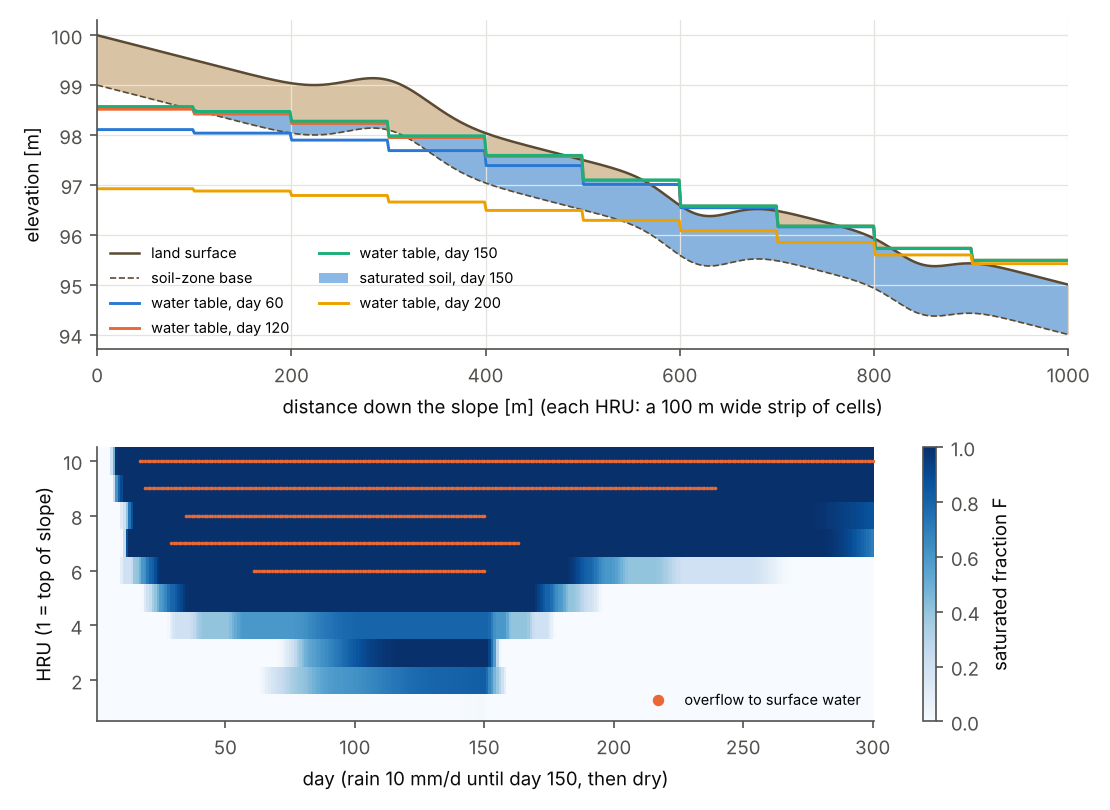
\includegraphics[width=\linewidth]{figures/fig_sz_hillslope.png}
\caption{Coupled hillslope with irregular land (rain 10~mm/d for 150 days, then dry). Top: land surface, soil-zone base and
the water table of each cell on four days; shaded, the saturated soil on day 150. Bottom: saturated fraction $F$ of each
HRU over time (1 = top of the slope), with the days on which the HRU overflows to surface water.}\label{fig:uszhillslope}
\end{figure}
\item \textbf{A deep water table elsewhere}: \cmd{:SoilZoneVadose RICHARDS} (or \cmd{KINEMATIC}, \cmd{LAG}) carries the
recharge through the unsaturated zone between the soil and the water table, with its delay (Section~\ref{sec:uvadose}).
On hummocky ground \cmd{:SoilZoneVadoseClasses} 3 gives the hollows and the hummocks their own columns (Reference,
Section~\ref{R-sec:vzclasses}). Capillary rise from a shallow water table is then on by default. Reference,
Figure~\ref{R-fig:szregimes}, shows every position of the water table and what carries the water in each; the coupling
moves between them without any setting.
\item \textbf{HRUs that are wet at the foot and dry at the top}: \cmd{:SoilZoneClasses} 3--5 runs Raven's processes on
classes of an HRU's columns (needs \cmd{:Method ORDERED\_SERIES}).
\item \textbf{Check}: \cmd{GWSoilExchange.csv} gives, per HRU and step, the soil-zone base, the soil water level, the water
table and the saturated fraction $F$; \cmd{tools/plot\_soilzone.py} plots them, and \cmd{tools\_audit.py} closes every
soil-zone identity. The interface should converge on every step (\cmd{GWBudget.csv}, \emph{interface converged}).
\end{enumerate}
The coupling has been checked on planar and irregular hillslopes against a MODFLOW-only reference (Reference,
Section~\ref{R-sec:vszbasic}) and on 400 randomly drawn rough-terrain cases (1\,620 runs with the four unsaturated-zone
methods and the regression cases) with slopes up to 30\,\%, pits, cliffs, ridges, sloping and pinching layers and DEMs
coarser or finer than the grid (Reference, Section~\ref{R-sec:vrough}). The reference for every command is Reference,
Table~\ref{R-tab:szcmds}. Workshop~3 takes you through these steps.

\subsection{The unsaturated zone: NONE, RICHARDS, KINEMATIC or LAG}\label{sec:uvadose}
When the water table lies well below the soil, rain that drains out of the soil takes days to weeks to reach it, and
arrives spread out. \cmd{:SoilZoneVadose} chooses how that trip through the dry ground is computed. It applies only with
\cmd{:SoilZone PHYSICAL}.
\begin{table}[!htbp]\centering
\caption{The four methods of \cmd{:SoilZoneVadose}.}\label{tab:uvadose}
\begin{tabularx}{\linewidth}{P{0.17\linewidth}P{0.37\linewidth}Y}\toprule\hdr
Method & What it does & Use it when\\\midrule
\cmd{NONE} (default) & recharge reaches the water table in the step & the water table is shallow, or the timing of recharge does not matter\\
\cmd{RICHARDS} & Richards' equation on a column of nodes, from the soil's retention curve; capillary rise also from the column & the reference method: the timing matters and the materials are known\\
\cmd{KINEMATIC} & Richards' equation without capillary forces (as MODFLOW's UZF package and GSFLOW) & a delay that depends on the flux, at a fraction of the cost; it cannot fail to converge\\
\cmd{LAG} & a cascade of linear stores with a travel time per metre $t_m$ & only the delay and spreading matter; $t_m$ is the one parameter to calibrate (0: derived from each material)\\\bottomrule
\end{tabularx}
\end{table}
\begin{whattowrite}
\cmd{:SoilZoneVadose RICHARDS}\quad or\quad \cmd{:SoilZoneVadose KINEMATIC}\quad or\quad \cmd{:SoilZoneVadose LAG 2}\\
\cmd{:SoilZoneVadoseClasses 3}\quad (optional: hollows and hummocks get their own columns)
\end{whattowrite}
The columns use \cmd{POROSITY}, \cmd{CLAPP\_B} and \cmd{AIR\_ENTRY\_PRESSURE} of the aquifer classes (defaults 0.3, 4
and 0.3~m; for an existing model, those of \cmd{:SoilZoneAquiferClass}).

\begin{example}[: a storm over a deep water table]
A 3-day storm of 40~mm/d on soil over a water table 6~m deep, in sand (test P1 of the Reference). Without a column the
recharge reaches MODFLOW with the percolation, centred on day~6.1. With \cmd{RICHARDS} it arrives spread over two weeks,
its peak 45\% lower, centred on day~15.6. With \cmd{LAG 2} the centre is on day~13.9, with \cmd{LAG 4} on day~21.1.
Nothing is lost in any of them.
\end{example}

Figures~\ref{fig:uvzkinematic} and \ref{fig:uvzlag} show how \cmd{KINEMATIC} and \cmd{LAG} delay and spread the
recharge, and Figure~\ref{fig:uvzclasses} how \cmd{:SoilZoneVadoseClasses} groups the low and high parts of a cell.
\begin{figure}[!htbp]\centering
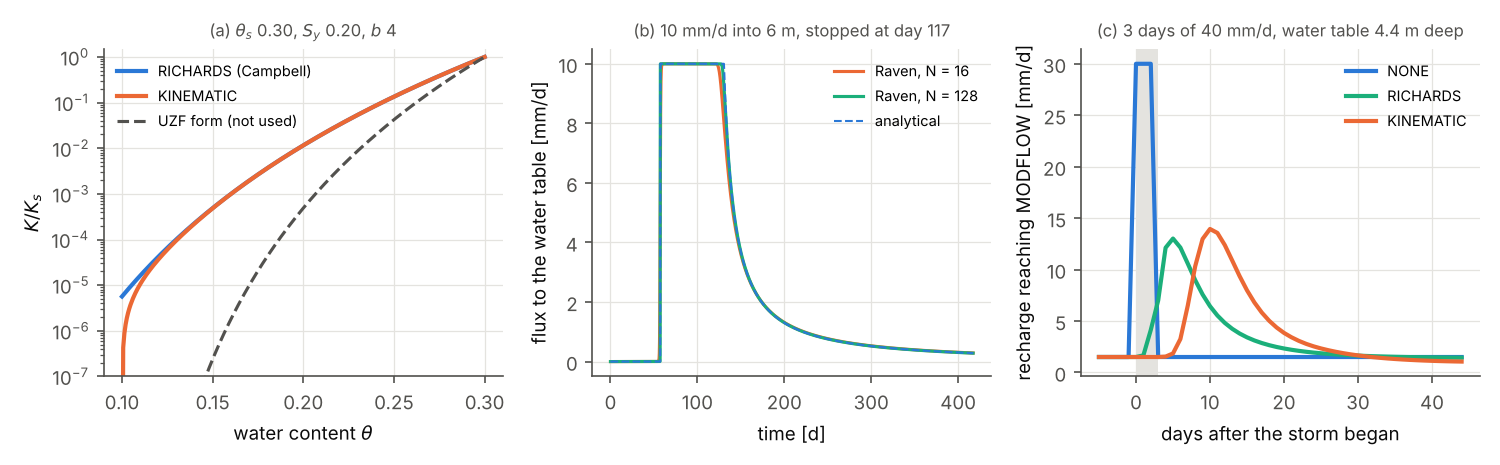
\includegraphics[width=\textwidth]{figures/fig_vz_kinematic.png}
\caption{\cmd{KINEMATIC}. (a) How the ground's conductivity grows as it gets wetter, compared with the curve \cmd{RICHARDS} uses. (b) Rain of 10~mm/d for 117 days over a water table 6~m down: the water reaching the water table, against the exact solution. (c) A 3-day storm over a deep water table: the recharge arrives later and spread out.}\label{fig:uvzkinematic}
\end{figure}
\begin{figure}[!htbp]\centering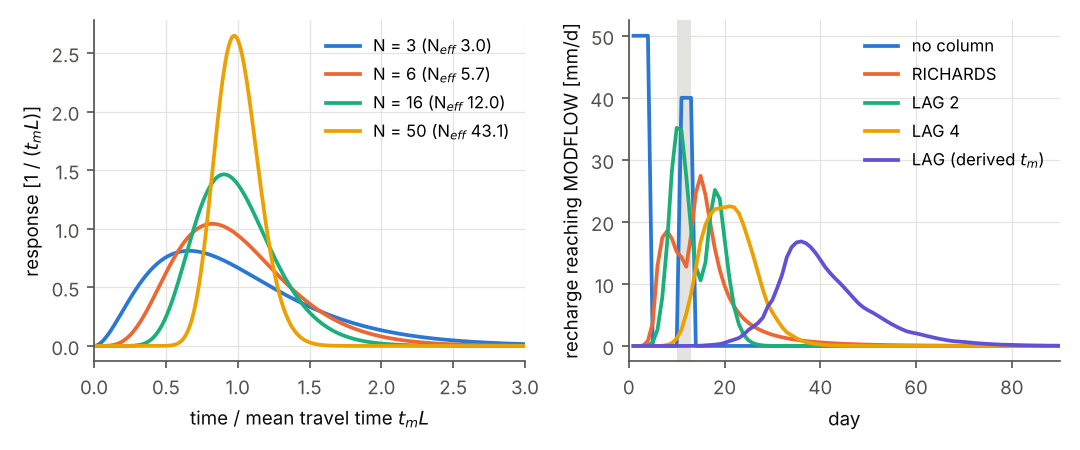
\includegraphics[width=\linewidth]{figures/fig_vz_lag_cascade.png}
\caption{\cmd{LAG}. Left: water entering the top of a column comes out at the bottom spread over time; more nodes give a sharper peak. Right: the recharge from a 3-day storm reaching a water table 6~m down, without a column, with \cmd{RICHARDS} and with \cmd{LAG}.}\label{fig:uvzlag}
\end{figure}
\begin{figure}[!htbp]\centering
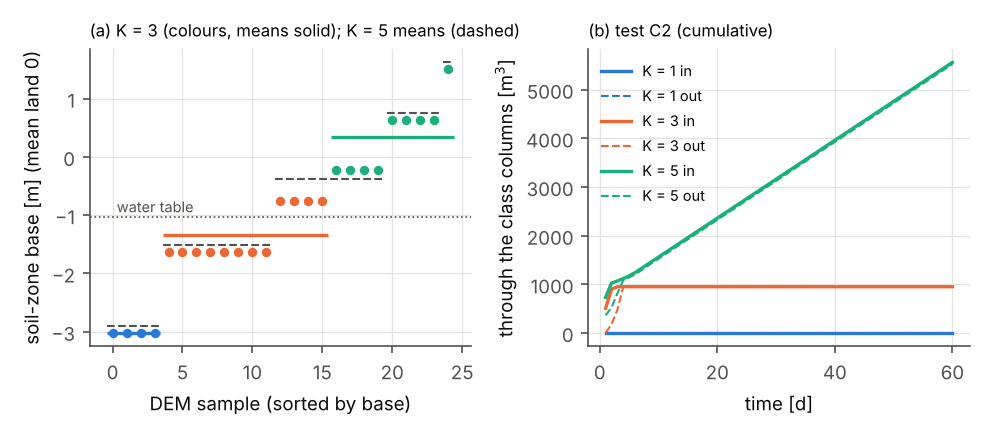
\includegraphics[width=\linewidth]{figures/fig_vz_classes.png}
\caption{Depth classes. (a) The 25 sample points of a hummocky cell, sorted by depth and grouped into 3 classes (colours) or 5; each class gets its own column. (b) The water entering and leaving the class columns in a test, summed over time.}\label{fig:uvzclasses}
\end{figure}
\paragraph{Capillary rise.} When the water table is shallow, dry soil also pulls water up from it, so plants and
evaporation keep drawing on groundwater after the rain stops. \cmd{:SoilZoneCapillaryRise} is \cmd{ON} by default with
\cmd{RICHARDS}, \cmd{KINEMATIC} and \cmd{LAG}, and \cmd{OFF} with \cmd{NONE}. It is computed from the soil's own retention
curve, not from a fitted rate.

\paragraph{Cost.} On the Liard example with \cmd{:SoilZone PHYSICAL} (85 HRUs, one year) the run takes 69~s with the
defaults, and 91~s with unsaturated columns, capillary rise and three classes. MODFLOW's solve remains the larger part.

\section{Common questions}
\paragraph{Can only part of my watershed have groundwater?} Yes. Only HRUs with an \cmd{AQUIFER\_PROFILE} are coupled; all
others run exactly as they do without groundwater.
\paragraph{Can two aquifer systems exchange water?} Yes, when their cells touch: lateral flow between neighbouring profiles
and leakage between layers are computed by MODFLOW like any other flow.
\paragraph{What happens where the water table reaches the surface?} The seepage drains return the water to Raven, where it
follows Raven's processes (for example baseflow to the river).
\paragraph{Can the aquifer take more water than a river carries?} Not from a river Raven builds: the supply limit caps
each river cell's largest possible loss at its share of the reach's flow at the start of the step, and the loss is taken
from the reach's runoff, inflow and outflow, so the outflow leaving the watershed falls by it. Only a reach whose flow stops
within the step can leave part of its loss to be carried to the next step (warned about; the loss carried at the end of
the run is a run total of \cmd{GWModelSummary.txt}). An existing model's stream package keeps its own conductance and has
no supply limit (Reference, Section~\ref{R-sec:extlimits}): a losing reach can take more than the channel holds, and the
part the channel cannot supply is carried to the next step (\emph{river loss carried to next step}; exactly accounted).
Example~B does this for months: the carry reaches about $10^{8}$~m$^3$ and is repaid by the end of the run.
\paragraph{Does frozen ground limit recharge?} Recharge is whatever Raven's processes send to \cmd{GROUNDWATER}, so frozen
ground acts on it through Raven's own process choices (a \cmd{:FrozenGround} process, infiltration and percolation methods
that respond to frozen soil); the coupling adds no frozen-ground control of its own.
\paragraph{Does the coupling change results for my other subbasins?} Only through the rivers: groundwater discharge or
losses in coupled subbasins change the flow passed downstream.

\chapter{Running, outputs and the water balance}\label{uch:outputs}
This chapter says how to run a coupled model, what Raven writes, and how to check that the water balance of a run is
right. Reference, Section~\ref{R-ch:outputs}, lists every output column, and Reference, Chapter~\ref{R-ch:c5}, the
accounts behind them.

\section{Running}
A coupled model runs like any Raven model:
\begin{lstlisting}
Raven Liard -o output/
\end{lstlisting}
Raven reads all input files, builds (or copies) the MODFLOW~6 model in \cmd{output/mf6/}, and then runs both models one
time step at a time. A successful run ends with \cmd{Exiting Gracefully: Successful Simulation}. Errors and warnings
are in \cmd{output/Raven\_errors.txt}.

Raven finds the MODFLOW~6 library by itself when it lies next to the Raven program or in \cmd{lib/mf6/} of the Raven
checkout. Otherwise name it with \cmd{:MF6Library path} in the \cmd{.rvg} file, or with the environment variable
\cmd{RAVEN\_MF6\_LIB}.

\section{The output files}
All rows are stamped with the date at the \emph{end} of the step, the moment the values refer to.
\begin{table}[!htbp]\centering
\caption{The groundwater outputs, beside Raven's usual files.}\label{tab:uoutputs}
\begin{tabularx}{\linewidth}{P{0.27\linewidth}Y}\toprule\hdr
File & What it holds\\\midrule
\cmd{GWModelSummary.txt} & the grid built (layers, cells, active cells, river cells), the MODFLOW library and its version, how each HRU is linked, run totals\\
\cmd{GWBudget.csv} & every step: recharge from Raven, seepage back to Raven, river exchange, storage change, MODFLOW's balance error, and every other exchange\\
\cmd{GWHRUState.csv} & every step: the water table and the depth to water under each coupled HRU\\
\cmd{GWHeads.csv} & the head at each monitoring well ($-1.2345$ when the screened cell is dry)\\
\cmd{GWConnectivity.csv} & the number of separate wet areas of the aquifer, and the wet share of each profile\\
\cmd{GWSoilExchange.csv} & with \cmd{:SoilZone PHYSICAL}: the soil zone of each HRU, every step\\
\cmd{GWHeads.nc} & with \cmd{:WriteNetCDFHeads}: the head in every cell (Raven built with NetCDF)\\
\cmd{Hydrographs.csv}, \cmd{Diagnostics.csv} & streamflow and fit statistics, as in any Raven run; \cmd{Diagnostics.csv} also scores the heads (\cmd{GW\_HEAD})\\
\cmd{WatershedStorage.csv} & Raven's balance; it includes all exchanged water\\
\cmd{solution.rvc} & the end state, with the groundwater blocks, for a restart (Chapter~\ref{uch:restarts})\\
\cmd{mf6/} & the MODFLOW~6 model Raven wrote or copied, its list files and the heads \cmd{gwf.hds}; it can be opened in ModelMuse or FloPy\\
\cmd{mf6/grid\_cells.geojson} & every cell as a longitude/latitude polygon, ready to be joined with heads in QGIS\\\bottomrule
\end{tabularx}
\end{table}

\section{Reading GWModelSummary.txt}
Read it after the first run of a new model. Check that:
\begin{itemize}
\item the grid and the number of active cells are what you expect;
\item every coupled HRU is linked, and its linked share is close to 1;
\item the polygon area of each HRU is close to its \cmd{.rvh} area;
\item with an existing model, the units, the packages taken over and kept, and the HRU coverage are right
(Chapter~\ref{uch:existing}).
\end{itemize}

\section{Reading GWBudget.csv}
\cmd{GWBudget.csv} has one row per step. Its columns are the aquifer's water account for that step, in m$^3$/d:
recharge in, seepage and river discharge out, river leakage in, and so on. \emph{Storage release} closes the account:
water released from the aquifer (negative: water stored).
\begin{table}[!htbp]\centering
\caption{The main columns of \cmd{GWBudget.csv}. Reference, Section~\ref{R-app:outputs}, lists them all.}\label{tab:ubudget}
\begin{tabularx}{\linewidth}{P{0.4\linewidth}Y}\toprule\hdr
Column & Meaning\\\midrule
time, date & model time [d] and date at the end of the step\\
Raven recharge, MF6 recharge & recharge leaving Raven, and entering MODFLOW\\
seepage to Raven, returned to Raven & drain discharge at the model top, and the volume added to Raven's stores\\
river leakage to aquifer, aquifer discharge to rivers & the river exchange, each direction\\
river loss carried to next step & a river loss the reach could not supply in the step (normally 0)\\
storage release & water released from aquifer storage (negative: stored)\\
MF6 balance error [m$^3$/d], [\%] & MODFLOW's balance error, and relative to the gross flow\\
outer iterations, converged & iterations used; 1 converged, 2 accepted at the relaxed tolerance, 0 not converged\\
water-table ET; wells specified, actual; GHB, CHD & the other exchanges (boundaries positive into the aquifer)\\
other model packages & with an existing model: net flow of the model's own packages\\
soil zone to aquifer, aquifer to soil zone, \dots & with \cmd{:SoilZone PHYSICAL}: the soil-zone exchange and its interface\\\bottomrule
\end{tabularx}
\end{table}

\begin{example}[: 15 June 1996 in the Liard run]
Recharge from Raven 21.4 million m$^3$/d and river leakage 3.0 million flowed in; seepage to Raven 19.1 million and
discharge to rivers 1.3 million flowed out. The aquifer stored the difference, 3.9 million m$^3$ (storage release
$-3\,925\,212$~m$^3$/d): a water-table rise of about 1~mm on average. Inflows minus outflows plus release is
0.00003~m$^3$/d, a relative error of about $10^{-10}$. Reference, Section~\ref{R-ch:balance}, shows Raven's side of the
same day.
\end{example}

\subsection{What a good run looks like}
\begin{enumerate}
\item \emph{MF6 balance error [\%]} stays well below 0.1\% every step. Larger values point to a step that did not
converge, or a head tolerance that is too loose (\cmd{:SolverHead\allowbreak Tolerance}, default 0.00001~m).
\item \emph{Raven recharge} and \emph{MF6 recharge} are equal, unless a recharge delay or fixed-head cells are used, or
recharge is rejected on saturated ground (\cmd{:SoilZone PHYSICAL}).
\item \emph{returned to Raven} equals \emph{seepage to Raven}.
\item \emph{converged} is 1 on every step (2: accepted at a relaxed tolerance; 0: not converged). Steps that did not
converge are flagged; see Chapter~\ref{uch:trouble}.
\item \emph{river loss carried to next step} is 0, except for a reach whose flow stopped within the step, a reservoir gain
MODFLOW did not supply (taken from the reach), or an existing model's stream package (Chapter~\ref{uch:existing}). The
carry is taken from the river the next step, and Raven warns.
\item With \cmd{:SoilZone PHYSICAL}: \emph{soil-zone shortfall} is zero and \emph{interface converged} is 1 on (nearly)
every step.
\item Raven's \cmd{WatershedStorage.csv} balance error stays at the first step's value (Raven's own, the same without
groundwater), apart from Raven's own known errors (Reference, Section~\ref{R-ch:limits}).
\end{enumerate}
Reference, Section~\ref{R-ch:balance}, gives the rules behind each item.

\section{The audit tool}\label{sec:uaudit}
\cmd{tools\_audit.py} checks all of these automatically. It lies in \cmd{examples/Liard\_groundwater/} and needs Python~3
with pandas:
\begin{lstlisting}
python tools_audit.py output
python ../Liard_groundwater/tools_audit.py output      # from example B's folder
\end{lstlisting}
Lines to look at:
\begin{itemize}
\item \cmd{recharge: (Raven - MF6 - dStore - toCHD)/Raven} should be 0;
\item \cmd{MF6 cumulative residual / gross flow} about $10^{-10}$ or smaller;
\item \cmd{unconverged steps} 0;
\item \cmd{ERROR lines} 0.
\end{itemize}
For example~B, a test run gave: recharge identity 0, \cmd{MF6 cumulative residual / gross flow} about $-1.9\times10^{-11}$,
\cmd{unconverged steps} 0, river bookkeeping about $-5\times10^{-12}$, \cmd{ERROR lines} 0 and \cmd{max outer iterations}
245 (the first step). With \cmd{:SoilZone PHYSICAL} the tool also closes every soil-zone identity.

\section{Heads everywhere, and particle tracking}
\begin{itemize}
\item \cmd{mf6/gwf.hds} (MODFLOW binary, readable with FloPy) holds the head in every cell every \cmd{:HeadSaveFrequency}
steps (default 30). \cmd{GWHeads.nc} holds them with \cmd{:WriteNetCDFHeads}.
\item With \cmd{:WriteGWBudgetFile} a generated model also saves MODFLOW's cell-by-cell flows (\cmd{mf6/gwf.cbc}) and the
porosity (\cmd{mf6/gwf.porosity}). \cmd{tools/make\_prt.py} then builds and runs a MODFLOW~6 particle-tracking model (PRT)
on the coupled flows, forward or backward from the wells (capture zones, travel times). PRT needs \cmd{:HeadSaveFrequency 1}.
Reference, Section~\ref{R-sec:budgetfile}, and Workshop~5 give the details.
\end{itemize}

\chapter{Restarts, ensembles and calibration}\label{uch:restarts}
This chapter covers what you do with a working model: start it well, split or continue long runs, run ensembles and
calibrate. Workshop~5 practises restarts, ensembles and particle tracking; Workshop~6 calibration with Ostrich.

\section{Spin-up}
\paragraph{How long a spin-up do I need?} Start from a steady state with the long-term mean recharge
(\cmd{:GWInitialization STEADY\_STATE r}, Section~\ref{sec:ustart}). Then check that \emph{storage release} in
\cmd{GWBudget.csv} averages near zero over the first years. Large, slow aquifers may need decades.

\section{Restarts (hotstart)}\label{sec:urestart}
At the end of a run Raven writes \cmd{solution.rvc}. Besides Raven's own states it holds the groundwater blocks: the head
in every cell (\cmd{:GWHeads}) and, when they are used, the recharge delay stores, the river loss carried, the reservoir
seepage in transit, and the soil-zone and unsaturated columns.
\begin{whattowrite}
Use \cmd{solution.rvc} of the finished run as the \cmd{.rvc} file of the next run, and set \cmd{:StartDate} in its
\cmd{.rvi} to the end of the first run.
\end{whattowrite}
A coupled run continued this way carries on exactly: every value of the file is written with 17 significant digits, so the
restarted run starts from the states the continuous run had, bit for bit. A run without groundwater continues from
Raven's usual 5-decimal states. The blocks are read back automatically; a damaged value stops the run with a message
naming the block.

The steady-state start of \cmd{:GWInitialization} is skipped on a restart. For an existing MODFLOW model, see
Section~\ref{sec:uextrestart}: a restart carries only the heads, and some packages cannot be restarted. Reference,
Section~\ref{R-sec:hotstart}, gives every block and rule.

\section{Ensembles}
Raven's ensemble modes (Monte Carlo, DDS, EnKF) run the model several times in one program run. For every member the
groundwater model is rebuilt from scratch, MODFLOW is restarted, and its files go to that member's output folder. Each
member starts with a fresh water balance and, unless its own \cmd{.rvc} says otherwise, from the state of the first run.
An EnKF member's own time series file may give its own well rates and boundary heads. Reference, Chapter~\ref{R-ch:c5},
gives the rules.

\section{Calibration}\label{ch:calib}
Aquifer class and profile parameters are ordinary entries in the \cmd{.rvp} file, so they can be calibrated with Ostrich
exactly like soil parameters: make a template of the \cmd{.rvp} with parameter names in place of values.
\par\noindent\begin{minipage}{\linewidth}
\begin{lstlisting}
  GRAVEL,      par_K_gravel, 5.0,  1.0E-5, par_Sy_gravel, 0.30
  UPLAND_TILL, par_K_till,   0.02, 1.0E-4, 0.08,          0.30
\end{lstlisting}
\end{minipage}\par\smallskip
\begin{itemize}
\item Monitoring-well heads (\cmd{:ObservationData GW\_HEAD}) are scored in \cmd{Diagnostics.csv} next to streamflow, so an
objective can combine both.
\item Calibrate conductivities on a logarithmic scale.
\item \cmd{docs/ostrich\_example/} contains an \cmd{ostIn.txt} using DDS \cite{tolson2007dds}, the template and run scripts.
\item Because the linkage is cached, repeated runs skip the geometry work.
\item The coupling works in an ensemble and with Ostrich: each ensemble member rebuilds and restarts MODFLOW.
\end{itemize}

\subsection{A synthetic test}
Groundwater under subbasin 52 only (545 active columns), 2 years, 7 s per run. Heads from a run with known parameters, plus
2 cm of random noise, at four monitoring wells were the observations. The search started from values 2.5 to 10 times off.
\begin{table}[!htbp]\centering
\caption{Synthetic calibration: the parameters that made the ``observations'', the starting values, and the values DDS recovered (the error is that of the value shown against the true value).}\label{tab:synthcal}
\begin{tabular}{lrrrr}\toprule\hdr
Parameter & True & Start & After 150 runs & Error\\\midrule
Gravel $K$ [m/d] & 50 & 5 & 47.7 & $-4.6$\%\\
Gravel $S_y$ & 0.25 & 0.10 & 0.239 & $-4.4$\%\\
Upland-till $K$ [m/d] & 0.2 & 2.0 & 0.149 & $-25.5$\%\\\bottomrule
\end{tabular}\end{table}
Table~\ref{tab:synthcal} shows the result. The objective (the sum of RMSE over the four wells) fell from 14.4 m to 0.17 m.
It is 0.08 m at the true values, so more runs would refine it further (Figure~\ref{fig:calib}). The upland-till
conductivity is the hardest to identify, because the upland heads respond weakly to it.
\begin{figure}[!htbp]\centering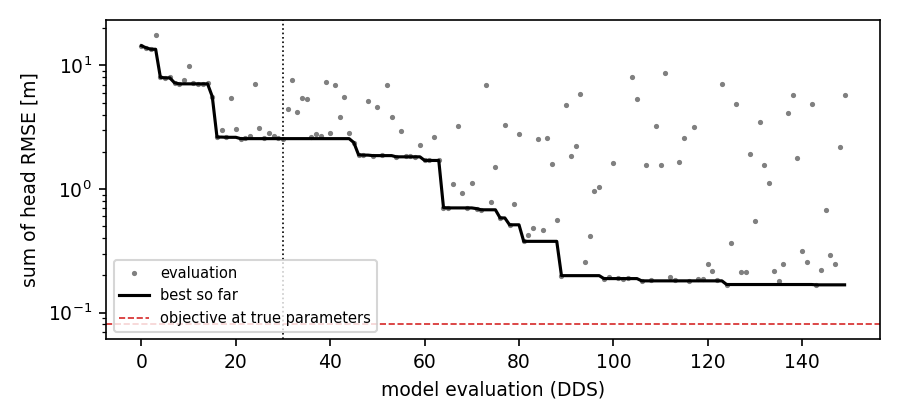
\includegraphics[width=0.8\linewidth]{figures/fig_calibration.png}
\caption{Synthetic calibration: objective against model runs.}\label{fig:calib}\end{figure}

\subsection{The Ostrich input file, line by line}
\begin{lstlisting}
ProgramType         DDS             # search algorithm (dynamically dimensioned search)
ObjectiveFunction   GCOP            # general constrained optimization
ModelExecutable     ./Ost-Raven.sh  # script that runs Raven in ./model
BeginFilePairs
  Liard.rvp.tpl ; model/Liard.rvp   # template -> model file with values filled in
EndFilePairs
BeginParams                         # name, start, lower, upper, transformations
  par_K_gravel   5.0  1.0  500.0  none log10 none
  par_Sy_gravel  0.10 0.05 0.35   none none  none
  par_K_till     2.0  0.01 5.0    none log10 none
EndParams
BeginResponseVars                   # values read from Diagnostics.csv
  RMSE1  model/output/Diagnostics.csv ; OST_NULL 1 4 ','  # line 1 (header = 0), column 4
  ...
EndResponseVars
BeginTiedRespVars                   # objective = sum of the RMSEs
  SUM_RMSE 4 RMSE1 RMSE2 RMSE3 RMSE4 wsum 1.0 1.0 1.0 1.0
EndTiedRespVars
BeginGCOP
  CostFunction SUM_RMSE
EndGCOP
BeginDDSAlg
  MaxIterations 150
EndDDSAlg
\end{lstlisting}
Ostrich counts the lines of \cmd{Diagnostics.csv} from 0 (the header is line 0) and its columns from 1. With
\cmd{:EvaluationMetrics NASH\_SUTCLIFFE RMSE KLING\_GUPTA} the columns are the series, the file, NSE, RMSE (column 4) and
KGE. The four \cmd{GW\_HEAD} series are lines 1--4 when they are the model's only observations. With four monitoring wells
added to the Liard example, whose 29 streamflow series come first, they are lines 30--33. Check the line and column of
each response in your own \cmd{Diagnostics.csv}: they depend on the order of observations and on
\cmd{:EvaluationMetrics}. To combine heads and streamflow, add NSE or KGE responses of the hydrographs with suitable
weights.

\chapter{Troubleshooting}\label{uch:trouble}
Raven checks the inputs at start-up and stops with a message that names the problem, in \cmd{Raven\_errors.txt}. This
chapter covers the most common messages and symptoms. Reference, Sections~\ref{R-app:errors} and~\ref{R-app:warnings},
list every message.

\section{Messages and symptoms}\label{ch:trouble}
\begin{longtable}{P{0.36\linewidth}P{0.588\linewidth}}
\caption{Messages and symptoms, with their causes and remedies.}\label{tab:utrouble}\\
\toprule\hdr
Message or symptom & Cause and remedy\\\midrule\endfirsthead
\caption[]{Messages and symptoms, with their causes and remedies (continued).}\\
\toprule\hdr
Message or symptom & Cause and remedy\\\midrule\endhead
``cannot load MODFLOW 6 library'' & run \cmd{python tools/get\_mf6.py} of RavenHydroFramework-extra, or set \cmd{:MF6Library} or \cmd{RAVEN\_MF6\_LIB} to the full path of \cmd{libmf6}; the message lists the places searched\\
``the MODFLOW 6 library \dots\ is version \dots; the coupling needs MODFLOW 6 6.5.0 or newer'' & an old library was found first: remove the \cmd{:MF6Library} or \cmd{RAVEN\_MF6\_LIB} naming it, and get 6.8.1 (Section~\ref{sec:uinstall})\\
``MODFLOW 6 stopped the run during \dots'' & MODFLOW found an input error inside its library; the message (also in \cmd{Raven\_errors.txt}) quotes the error report of \cmd{<output>/mf6/mfsim.lst}\\
``Cannot find file'' & run Raven from inside the model's folder; example~B also needs \cmd{../Liard\_groundwater}\\
``GeoJSON file \dots\ is in EPSG:\emph{n}'' / ``\dots\ outside the longitude/latitude range'' & a projected input file: give \cmd{:InputCRS} (Section~\ref{sec:uinputcrs})\\
a raster's band unit is not metres & convert the values, or write \cmd{METRES} after the file name when they are metres (Section~\ref{sec:umetres})\\
``layer \dots\ starts dry'' (warning) & the initial heads leave a whole layer dry; start from \cmd{:GWInitialization STEADY\_STATE}, a smaller \cmd{INITIAL\_HEAD\_DEPTH} or \cmd{:InitialGWHeads}\\
``HRU \dots\ has an AQUIFER\_PROFILE but no polygon'' & HRU IDs in the GeoJSON do not match the \cmd{.rvh}; check the ID field name. When a reason is given (the polygon has no area), fix the HRU's outline\\
``HRU \dots\ references unknown AQUIFER\_PROFILE'' & define the profile in the \cmd{.rvp}\\
``does not overlap any active groundwater cell'' & the HRU is too small for the grid or sits where bedrock is at the surface; reduce \cmd{:GridCellSize} or \cmd{:MinCellCoverage}, or check the bedrock map\\
``polygon area \dots\ differs from .rvh AREA'' & information only; volumes are always consistent\\
``no process moves water into GROUNDWATER'' & route recharge to \cmd{GROUNDWATER} (Step~3 of Chapter~\ref{uch:quick})\\
``process \dots\ removes water from GROUNDWATER'' & a Raven process drains \cmd{GROUNDWATER} in a coupled HRU; restrict it with \cmd{:-->Conditional}\\
``process \dots\ sends water to GROUNDWATER in HRU \dots\ which has no AQUIFER\_PROFILE'' & that water would leave the model; restrict the process\\
``MODFLOW 6 did not converge'' & start from a steady state or realistic heads; raise \cmd{:SolverMax\allowbreak OuterIterations}; increase \cmd{SEEPAGE\_SMOOTHING\_DEPTH}; check for extreme parameter contrasts\\
Well rate is zero (``no :WellFlowRate time series'') & the \cmd{:WellFlowRate} block is missing, or its ID does not match an ID in \cmd{:Wells}\\
``well \dots\ is outside the active groundwater model'' & move the well or enlarge the coupled area\\
``reservoir \dots\ has no :SeepageParameters'' / ``no coupled lake HRU'' & add \cmd{:SeepageParameters}; give the lake HRU an \cmd{AQUIFER\_PROFILE}\\
``running more time steps than the MODFLOW 6 simulation holds'' & \cmd{:Duration} or \cmd{:TimeStep} is inconsistent; rerun\\
existing model: a recharge, ET or UZF package not declared & name it in \cmd{:RavenTakesOver} or \cmd{:KeepPackages} (Chapter~\ref{uch:existing})\\
Water table far above the land surface & \cmd{SEEPAGE\_LEAKANCE} too small, or $K$ too low for the recharge\\
Aquifer steadily emptying for years & initial heads too high; use a steady-state start or a longer spin-up\\\bottomrule
\end{longtable}

\section{Steps that do not converge}
MODFLOW solves each step by repeated improvement (Newton's method). A step has converged when the heads stop changing
within the head tolerance. When a step needs many iterations, Raven relaxes the tolerance for the rest of that step. A
step that still does not converge is flagged in \cmd{GWBudget.csv} (\emph{converged} 0) and the run goes on; the
exchange on that step is limited. The audit tool counts them (\emph{unconverged steps}); the table above gives the
remedies. Reference, Section~\ref{R-ch:mf6}, explains how MODFLOW solves each step.

\section{Frequently asked questions}
\paragraph{Do I need MODFLOW experience?} No. Raven writes and runs the MODFLOW model. It helps to know the ideas of
Section~\ref{sec:newraven} (with equations in Reference, Chapter~\ref{R-ch:c2}); the generated files can be inspected by
anyone who knows MODFLOW.
\paragraph{How fine should the grid be?} Fine enough that valleys and well spacings span two or three cells
(Section~\ref{sec:ugrids}). Coarser grids run faster.
\paragraph{How do I restart a long run?} Use \cmd{solution.rvc} of the finished run as the \cmd{.rvc} of the next, with
\cmd{:StartDate} set to the end of the first run. A coupled run continued this way carries on exactly
(Section~\ref{sec:urestart}); a run without groundwater continues from Raven's 5-decimal states.
\paragraph{Can I see the head everywhere, not only at wells?} Yes: \cmd{mf6/gwf.hds} (MODFLOW binary, readable with FloPy)
every \cmd{:HeadSaveFrequency} steps, or \cmd{GWHeads.nc} with \cmd{:WriteNetCDFHeads}.
\paragraph{Can I use it in an ensemble or with Ostrich?} Yes; each ensemble member rebuilds and restarts MODFLOW, and
aquifer parameters are ordinary \cmd{.rvp} values (Chapter~\ref{uch:restarts}).
\paragraph{What if MODFLOW stops the program?} Read \cmd{<output>/mf6/mfsim.lst}; it names the file and value MODFLOW
rejected.
\paragraph{Where else can I look?} \cmd{Raven\_errors.txt} has the details of every message. The user guide
\cmd{docs/Raven\_MF6\_Groundwater\_UserGuide.md} and \cmd{examples/README.md} cover installation problems.

\chapter{Command summary}\label{uch:commands}
Table~\ref{tab:ucommands} lists every command of the coupling, by input file. All references are to Volume~2,
\emph{Reference and Verification}. \emph{Explained in} gives the section (or table) that explains the command, and its
page. \emph{Entry} gives the page of the command's full entry (syntax, default, checked range) in the command table of
Reference, Section~\ref{R-app:commands}. Reference, Chapter~\ref{R-ch:c6}, has the same commands with the output
files.
\begingroup\small
\begin{longtable}{P{0.05\linewidth}P{0.31\linewidth}P{0.29\linewidth}P{0.14\linewidth}P{0.06\linewidth}}
\caption{The commands of the coupling, with the places in the Reference volume that explain them.}\label{tab:ucommands}\\
\toprule\hdr File & Command & What it does & Explained in & Entry\\\midrule\endfirsthead
\caption[]{The commands of the coupling (continued).}\\
\toprule\hdr File & Command & What it does & Explained in & Entry\\\midrule\endhead
\cmd{.rvi} & \cmd{:GroundwaterModel MODFLOW6} & switch the coupling on (default \cmd{NONE}) & \ref{R-ch:inputs}, p.\,\pageref{R-ch:inputs} & \pageref{R-cmd:GroundwaterModel}\\
\cmd{.rvi} & \cmd{:rvg\_Filename file} & name of the groundwater file (default \cmd{<model>.rvg}) & \ref{R-ch:inputs}, p.\,\pageref{R-ch:inputs} & \pageref{R-cmd:rvgFilename}\\
\cmd{.rvh} & \cmd{AQUIFER\_PROFILE} column & profile of each HRU, or \cmd{[NONE]} & \ref{R-ch:grid}, p.\,\pageref{R-ch:grid} & \pageref{R-cmd:AquiferProfileColumn}\\
\cmd{.rvh} & \cmd{:SeepageParameters} & seepage of a reservoir (with \cmd{:ReservoirExchange}) & \ref{R-ch:reservoirs}, p.\,\pageref{R-ch:reservoirs} & \pageref{R-cmd:SeepageParameters}\\
\cmd{.rvp} & \cmd{:AquiferClasses} & materials: conductivity, storage & \ref{R-app:class}, p.\,\pageref{R-app:class} & \pageref{R-cmd:AquiferClasses}\\
\cmd{.rvp} & \cmd{:AquiferProfiles} & layer stacks & \ref{R-ch:layers}, p.\,\pageref{R-ch:layers} & \pageref{R-cmd:AquiferProfiles}\\
\cmd{.rvp} & \cmd{:AquiferProfileParameters} & start depth, bedrock, seepage, riverbed, ET, delay & \ref{R-app:profile}, p.\,\pageref{R-app:profile} & \pageref{R-cmd:AquiferProfileParameters}\\
\cmd{.rvg} & \cmd{:HRUGeometry} & HRU polygons (required) & \ref{R-ch:grid}, p.\,\pageref{R-ch:grid} & \pageref{R-cmd:HRUGeometry}\\
\cmd{.rvg} & \cmd{:RiverGeometry} & river lines & \ref{R-ch:rivers}, p.\,\pageref{R-ch:rivers} & \pageref{R-cmd:RiverGeometry}\\
\cmd{.rvg} & \cmd{:LandSurface} [\cmd{METRES}] & DEM & \ref{R-sec:rasters}, p.\,\pageref{R-sec:rasters} & \pageref{R-cmd:LandSurface}\\
\cmd{.rvg} & \cmd{:BedrockSurface} [\cmd{METRES}] & bedrock elevation & \ref{R-sec:rasters}, p.\,\pageref{R-sec:rasters} & \pageref{R-cmd:BedrockSurface}\\
\cmd{.rvg} & \cmd{:InputCRS} & projection of the input files & \ref{R-sec:inputcrs}, p.\,\pageref{R-sec:inputcrs} & \pageref{R-cmd:InputCRS}\\
\cmd{.rvg} & \cmd{:GridCellSize} & cell size (1000 m) & \ref{R-sec:buildparams}, p.\,\pageref{R-sec:buildparams} & \pageref{R-cmd:GridCellSize}\\
\cmd{.rvg} & \cmd{:MinCellCoverage} & coverage that activates a cell (0.25) & \ref{R-sec:buildparams}, p.\,\pageref{R-sec:buildparams} & \pageref{R-cmd:MinCellCoverage}\\
\cmd{.rvg} & \cmd{:GridType} & \cmd{REGULAR}, \cmd{QUADTREE}, \cmd{HRU\_MESH}, \cmd{FILE} & \ref{R-sec:gridtypes}, p.\,\pageref{R-sec:gridtypes} & \pageref{R-cmd:GridType}\\
\cmd{.rvg} & \cmd{:GridRotation} & rotation of the grid (degrees) & \ref{R-sec:gridtypes}, p.\,\pageref{R-sec:gridtypes} & \pageref{R-cmd:GridRotation}\\
\cmd{.rvg} & \cmd{:GridRefinement} & finer cells along rivers, wells, lakes, features & \ref{R-sec:gridtypes}, p.\,\pageref{R-sec:gridtypes} & \pageref{R-cmd:GridRefinement}\\
\cmd{.rvg} & \cmd{:GridFile} & imported cells (\cmd{:GridType FILE}) & \ref{R-sec:gridtypes}, p.\,\pageref{R-sec:gridtypes} & \pageref{R-cmd:GridFile}\\
\cmd{.rvg} & \cmd{:QuadtreeMaxLevel} & deepest quadtree level & \ref{R-sec:gridtypes}, p.\,\pageref{R-sec:gridtypes} & \pageref{R-cmd:QuadtreeMaxLevel}\\
\cmd{.rvg} & \cmd{:FlowCorrection} & XT3D (off by default) & \ref{R-sec:gridtypes}, p.\,\pageref{R-sec:gridtypes} & \pageref{R-cmd:FlowCorrection}\\
\cmd{.rvg} & \cmd{:LayerConnection} & layers by number or by elevation & \ref{R-sec:layerconn}, p.\,\pageref{R-sec:layerconn} & \pageref{R-cmd:LayerConnection}\\
\cmd{.rvg} & \cmd{:MF6Simulation}, \cmd{:MF6Model} & couple an existing model & \ref{R-ch:existing}, p.\,\pageref{R-ch:existing} & \pageref{R-cmd:MF6Simulation}\\
\cmd{.rvg} & \cmd{:MF6StartDate} & date of the model's time zero & \ref{R-sec:existingtime}, p.\,\pageref{R-sec:existingtime} & \pageref{R-cmd:MF6StartDate}\\
\cmd{.rvg} & \cmd{:MF6CRS} & projection of the existing model & \ref{R-sec:mf6crs}, p.\,\pageref{R-sec:mf6crs} & \pageref{R-cmd:MF6CRS}\\
\cmd{.rvg} & \cmd{:MF6GridFile}, \cmd{:OverlapWeights} & other ways to link HRUs to its cells & \ref{R-sec:mf6crs}, p.\,\pageref{R-sec:mf6crs} & \pageref{R-cmd:MF6GridFile}\\
\cmd{.rvg} & \cmd{:RavenTakesOver}, \cmd{:KeepPackages} & recharge, ET, UZF packages replaced or kept & Table~\ref{R-tab:extpkgs}, p.\,\pageref{R-tab:extpkgs} & \pageref{R-cmd:RavenTakesOver}\\
\cmd{.rvg} & \cmd{:StreamPackage} & the model's river package to Raven's reaches & Table~\ref{R-tab:extpkgs}, p.\,\pageref{R-tab:extpkgs} & \pageref{R-cmd:StreamPackage}\\
\cmd{.rvg} & \cmd{:SeepageToRaven} & seepage drain at the model top (\cmd{ON}) & Table~\ref{R-tab:extpkgs}, p.\,\pageref{R-tab:extpkgs} & \pageref{R-cmd:SeepageToRaven}\\
\cmd{.rvg} & \cmd{:MF6Library} & path of the MODFLOW 6 library & \ref{R-sec:getmf6}, p.\,\pageref{R-sec:getmf6} & \pageref{R-cmd:MF6Library}\\
\cmd{.rvg} & \cmd{:SeepageReturnTo} & Raven store that receives seepage & \ref{R-ch:seepage}, p.\,\pageref{R-ch:seepage} & \pageref{R-cmd:SeepageReturnTo}\\
\cmd{.rvg} & \cmd{:RiverBedDepth} & riverbed depth below the DEM & \ref{R-ch:rivers}, p.\,\pageref{R-ch:rivers} & \pageref{R-cmd:RiverBedDepth}\\
\cmd{.rvg} & \cmd{:GWInitialization} & steady-state start & \ref{R-sec:init}, p.\,\pageref{R-sec:init} & \pageref{R-cmd:GWInitialization}\\
\cmd{.rvg} & \cmd{:SurfaceWaterExchange} & wetlands and lakes in Raven stores & \ref{R-ch:stores}, p.\,\pageref{R-ch:stores} & \pageref{R-cmd:SurfaceWaterExchange}\\
\cmd{.rvg} & \cmd{:ReservoirExchange} & reservoirs and the aquifer & \ref{R-ch:reservoirs}, p.\,\pageref{R-ch:reservoirs} & \pageref{R-cmd:ReservoirExchange}\\
\cmd{.rvg} & \cmd{:Wells} & pumping and injection wells & \ref{R-ch:wells}, p.\,\pageref{R-ch:wells} & \pageref{R-cmd:Wells}\\
\cmd{.rvg} & \cmd{:ObservationWells} & monitoring wells & \ref{R-ch:wells}, p.\,\pageref{R-ch:wells} & \pageref{R-cmd:ObservationWells}\\
\cmd{.rvg} & \cmd{:GeneralHeadBoundary} & head-dependent boundary & \ref{R-ch:wells}, p.\,\pageref{R-ch:wells} & \pageref{R-cmd:GeneralHeadBoundary}\\
\cmd{.rvg} & \cmd{:SpecifiedHeadBoundary} & fixed-head boundary & \ref{R-ch:wells}, p.\,\pageref{R-ch:wells} & \pageref{R-cmd:SpecifiedHeadBoundary}\\
\cmd{.rvg} & \cmd{:SolverHeadTolerance} & head tolerance (0.00001 m) & \ref{R-ch:mf6}, p.\,\pageref{R-ch:mf6} & \pageref{R-cmd:SolverHeadTolerance}\\
\cmd{.rvg} & \cmd{:SolverMaxOuterIterations} & iteration limit (500) & \ref{R-ch:mf6}, p.\,\pageref{R-ch:mf6} & \pageref{R-cmd:SolverMaxOuterIterations}\\
\cmd{.rvg} & \cmd{:HeadSaveFrequency} & steps between saved heads (30) & \ref{R-ch:outputs}, p.\,\pageref{R-ch:outputs} & \pageref{R-cmd:HeadSaveFrequency}\\
\cmd{.rvg} & \cmd{:WriteNetCDFHeads} & \cmd{GWHeads.nc} & \ref{R-ch:outputs}, p.\,\pageref{R-ch:outputs} & \pageref{R-cmd:WriteNetCDFHeads}\\
\cmd{.rvg} & \cmd{:WriteGWBudgetFile} & budget file for particle tracking & \ref{R-sec:budgetfile}, p.\,\pageref{R-sec:budgetfile} & \pageref{R-cmd:WriteGWBudgetFile}\\
\cmd{.rvg} & \cmd{:LinkageCache} & where the linkage cache is kept & \ref{R-ch:grid}, p.\,\pageref{R-ch:grid} & \pageref{R-cmd:LinkageCache}\\
\cmd{.rvg} & \cmd{:SoilZone} & \cmd{CONCEPTUAL} or \cmd{PHYSICAL} soil layers & \ref{R-ch:soilzone}, p.\,\pageref{R-ch:soilzone} & \pageref{R-cmd:SoilZone}\\
\cmd{.rvg} & \cmd{:SoilZoneIteration} & interface updates and tolerances & \ref{R-sec:szinterface}, p.\,\pageref{R-sec:szinterface} & \pageref{R-cmd:SoilZoneIteration}\\
\cmd{.rvg} & \cmd{:SoilZoneSubgrid} & DEM points per cell side (5) & \ref{R-sec:szslope}, p.\,\pageref{R-sec:szslope} & \pageref{R-cmd:SoilZoneSubgrid}\\
\cmd{.rvg} & \cmd{:SoilZoneOutput} & HRU group of \cmd{GWSoilExchange.csv} & Table~\ref{R-tab:szcmds}, p.\,\pageref{R-tab:szcmds} & \pageref{R-cmd:SoilZoneOutput}\\
\cmd{.rvg} & \cmd{:SoilZoneVadose} & \cmd{NONE}, \cmd{RICHARDS}, \cmd{KINEMATIC}, \cmd{LAG} & \ref{R-sec:szvadose}, p.\,\pageref{R-sec:szvadose} & \pageref{R-cmd:SoilZoneVadose}\\
\cmd{.rvg} & \cmd{:SoilZoneVadoseClasses} & depth classes of the columns (1) & \ref{R-sec:vzclasses}, p.\,\pageref{R-sec:vzclasses} & \pageref{R-cmd:SoilZoneVadoseClasses}\\
\cmd{.rvg} & \cmd{:SoilZoneVadoseInitialFlux} & steady start of the columns & \ref{R-sec:szvadose}, p.\,\pageref{R-sec:szvadose} & \pageref{R-cmd:SoilZoneVadoseInitialFlux}\\
\cmd{.rvg} & \cmd{:SoilZoneCapillaryRise} & capillary rise \cmd{ON} or \cmd{OFF} & \ref{R-sec:szcaprise}, p.\,\pageref{R-sec:szcaprise} & \pageref{R-cmd:SoilZoneCapillaryRise}\\
\cmd{.rvg} & \cmd{:SoilZoneExchangeTiming} & \cmd{LAGGED} or \cmd{AFTER} & \ref{R-sec:sztiming}, p.\,\pageref{R-sec:sztiming} & \pageref{R-cmd:SoilZoneExchangeTiming}\\
\cmd{.rvg} & \cmd{:SoilZoneClasses} & Raven's processes per wetness class (1) & \ref{R-sec:szclasses}, p.\,\pageref{R-sec:szclasses} & \pageref{R-cmd:SoilZoneClasses}\\
\cmd{.rvg} & \cmd{:SoilZoneAquiferClass} & existing model: soil parameters of the columns & \ref{R-sec:szexisting}, p.\,\pageref{R-sec:szexisting} & \pageref{R-cmd:SoilZoneAquiferClass}\\
\cmd{.rvt} & \cmd{:WellFlowRate} & well rates (negative = pumping) & \ref{R-ch:wells}, p.\,\pageref{R-ch:wells} & \pageref{R-cmd:WellFlowRate}\\
\cmd{.rvt} & \cmd{:BoundaryHead} & time-varying boundary head & \ref{R-ch:wells}, p.\,\pageref{R-ch:wells} & \pageref{R-cmd:BoundaryHead}\\
\cmd{.rvt} & \cmd{:ObservationData GW\_HEAD} & observed heads & \ref{R-ch:wells}, p.\,\pageref{R-ch:wells} & \pageref{R-cmd:ObservationData}\\
\cmd{.rvc} & \cmd{:InitialGWHeads} & initial heads & \ref{R-sec:init}, p.\,\pageref{R-sec:init} & \pageref{R-cmd:InitialGWHeads}\\
\cmd{.rvc} & \cmd{:GWHeads} and other \cmd{:GW\dots} blocks & hotstart blocks written by Raven & \ref{R-sec:hotstart}, p.\,\pageref{R-sec:hotstart} & \pageref{R-cmd:Hotstart}\\\bottomrule
\end{longtable}
\endgroup
Commands are case sensitive; separators may be commas or spaces, as in all Raven files. \cmd{:Transport} is not available
with \cmd{:GroundwaterModel MODFLOW6}: the coupling exchanges water only, and a coupled run with any \cmd{:Transport}
command stops with a message.

\appendix
\chapter{Glossary}\label{app:uglossary}
The words below are used in both volumes of the manual.
\begin{longtable}{P{0.24\linewidth}P{0.708\linewidth}}
\caption{Glossary.}\label{tab:uglossary}\\
\toprule\hdr
Term & Meaning\\\midrule\endfirsthead
\caption[]{Glossary (continued).}\\
\toprule\hdr
Term & Meaning\\\midrule\endhead
Active cell & A cell that MODFLOW calculates. Cells outside the aquifer, or switched off in the model, are inactive.\\
API, library & MODFLOW~6 comes as a program library (\cmd{libmf6}) that Raven loads and controls step by step, instead of running it as a separate program.\\
Aquiclude & A layer that, for practical purposes, does not let water through.\\
Aquifer & A soil or rock layer that holds and passes on useful amounts of groundwater (gravel, sand).\\
Aquitard & A layer that lets water through only slowly (clay, till); water leaks through it.\\
Auxiliary variable & An extra column of numbers attached to each entry of a MODFLOW package --- here, for example, the Raven subbasin that a river cell belongs to.\\
Bedrock & The base of the groundwater system in this model; below it no flow is simulated.\\
Cell & One box of the MODFLOW grid. A \emph{column} is the stack of cells at one map location.\\
Conductance & How easily water passes a connection, in m$^2$/d; flow = conductance $\times$ difference in water level.\\
Confined / unconfined & An unconfined aquifer has a free water table; a confined one is completely full and under pressure.\\
Converged & MODFLOW solves each day by repeated improvement; a day has \emph{converged} when the answer stops changing within a small tolerance.\\
Coupled HRU & An HRU that has groundwater underneath it in the model and so exchanges water with MODFLOW.\\
DIS, DISV, DISU & MODFLOW's three ways of describing a grid: rows and columns; layers of any-shaped cells; fully free cells.\\
EPSG code & A standard number for a map projection, e.g.\ EPSG:32610 is UTM zone 10 North. Used with \cmd{:MF6CRS} and \cmd{:InputCRS}.\\
Existing-model mode & Using the coupling with a MODFLOW~6 model you already have (Chapter~\ref{uch:existing}).\\
Grid & The set of cells MODFLOW calculates in: squares of one size by default, or other shapes (Section~\ref{sec:ugrids}).\\
Head ($h$) & The level to which water rises in a well, in metres above sea level. Water flows from high to low head.\\
Hotstart, restart & Starting a run from the saved end state (\cmd{solution.rvc}) of an earlier run, so a long run can be split or continued.\\
HRU & Hydrologic Response Unit: Raven's basic land unit, an area that behaves alike.\\
Hydraulic conductivity ($K$) & How easily water moves through a material, in m/d.\\
Leakance & How easily water passes a thin layer (a riverbed, the ground surface), per square metre, in 1/d.\\
Linkage, overlap & How much of each HRU lies in each grid cell. It decides where each HRU's water goes.\\
Newton method & The way MODFLOW solves its equations here; it copes well with cells drying out and filling up again.\\
Overlap weight & The share of a cell covered by an HRU (0 to 1); a table of them can replace the map of cells (\cmd{:OverlapWeights}).\\
Package & One component of a MODFLOW model, in its own file: wells (WEL), rivers (RIV), recharge (RCH) and so on.\\
Pass-through cell & A very thin cell where a layer is missing; water passes straight through it from the layer above to the layer below.\\
Profile & A stack of aquifer layers assigned to HRUs (used when Raven builds the model).\\
Projection & The rule that turns positions on the round Earth into flat map coordinates in metres; MODFLOW models use one, usually without saying which.\\
Quadtree, mesh & Grids with cells of different sizes: a quadtree cuts squares into four where detail is wanted; a mesh (here) has cells shaped to follow HRU boundaries.\\
Recharge & Water that reaches the water table from above.\\
Seepage & Groundwater flowing out at the land surface where the water table reaches it.\\
Specific storage ($S_s$) & Water released per m$^3$ of aquifer per metre of head fall when the aquifer stays full [1/m].\\
Specific yield ($S_y$) & Water released per m$^2$ of water table per metre of fall when the aquifer drains [--].\\
Stage & Water level in a river, lake or reservoir [m].\\
Steady state & A calculation as if conditions never changed --- the long-term balance. Often used for the first period of a model.\\
Stress period & A stretch of time in a MODFLOW model (often a month) during which inputs such as pumping rates stay the same.\\
Time step & One step of the calculation; in the coupling, one Raven time step (usually a day).\\
Transmissivity ($T$) & $K$ times saturated thickness, in m$^2$/d.\\
Water table & The top of the saturated zone in an unconfined aquifer.\\
Working copy & The copy of an existing MODFLOW model that Raven runs, in \cmd{output/mf6/}; your own files are never changed.\\
XT3D & An optional, more exact way for MODFLOW to calculate flow between cells of odd shapes; slower and off by default.\\\bottomrule
\end{longtable}

\cleardoublepage\phantomsection\addcontentsline{toc}{chapter}{Bibliography}
\bibliographystyle{plain}
\bibliography{refs}
\end{document}
